%% main.tex
%% UniAdapFuse: thesis text set in IEEE journal format.
%% Built on bare_jrnl.tex V1.4b (2015/08/26) by Michael Shell
%% (IEEEtran.cls, http://www.michaelshell.org/tex/ieeetran/);
%% the untouched template is kept alongside as bare_jrnl.tex.
%%
%% GENERATED by build_from_thesis.py from ../chapters/*.tex and ../core/*.tex.
%% The text is copied word for word; edit the thesis sources and re-run the
%% script rather than editing this file by hand.
%%
%% Build:  pdflatex main  ->  bibtex main  ->  pdflatex main  ->  pdflatex main

\documentclass[journal]{IEEEtran}

% *** CITATION PACKAGES ***
\usepackage{cite}

% *** GRAPHICS RELATED PACKAGES ***
\usepackage{graphicx}
\graphicspath{{figures/}}

% *** MATH PACKAGES ***
\usepackage{amsmath}
\usepackage{amssymb}
\interdisplaylinepenalty=2500

% *** TEXT / FONT ***
\usepackage[T1]{fontenc}
\usepackage{textcomp}

% *** ALIGNMENT / TABLE PACKAGES ***
\usepackage{array}
\usepackage{booktabs}
\usepackage{multirow}
\usepackage[table]{xcolor}

% *** PDF, URL AND HYPERLINK PACKAGES ***
\usepackage{url}

% the thesis has many full-width floats
\extrafloats{100}
\renewcommand{\topfraction}{0.95}
\renewcommand{\dbltopfraction}{0.95}
\renewcommand{\textfraction}{0.05}
\renewcommand{\floatpagefraction}{0.8}
\renewcommand{\dblfloatpagefraction}{0.8}

% correct bad hyphenation here
\hyphenation{op-tical net-works semi-conduc-tor Uni-Adap-Fuse Adap-Fuse multi-modal}


\begin{document}

\title{UniAdapFuse: Reliability-Aware Multimodal Fusion\\ for UAV Disaster Perception}

\author{Humaira~Ayesha,
        Md~Saqline~Hossain,
        Badrunnaher~Pantho,
        Fatema~Siddika~Tanha,
        Md.~Irtiza~Hossain,
        and~Md.~Khalilur~Rhaman% <-this % stops a space
\thanks{H.~Ayesha, M.~S.~Hossain, B.~Pantho, and F.~S.~Tanha are with the Department of Computer Science and Engineering, BRAC University, Dhaka, Bangladesh (e-mail: humaira.ayesha@g.bracu.ac.bd; md.saqline.hossain@g.bracu.ac.bd; badrunnaher.pantho@g.bracu.ac.bd; fatema.siddika.tanha@g.bracu.ac.bd).}% <-this % stops a space
\thanks{M.~I.~Hossain and M.~K.~Rhaman are with the Department of Computer Science and Engineering, BRAC University, Dhaka, Bangladesh (e-mail: ext.irtiza.hossain@bracu.ac.bd; khalilur@bracu.ac.bd).}}

% The paper headers
\markboth{IEEE Journal, 2026}%
{Ayesha \MakeLowercase{\textit{et al.}}: UniAdapFuse: Reliability-Aware Multimodal Fusion for UAV Disaster Perception}

\maketitle

\begin{abstract}
UAVs responding to disasters must recognise hazards and people when individual sensors are blinded by smoke, darkness or rotor noise, yet many aerial fusion models use fixed modality weights. We propose UniAdapFuse, a reliability-aware multimodal fusion framework that gates RGB, thermal and audio tokens with a learned Reliability and Uncertainty Estimator before cross-modal attention, allowing a single model to operate with any subset of sensors. We further introduce the Hazard Prior Gate (HPG), a physics-guided module that injects flame chromaticity, smoke achromaticity and edge cues into a lightweight detector. On a 72{,}997-sample corpus built from six public datasets, its classification branch (AdapFuse-v1) reaches 98.74\% combined macro-F1 for disaster and victim-presence classification. A revised joint-training recipe (phased training, stop-gradient isolation and distillation from AdapFuse-v1) restores classification in the joint model after a 53.71\% collapse, but its detection branch does not learn ($\mathrm{mAP}_{50}=0.0$). On D-Fire, HPG does not improve YOLO26n: it lowers $\mathrm{mAP}_{50}$ by 0.94 points and takes about $1.9\times$ longer to train, while YOLO26s with CLAHE reaches 77.10\% $\mathrm{mAP}_{50}$. Our analysis also exposes the limits of current public data: pseudo-thermal inputs derived from RGB and label-matched audio give fusion no advantage over an RGB-only baseline (98.85\%); the audio clip's source class encodes the fire/clean label; the learned gates do not respond to synthetic corruption; a capture-group-aware split lowers combined macro-F1 to 89.14\%; and source identity determines the victim label. These results establish a benchmark and a set of data requirements, namely synchronised sensors, degradation labels and source-decorrelated splits, for evaluating reliability-aware fusion on UAVs.
\end{abstract}

\begin{IEEEkeywords}
Aerial Object Detection, UAV Disaster Response, Multimodal Fusion, Reliability-Aware Fusion, Hazard Prior Gate, Cross-Modal Attention, Multi-Task Learning, Gradient Isolation, Knowledge Distillation, Deep Learning
\end{IEEEkeywords}

\IEEEpeerreviewmaketitle


%=====================================================================
\section{Introduction}
%=====================================================================

\IEEEPARstart{A}{s} the climate warms and urban-wildland interfaces expand, wildfires, structural collapses, and industrial accidents place growing demands on emergency response \cite{erdelj2017help}. In time-critical disaster management, early and dependable detection is essential to preserve human life and contain environmental damage. Contemporary emergency monitoring relies heavily on satellite-based observation and ground sensor networks, yet both suffer from inherent operational constraints: satellites exhibit infrequent revisit intervals (5--16 days) and cloud obscuration, while ground sensor networks provide only localized point coverage with costly infrastructure requirements.

Unmanned Aerial Vehicles (UAVs) provide a transformative airborne capability, offering agile deployment, sub-meter spatial resolution, and dynamic trajectory adjustment over hazardous terrains inaccessible to human responders \cite{merino2012unmanned}. However, real-time autonomous disaster response demands more than coarse image-level classification: UAVs must perform \textbf{dense spatial object detection} to accurately localize active flame fronts, diffuse smoke plumes, and isolated survivors $(\text{xmin}, \text{ymin}, \text{xmax}, \text{ymax})$ to direct targeted water drops and search-and-rescue teams.

Single-modality airborne sensing is fundamentally brittle: RGB visual cameras fail under heavy smoke occlusion, low illumination, and glare; thermal infrared cameras suffer from low spatial resolution (typically $320\times240$ px) and generate false-positive bounding boxes triggered by solar-heated metal roofs and bare soil; and onboard acoustic sensing can be affected by UAV rotor and environmental noise~\cite{gupta2025droneaudioset}. While multimodal fusion can theoretically overcome these single-sensor failure modes, existing aerial fusion frameworks face major technical barriers: (1) high computational complexity exceeding the power and latency budgets of embedded UAV edge accelerators; (2) static, fixed-weight fusion strategies that cannot dynamically down-weight blinded or corrupted cameras; and (3) multi-task negative transfer where dense bounding box regression gradients corrupt shared classification features during end-to-end joint training \cite{baltrusaitis2019multimodal, yu2020gradient}.

\subsection{Background}

UAV-based disaster perception requires combining heterogeneous aerial sensor streams, such as visual RGB video, thermal infrared imagery, and acoustic signatures, into a coherent spatial and semantic representation \cite{merino2012unmanned, baltrusaitis2019multimodal}. In operational flight, sensor reliability dynamically shifts with smoke density, flight altitude, time of day, and environmental acoustics. An autonomous system must perform two complementary levels of perception: (i) \textit{global scene understanding} to categorize the overarching disaster type and evaluate overall sensor trust, and (ii) \textit{dense multi-scale object detection} to localize specific hazard objects and survivors. Combining these tasks within an integrated, failure-resilient architecture without prohibitive computational overhead is the core objective of this research.

\textbf{Data limitation that frames all results.} No public dataset used here provides synchronized RGB, thermal and audio recordings of the same UAV scene. In the assembled collection, every thermal input is a pseudo-thermal map computed from the RGB frame rather than a radiometric LWIR measurement from independent hardware, and every audio input is an ESC-50 clip assigned to visual rows by shared label rather than recorded with them. The ``multimodal'' fusion evaluated in this work is therefore fusion of RGB with an RGB-derived representation and label-matched audio. It cannot detect phenomena invisible to RGB, cannot exercise complementary sensor failures (for example, RGB dark while LWIR remains clear), and the two-sensor subsets do not validate an independent thermal fallback. Evaluation with hardware-synchronized RGB, LWIR and on-board audio remains future work.

\subsection{Rationale and Motivation}

When disaster detection and localization are delayed, the scale of destruction grows. A wildfire detected early can be engaged while it is still small~\cite{merino2012unmanned}, and in search-and-rescue (SAR) operations the chance of finding trapped survivors alive falls as time passes~\cite{erdelj2017help}.

Automated aerial detectors can raise false alarms on solar reflections or dust clouds, and each false alarm can trigger a costly deployment. Joint training of scene classification and bounding-box regression also risks negative transfer between tasks~\cite{yu2020gradient}; in our own joint prototype, disaster accuracy fell from 99.44\% to 53.71\% (Section~\ref{sec:uniadaptfuse}). These operational challenges motivate a lightweight, unified perception architecture that uses physical priors and reliability gating, with the goals of low training cost, sub-20ms inference latency, and resilience to sensor failure; Chapter~5 reports which of these goals our evidence supports.

\subsection{Problem Statement}

Deploying deep multimodal object detection on edge-constrained UAVs across complex disaster scenes involves four fundamental challenges:

\textbf{Challenge 1: Dense spatial object detection across extreme scale variance.} Aerial imagery features extreme scale disparities: diffuse smoke plumes span hundreds of pixels, whereas distant human survivors appear as tiny bounding boxes ($<16\times16$ px). Standard global average pooling washes out these localized survivor features, demanding specialized bottom-up spatial feature guidance.

\textbf{Challenge 2: Environmental sensor degradation and false alarms.} Heavy wildfire smoke sharply reduces RGB visibility, low-light conditions blind visible cameras, and solar heating creates thermal false alarms. A robust framework must dynamically estimate per-modality reliability and gate candidate bounding boxes accordingly.

\textbf{Challenge 3: Multi-task gradient conflict and negative transfer.} Jointly training dense bounding box regression heads alongside global scene classifiers on shared backbones can cause gradient interference that degrades the classification branch; gradient isolation and curriculum training are common remedies.

\textbf{Challenge 4: Edge deployment constraints.} Autonomous UAV flight requires sub-500ms (ideally $<20$ms) end-to-end inference latency under tight 10--15W power envelopes, precluding heavy multi-branch transformer backbones without structured compression.

\subsection{Objective}

The primary objective of this research is to design, implement, and evaluate \textbf{UniAdapFuse}: a unified multimodal perception and dense aerial object detection framework that couples multi-scale visual-thermal feature pyramids with reliability-aware fusion, in which the Reliability and Uncertainty Estimator (RUE) scales each modality's contribution, for disaster and survivor perception. The specific objectives are:

\begin{itemize}
    \item Design and implement a \textbf{Hazard Prior Gate (HPG)} that injects physical chromaticity and edge residuals into the detection backbone at stride 4, with the aim of improving smoke and fire detection at low cost. \textit{Outcome:} not achieved. Under the same 40-epoch recipe, the HPG run reaches 0.94 points lower $\mathrm{mAP}_{50}$ than baseline YOLO26n and takes about $1.9\times$ longer to train (8.65 versus 4.45 hours), and its validation curve tracks the baseline's epoch for epoch.
    \item Develop a \textbf{Top-Down Context Gate (TDCG)} driven by a \textbf{Reliability and Uncertainty Estimator (RUE)} to modulate dense detection feature maps according to estimated sensor reliability. \textit{Outcome:} both modules are implemented, but the RUE is trained without degradation targets and its gates stay nearly constant under synthetic corruption, and the joint detector that the TDCG conditions is not validated.
    \item Formulate and evaluate a phased curriculum training and stop-gradient isolation protocol for mitigating multi-task negative transfer between dense object detection and global scene perception. \textit{Outcome:} classification is recovered (98.57\% combined macro-F1), but the recovered run also adds distillation from AdapFuse-v1, a lower learning rate, longer training and reweighted losses, so the recovery cannot be attributed to isolation alone; the joint detection branch records $\mathrm{mAP}_{50}=0.0$, so joint learning is not achieved.
    \item Benchmark the proposed framework against modern state-of-the-art aerial detectors (YOLOv10, YOLO11, RT-DETRv2, YOLO26) on the D-Fire smoke/fire benchmark and evaluate missing-modality behaviour across a 72,997-sample unified dataset. \textit{Outcome:} the detection benchmark uses independently trained detectors because the joint UniAdapFuse detector is not validated; missing-modality behaviour is evaluated through two-sensor subsets and simulated dropout; and on the row-level split the fused AdapFuse-v1 (98.74\% combined macro-F1) does not exceed the RGB-only baseline (98.85\%).
    \item Compress the architecture via knowledge distillation (AdapFuse-v2) toward edge deployment. \textit{Outcome:} halving the projection width reduces parameters by only 4.9\% (12.94M $\to$ 12.30M) because the backbones are unchanged; embedded-hardware profiling is future work.
\end{itemize}

\subsection{Contributions}

Our main contributions are as follows.

\begin{itemize}
    \item We propose \textbf{UniAdapFuse}, a reliability-aware multimodal fusion framework in which a Reliability and Uncertainty Estimator (RUE) gates per-modality tokens before cross-modal attention. A single model processes RGB, thermal and audio inputs and continues to run when any of them is missing.
    \item We introduce the \textbf{Hazard Prior Gate (HPG)}, a physics-guided module that computes flame chromaticity, smoke achromaticity and edge cues at quarter resolution and applies a bounded residual correction to the input of YOLO26n. On D-Fire it does not help: it scores 0.94 $\mathrm{mAP}_{50}$ points below the baseline and trains about $1.9\times$ slower, a negative result we report in full.
    \item We show that a revised joint-training recipe (phased curriculum, stop-gradient isolation and distillation from AdapFuse-v1, among other changes) reverses the collapse of scene classification under joint training (disaster accuracy 53.71\% $\to$ 99.26\%), and we identify that the joint detection branch does not yet learn ($\mathrm{mAP}_{50}=0.0$).
    \item We benchmark twenty-six classification configurations and seven detectors, and our analysis shows that on current public data fusion does not outperform an RGB-only baseline, a capture-group-aware split lowers combined macro-F1 by 9.60 points, the label-matched audio encodes the fire/clean label through its source class, and source identity determines the victim label. These findings define the data needed to evaluate UAV multimodal fusion credibly.
\end{itemize}

\subsection{Methodology in Brief}

The implemented methodology spans dataset curation, systematic architecture design, multi-task training, and model compression, as summarized in Figure~\ref{fig:system_architecture}.

\begin{figure*}[!t]
    \centering
    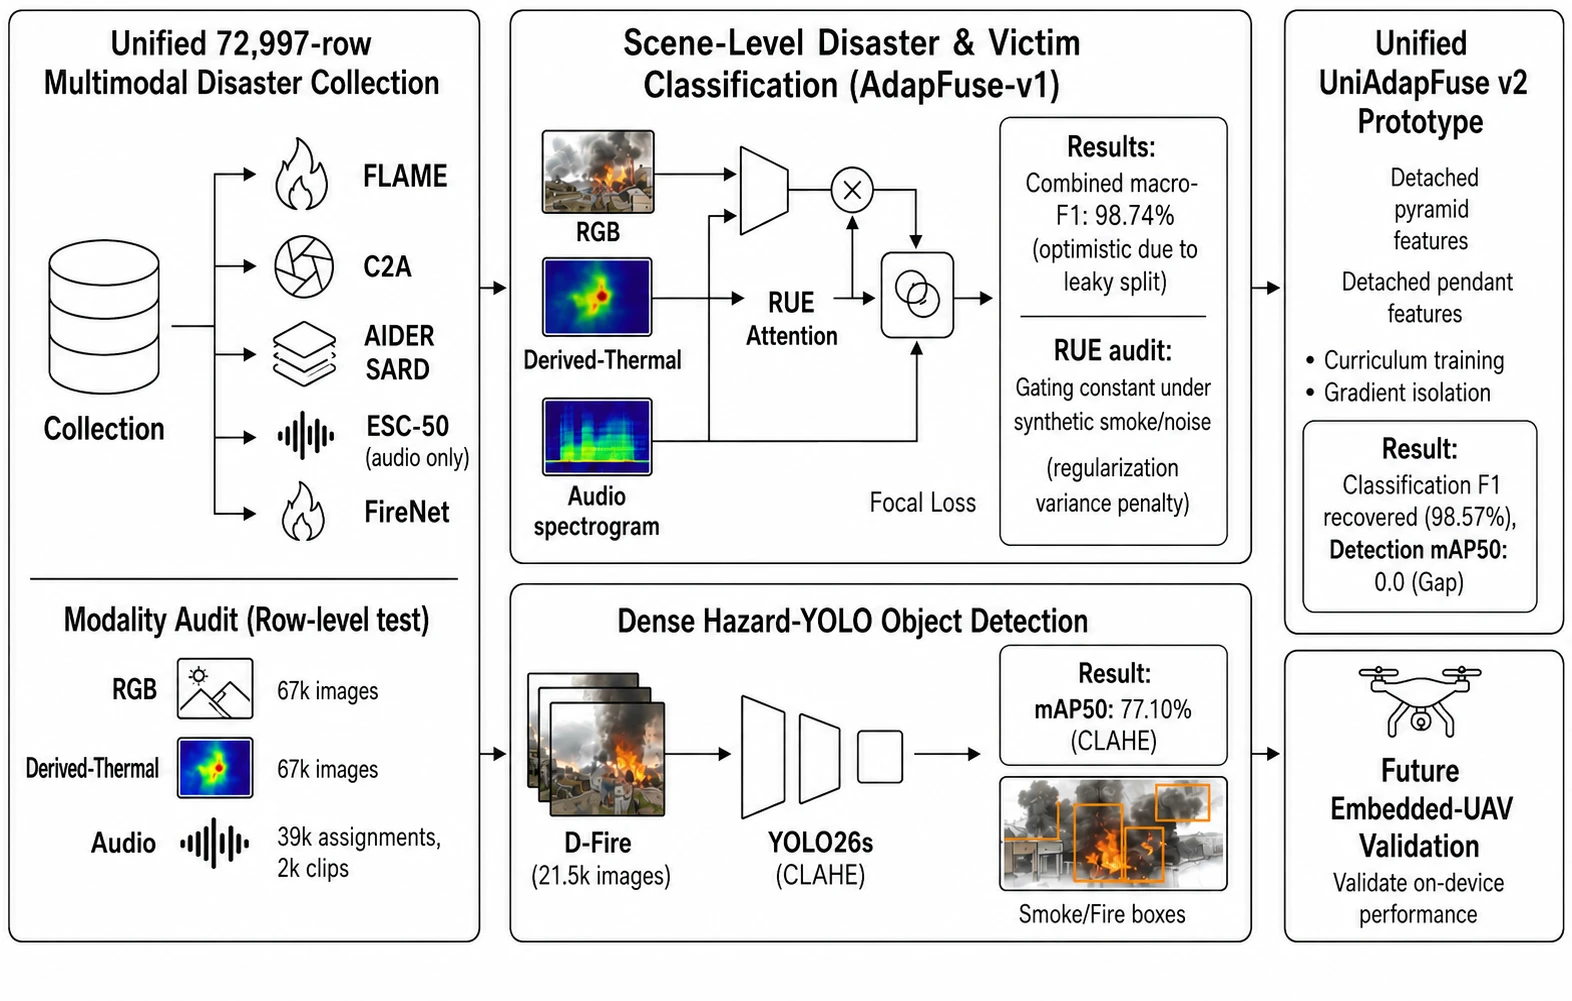
\includegraphics[width=0.8\textwidth]{1.png}
    \caption[Project overview]{Project overview. The 72{,}997-row multimodal collection supports scene-level disaster and victim-presence classification; the separate 21{,}527-image D-Fire benchmark supports smoke/fire detection. Solid boxes: measured results; dashed boxes: unvalidated or future work. The ``67k'' counts in the modality panel are outdated (correct: 70{,}997 RGB and 70{,}997 pseudo-thermal; Section~\ref{sec:dataset_sources}).}
    \label{fig:system_architecture}
\end{figure*}

\subsubsection{Phase 1: Dataset Assembly}

A unified 72{,}997-sample dataset was assembled from six public sources covering wildfire, structural collapse, crowd, and victim-presence scenarios:

\begin{itemize}
    \item \textbf{FLAME}~\cite{shamsoshoara2021aerial}: 47{,}992 UAV wildfire RGB frames, the largest source at 65.7\% of the dataset. In our metadata, its thermal entries are RGB-derived pseudo-thermal maps rather than sensor IR.
    \item \textbf{C2A}: 10{,}215 collapse and crowd aerial samples.
    \item \textbf{AIDER}~\cite{kyrkou2019aider}: 6{,}433 multi-class aerial disaster images (wildfire, flood, collapse, traffic).
    \item \textbf{SARD}: 5{,}755 search-and-rescue person-detection frames.
    \item \textbf{ESC-50}~\cite{piczak2015esc}: 2{,}000 environmental sound clips matched to visual samples by disaster label only, not by synchronized capture. A single clip is paired with many images from unrelated scenes, so the audio carries no information about the specific event in each image.
    \item \textbf{FireNet}: 602 fire and non-fire RGB frames.
\end{itemize}

For every RGB source in our metadata, pseudo-thermal maps were generated from the RGB frame; the metadata contains no sensor-IR path. ESC-50 clips were assigned to visual rows by label rather than synchronized capture: 39{,}003 rows reference only 2{,}000 unique audio files. A missing-modality flag tracks unavailable inputs, and training applies 20\% random single-modality dropout. The dataset was split by disaster-label stratification ($n_\text{train}=51{,}097$, $n_\text{val}=10{,}949$, $n_\text{test}=10{,}951$; total 72{,}997 rows). This split is not source-, flight-, or sequence-grouped, so its test metrics are within-collection rather than cross-flight estimates. A capture-group-aware split was therefore rebuilt (50{,}845 / 11{,}055 / 11{,}097 rows across 9{,}267 / 2{,}003 / 2{,}002 disjoint capture groups) and AdapFuse-v1 retrained on it: combined macro-F1 falls from 98.74\% to 89.14\%. That retraining was run without class balancing and with batch size 2, so the drop does not isolate the leakage effect (Section~\ref{sec:grouped_split}).

\textbf{Class balancing:} The raw training split is heavily imbalanced: fire/smoke (46.5\%), clean (41.0\%), collapse/flood (8.5\%), other (4.0\%). Due to a single-GPU resource constraint (NVIDIA RTX 5090, 32\,GB VRAM), a two-stage oversampling procedure was applied to generate a \textit{Stratified Balanced Training} configuration. Stage 1 oversamples each disaster class to the majority-class count via replacement sampling, marking synthetic duplicates with a synthetic-row indicator for stronger augmentation. Stage 2 oversamples the victim-positive class to achieve 50/50 victim balance while preserving disaster balance. The resulting full-balanced split (98{,}556 samples) is then halved with source-stratified sampling, which keeps all six dataset sources represented, yielding the final training split of 49{,}276 samples (exactly 12{,}319 per disaster class; 48.1\% synthetic rows). An equivalent procedure produces the validation split (10{,}516 stratified balanced samples). The held-out test set (10{,}951 samples) is \emph{never} resampled and retains the natural class distribution of the collection.

\subsubsection{Phase 2: Architecture Design}

Six core fusion designs along with architectural variants were implemented and compared on the same data split, balanced training subset and loss (learning-rate schedules differed between some runs; Table~\ref{tab:training}):

\textbf{Unimodal baselines:} Design A1 (RGB-only MobileNetV3-Small), A2 (Pseudo-thermal-only ResNet-18), and A3 (Audio-only 2D-CNN on mel-spectrograms) established per-modality performance bounds.

\textbf{Early Fusion (Design B):} A five-channel ResNet-18 receiving concatenated RGB, pseudo-thermal, and mel-spectrogram projections in the spatial domain.

\textbf{Late Fusion (Design C):} Three independent backbones producing softmax predictions fused by a learned linear combiner.

\textbf{Intermediate Fixed Fusion (Design D):} Backbone features projected to a shared 192-dim space and concatenated before a shared classification head, with no modality weighting.

\textbf{AdapFuse-v1 (Design E), proposed:} Three backbones (MobileNetV3-Small for RGB, ResNet-18 for thermal, 2D-CNN for audio) plus:
\begin{itemize}
    \item \textit{Reliability and Uncertainty Estimator (RUE):} An MLP reading 16-dim quality tokens and feature statistics per modality, producing scalar gates $r_i \in [0,1]$. In the reported training runs these gates are learned through task loss and a cross-modality variance regularizer, not explicit degradation labels.
    \item \textit{Cross-modal attention:} 4-head attention over reliability-weighted projected tokens stacked across all three modalities.
    \item \textit{NuisanceAwareHead:} The model defines disaster, victim-presence, and five-category nuisance logits. The current trainer supplies no nuisance ground truth, so only the disaster and victim branches are supervised in the reported checkpoints; nuisance-aware learning remains an architectural provision rather than an evaluated contribution.
\end{itemize}

\textbf{AdapFuse-v2 (Design F), knowledge-distilled student:} AdapFuse-v1 architecture with projection dimension reduced to 96 (half of the teacher's 192), trained with logit distillation (temperature $T=4.0$) and intermediate feature distillation ($\lambda=0.5$) from the Design E teacher.

\subsubsection{Phase 3: Training and Evaluation}

All twenty-six multimodal classification models (spanning core fusion designs, visual/acoustic backbone variants, architectural augmentations, two-sensor subsets, unified multi-task architectures, and isolated component ablations) were trained with AdamW (lr = $10^{-3}$, weight decay $10^{-4}$), cosine learning-rate decay with 5-epoch linear warmup, batch size 16 (reduced to 8 for EfficientNet-B0 backbone experiments due to larger feature dimensions), up to 50 epochs with early stopping (patience = 15), and automatic mixed precision (AMP). UniAdapFuse v2 departs from this recipe (Section~\ref{sec:uniadaptfuse}), and the logged learning-rate schedule is not identical across runs (Table~\ref{tab:training}). All row-level models use the Stratified Balanced Training Configuration (49{,}276 samples, exact 25\% per class); the grouped-split retraining (Section~\ref{sec:grouped_split}) is a separate run without class balancing. The implemented objective supports optional nuisance and degradation supervision, but our trainer passes both targets as None. The active base objective is therefore focal task loss plus reliability variance regularization:

\begin{equation}
    \mathcal{L} = w_d\,\text{FL}_{\text{disaster}} + w_v\,\text{FL}_{\text{victim}} + \lambda_r\,[-\operatorname{Var}(\mathbf{r})]
\end{equation}

The configuration files set corruption\_prob=0.3, but the base data-loader construction does not provide a corruption\_type; the explicit smoke, blur, low-light, drift, and audio-noise transforms are therefore not activated in the reported base training run. They are invoked only in the separate synthetic stress-test scripts. Evaluation on the held-out row-level split ($n=10{,}951$) uses macro-F1 for disaster and victim-presence classification. Knowledge distillation for Design F adds logit and feature losses on top of the task losses.

\subsection{Scopes and Challenges}

\textbf{In Scope:}
\begin{itemize}
    \item Multi-disaster classification (wildfire, structural collapse or flood, other hazards such as traffic incidents) and victim presence classification from UAV-sourced RGB imagery, RGB-derived pseudo-thermal maps, and label-matched acoustic clips~\cite{erdelj2017help}.
    \item Systematic comparison of six fusion architectures from unimodal baselines to adaptive attention-based fusion.
    \item Single-component comparison runs for the one-step GRU, cross-modal attention, learned quality features, auxiliary nuisance branch, and RUE gating.
    \item Investigation of multi-task negative transfer via phased curriculum training and stop-gradient feature isolation.
    \item Knowledge distillation for edge-deployment model compression~\cite{hinton2015distilling}.
    \item An implemented nuisance-class branch, with supervised nuisance learning left for future labeled experiments.
    \item Environmental corruption stress testing across five severity levels, and missing-modality checks through two-sensor subsets and simulated sensor dropout.
\end{itemize}

\textbf{Out of Scope:} Physical in-flight edge deployment on an active UAV airframe with live payload actuation, long-term post-disaster reconstruction planning, and autonomous UAV aerodynamic path planning. These are identified as priority future directions in Chapter~6.

\textbf{Key Challenges Encountered:}
The audio modality presented the most significant practical challenge: ESC-50 clips are general environmental sounds paired by label rather than captured synchronously with the same disaster scene. The pairing also leaks the label: every fire-labelled row with audio receives one of the 40 ESC-50 ``crackling fire'' clips, every clean row receives a clip from the other 49 classes, and no collapse/flood or other-hazard row has audio. The audio-only baseline (Design A3) therefore scores only 38.2\% disaster macro-F1 overall, although its accuracy is consistent with near-perfect fire/clean prediction on the rows that have audio. The row-level AdapFuse-v1 checkpoint gives audio a near-zero gate, whereas the grouped retraining keeps it fully open, so whether a fused model uses this shortcut depends on the run. Every populated thermal path points to an RGB-derived pseudo-thermal map, including FLAME and C2A; no sensor-IR frames are present in our metadata. The high prevalence of FLAME creates a visually dominant source, and the row-level split proved to be a substantial explanation for the narrow, near-ceiling performance range: retraining under capture-group-aware splitting scores 9.60 percentage points lower in combined macro-F1, although that retraining also differed in class balancing and batch size. Decomposing those grouped predictions by source exposes a second problem: source identity and label are confounded in the assembled corpus. Victim presence is fully determined by the source dataset in the grouped test set, and several sources contain a single disaster class, so aggregate scores cannot distinguish hazard or person recognition from dataset recognition.


%=====================================================================
\section{Literature Review}
%=====================================================================

%*******************************************************************
% Chapter 2: Related Work
% UniAdapFuse: Reliability-Aware Multimodal Fusion for
% UAV Disaster Perception
%*******************************************************************

\subsection{Related Work}

This chapter surveys prior research across the foundational pillars of our framework: (1) single-modality aerial sensing and physical failure modes; (2) multimodal fusion architectures and 2024--2026 contemporary SOTA paradigms; (3) real-time aerial object detection and vision transformers; (4) multi-task negative transfer in unified perception; and (5) edge-deployment compression on UAV embedded hardware. For each domain, we analyze existing methodologies, identify critical failure modes, and establish the technical rationale for the architectural innovations in \textbf{UniAdapFuse}.

\subsubsection{Single-Modality Aerial Sensing and Environmental Failure Modes}

The three primary modalities used in aerial UAV disaster response (RGB visual cameras, thermal infrared sensors, and acoustic microphones) capture fundamentally distinct physical phenomena, exhibiting complementary strengths and misaligned failure modes.

\textbf{RGB Visual Sensing.}
Visible-light cameras provide high spatial resolution (typically $1920\times1080$ to $4\text{K}$) and rich chromatic signatures essential for distinguishing flame color palettes, smoke plume textures, and human survivor clothing~\cite{celik2009fire, toreyin2006computer}. Deep convolutional neural networks (CNNs) have achieved high image-level fire detection and localization accuracy in video surveillance settings~\cite{muhammad2019efficient}. However, RGB systems are physically vulnerable: dense wildfire smoke obscures the scene, nighttime flight removes chromatic information, and solar glare saturates camera sensors. These failure modes are limits of optical sensing itself, so a larger RGB model cannot remove them.

\textbf{Thermal Infrared Imaging.}
Thermal infrared sensors detect long-wave infrared radiation (LWIR, 7.5--14 $\mu$m) emitted as blackbody radiation proportional to object temperature. Thermal imaging operates independently of ambient illumination, penetrating darkness, light smoke, and foliage haze to detect active combustion zones and $37^\circ\text{C}$ living human body heat~\cite{toulouse2017computer}. However, aerial thermal sensing carries severe operational limitations: typical UAV thermal sensors have low spatial resolution ($320\times240$ px), preventing distant survivor detection from high altitudes ($>50$ m). Furthermore, solar heating can raise asphalt, dry soil, and metal roofs well above body temperature in daytime flight, which can trigger false-positive detections. In fusion models with fixed modality weights, these solar thermal artifacts can mislead the network and produce excessive false alarms.

\textbf{Acoustic Sensing and UAV Rotor Noise.}
Acoustic sensors capture pressure waves that propagate around visual occlusions and can carry signatures of burning, structural collapse, and human calls for help. However, the rotors of the UAV itself produce strong ego-noise that lowers the signal-to-noise ratio (SNR) of on-board recordings~\cite{gupta2025droneaudioset}. This motivates gating mechanisms that down-weight acoustic tokens when noise dominates.

\subsubsection{Real-Time Aerial Object Detection and Vision Transformers}

Autonomous UAV disaster response requires \textbf{dense 2D bounding box localization} $(\text{xmin}, \text{ymin}, \text{xmax}, \text{ymax})$ to direct tactical fire suppression and rescue operations.

\textbf{Anchor-Free Convolutional Detectors (YOLO Series).}
The You Only Look Once (YOLO) family represents the standard for real-time edge detection. Recent versions including YOLOv8, YOLOv10~\cite{wang2024yolov10}, YOLO11~\cite{ultralytics2024yolo11}, and YOLO26~\cite{sapkota2025yolo26} use anchor-free heads; YOLO11 and YOLO26 build on C3k2 cross-stage blocks, and YOLOv10 and YOLO26 support end-to-end inference without Non-Maximum Suppression (NMS). On the D-Fire smoke and fire benchmark~\cite{dfire2022}, the nano-scale detectors trained in this work reach 67.75\% to 72.58\% $\text{mAP}_{50}$. Standard YOLO architectures learn all their filters from data and use no physical domain priors. UniAdapFuse therefore includes a \textbf{Hazard Prior Gate (HPG)}, which computes red-excess chromaticity, achromaticity and edge cues from the input frame and applies a bounded residual correction before the detector stem. In our runs it does not help: it lowers $\mathrm{mAP}_{50}$ by 0.94 points and trains about $1.9\times$ slower than the baseline YOLO26n (8.65 versus 4.45 hours for the same 40 epochs).

\textbf{Real-Time Detection Transformers (RT-DETR).}
To eliminate handcrafted NMS post-processing, RT-DETR~\cite{zhao2024rtdetr} introduces deformable multi-scale cross-attention with bipartite Hungarian matching. The RT-DETRv2-R18 variant reaches $73.8\%\, \text{mAP}_{50}$ on D-Fire in this work (Table~\ref{tab:dfire_results}), but its attention modules are more demanding in memory than nano-scale YOLO models, which matters on small UAV platforms; we did not measure its power draw.

\subsubsection{Public Benchmarks for Aerial Disaster Classification and Fire Detection}
\label{sec:public_benchmarks_related}

Three public datasets used in this thesis have published protocols against which single-modality results can be compared.

\textbf{AIDER.} Kyrkou and Theocharides introduced the AIDER aerial emergency dataset with a lightweight classifier~\cite{kyrkou2019aider} and later EmergencyNet, which uses atrous convolutional feature fusion to classify drone imagery at low cost~\cite{kyrkou2020emergencynet}. Lee et al.\ re-trained six lightweight CNNs from scratch on the 6{,}433-image AIDER subset with the 4:1:2 train/validation/test protocol (2{,}473 test images, class-imbalanced towards the normal class) and proposed WATT-EffNet, a wider, attention-augmented EfficientNet under 1\,M parameters~\cite{lee2023wattefnet}. Under that protocol they report F1 scores of 80.0\% for EfficientNet, 81.0\% for MobileNetV2, 83.1\% for EmergencyNet and 88.5\% for WATT-EffNet. Later ultra-lightweight networks, TinyEmergencyNet~\cite{mogaka2024tinyemergencynet}, TakuNet~\cite{rossi2025takunet} and GlimmerNet~\cite{nedeljkovic2025glimmernet}, report 89.5--94.2\% weighted F1 with fewer than 0.1\,M parameters under the earlier Kyrkou split.

\textbf{FLAME.} Shamsoshoara et al.\ released FLAME with a fixed fire/no-fire classification split in which the 39{,}375 training frames come from one drone and camera (Matrice 200, Zenmuse X4S) and the 8{,}617 test frames from another (Phantom 3). Their Xception classifier reaches 76.23\% test accuracy~\cite{shamsoshoara2021aerial}. Later work on the same test frames raised this to 85.12\% with an EfficientNet-B5/DenseNet-201 ensemble~\cite{ghali2022uavwildfire}, 87.32\% with FireXplainNet~\cite{khan2024firexplainnet} and 88.05\% with an ensemble of attention-augmented MobileNetV2 models~\cite{deng2025lightweight}. Because the camera changes between training and test, this protocol measures cross-camera generalisation, which a random frame-level split does not.

\textbf{D-Fire.} De Ven\^{a}ncio et al.\ built D-Fire (21{,}527 images with smoke and fire boxes) and showed that filter pruning can cut YOLOv4's computational cost by up to 83.60\% for low-power fire detection~\cite{dfire2022}; the pruned detector is reported to keep the baseline's 73.98\% mAP. Published detectors report 79.46\% $\mathrm{mAP}_{50}$ for YOLOv5l~\cite{venancio2023hybrid}, 80.40\% for YOLOv7x~\cite{goncalves2024yolo} and 79.04\% for YOLOv8m averaged over three seeds~\cite{ruangsang2026crossdataset}, each on the test set used in its own study. We train and test our detectors on our own 70/20/10 re-split (15{,}069 train, 4{,}305 val, 2{,}153 test), so these published figures are reference points rather than results on our test images. Ruangsang and Pramkeaw also found near-duplicates of training images in 46.0\% of the original official test images~\cite{ruangsang2026crossdataset}; our re-split avoids this contamination.

These works are single-modality and evaluate each dataset under its own protocol. Section~\ref{sec:public_benchmark_results} trains our models under the AIDER and FLAME protocols, and Section~\ref{sec:object_detection} places our D-Fire detectors beside the published detectors, so that both can be compared with these results.

\subsubsection{Contemporary 2024--2026 Multimodal SOTA Literature}

Multimodal fusion for aerial robotics has advanced rapidly from static concatenation to dynamic gating:

\begin{itemize}
    \item \textbf{UAV RGB-Thermal Fusion Dataset and Model (Zhang et al., 2025)~\cite{zhang2025rgbt}:} A UAV-collected multi-scenario RGB-thermal dataset paired with a fusion model for enhanced forest fire detection. While effective for paired optical-thermal imagery, it lacks acoustic integration, physical hazard priors, and nuisance false-alarm modeling.
    \item \textbf{Multi-Modal Training Dynamics (Wang et al., 2020)~\cite{wang2020makes}:} Wang et al.~\cite{wang2020makes} investigated the challenges of training multi-modal classification networks, including modality-specific overfitting and generalization. However, their analysis does not address UAV-specific rotor noise, thermal sensor drift, or explicit physical nuisance modeling.
    \item \textbf{DeepFire (Khan et al., 2022)~\cite{khan2022deepfire}:} DeepFire~\cite{khan2022deepfire} provides a dataset and deep transfer-learning benchmark for forest-fire detection. It is RGB-only and therefore offers no mechanism to down-weight a blinded camera during heavy smoke.
    \item \textbf{DroneAudioset (Gupta et al., 2025)~\cite{gupta2025droneaudioset}:} A 23.5-hour synchronized UAV SAR acoustic dataset with measured rotor-noise profiles, providing the empirical foundation for acoustic search-and-rescue and noise-resilient multimodal fusion.
\end{itemize}

\subsubsection{Multi-Task Learning and Negative Transfer in Unified Vision}

Simultaneous prediction of global scene semantics (disaster categorization, sensor trust) and dense spatial objects (bounding box regression) within a single shared backbone is notoriously vulnerable to \textbf{multi-task negative transfer}~\cite{yu2020gradient}. When dense regression losses (CIoU and objectness) are backpropagated concurrently with classification losses, high-magnitude localization gradients disrupt the shared feature representations, which can cause classification accuracy to drop. Our naive UniAdapFuse v1 run reached only 53.7\% disaster accuracy, against 99.4\% for the classification-only AdapFuse-v1, although its training log also shows many batches skipped for non-finite losses, so negative transfer is not the only possible explanation (Section~\ref{sec:uniadaptfuse}).

Prior multi-task works attempt to mitigate this through gradient surgery (e.g., PCGrad) or loss weighting. In this work, a revised recipe combining a 15-epoch classification warmup, stop-gradient isolation (.detach()) on multi-scale feature pyramids, and knowledge distillation from AdapFuse-v1 recovers scene classification to 98.57\% Combined F1; because these changes were made together, their individual contributions are not identified. The recorded detection $\mathrm{mAP}_{50}$ for that joint checkpoint is 0.0, so the result demonstrates classification recovery but not successful joint localization.

\subsubsection{Edge Deployment and Knowledge Distillation}

Embedded UAV compute platforms (typically constrained to strict 10--15W power envelopes) impose severe memory and latency constraints. While structured pruning~\cite{zhu2017prune} and INT8 quantization~\cite{jacob2018quantization} compress individual backbones, compressing multi-branch multimodal networks requires preserving cross-modal alignment. Knowledge distillation (KD)~\cite{hinton2015distilling} transfers rich relational features from a high-capacity teacher to a compact student. In our framework, AdapFuse-v2 leverages feature and logit KD to halve the shared projection width (192 $\to$ 96). Because the two dominant visual backbones (ResNet-18, MobileNetV3-Small) are untouched by this change, the measured total parameter reduction is modest, 12.94M $\to$ 12.30M (4.9\%), rather than a proportional halving; the teacher AdapFuse-v1 measures 14.32 ms per frame (69.9 FPS) on the evaluation workstation GPU, and dedicated edge-hardware profiling of the distilled student is left to future work (see Chapter~6).

\subsubsection{Research Gaps and Synthesis}

Table~\ref{tab:sota_gap_map} synthesizes the identified literature gaps and maps them to our architectural solutions.

\begin{table*}[!t]
\centering
\caption[Literature gaps and UniAdapFuse responses]{Literature gaps and UniAdapFuse architectural responses}
\label{tab:sota_gap_map}
\resizebox{\textwidth}{!}{%
\begin{tabular}{p{4.2cm} p{5.5cm} p{5.5cm}}
\toprule
\textbf{Literature Gap} & \textbf{UniAdapFuse Architectural Response} & \textbf{Observed Empirical Outcome} \\
\midrule
No physical priors in data-driven detectors & \textbf{Hazard Prior Gate (HPG):} Red-excess, achromaticity and edge cues drive a bounded residual correction of the input frame & Not supported: $70.53\%\, \text{mAP}_{50}$ in 8.65\,h vs.\ $71.47\%$ in 4.45\,h for YOLO26n ($-0.94$ pp, $1.9\times$ slower) \\
\addlinespace
Multi-task negative transfer in joint perception & \textbf{Curriculum Warmup \& Stop-Gradient Isolation:} Detaches pyramid features before detection neck (applied together with distillation from AdapFuse-v1) & Disaster accuracy recovered from $53.71\% \to 99.26\%$, effect of each change not isolated; joint detection $\mathrm{mAP}_{50}=0.0$ \\
\addlinespace
Static fusion weights under camera failure & \textbf{Reliability \& Uncertainty Estimator (RUE):} Learned scalar gates $r_i \in [0,1]$ & Smoke-overlay F1 is 89.7\% at severity 5, but saved gates remain nearly constant (no dynamic reweighting shown), no matched static baseline is logged, and fused F1 (98.74\%) does not exceed RGB-only (98.85\%) \\
\addlinespace
False alarms on hazard look-alikes & \textbf{5-Class NuisanceAwareHead:} Defines logits for clean signal, solar heating, false fire, audio alarm, occlusion & Branch is unsupervised in our run; 0.73\% is a row-level classifier FPR, not a nuisance-head effect \\
\addlinespace
Edge compute bottleneck on embedded UAVs & \textbf{Knowledge Distillation (AdapFuse-v2):} Halves projection width via logit \& feature KD & 12.30M params (4.9\% smaller) with $<0.2$ pp F1 loss; teacher runs at 14.32 ms (69.9 FPS) on the workstation, edge-GPU profiling of the student left to future work \\
\bottomrule
\end{tabular}%
}
\end{table*}


%=====================================================================
\section{Requirements, Impacts and Constraints}
%=====================================================================

%*******************************************************************
% Chapter 3: Requirements, Impacts and Constraints
%*******************************************************************

\subsection{Final Specifications and Requirements}

This section establishes the concrete hardware, software, and data requirements that the UniAdapFuse system must satisfy. These specifications are derived from operational disaster-response constraints rather than idealised laboratory conditions, ensuring that design decisions remain grounded in real-world deployability. They are target specifications set at the planning stage, not results; Table~\ref{tab:req_trace} in the Conclusion reports which of them our system meets.

\subsubsection{Technical Requirements}
\label{sec:tech_requirements}

\textbf{Sensor Hardware Requirements:}
\begin{itemize}
    \item \textbf{RGB Camera:} Minimum 1920$\times$1080 resolution at 30 FPS; field of view $\geq 80^{\circ}$; electronic image stabilisation to mitigate rotor vibration blur
    \item \textbf{Thermal Infrared Camera:} Minimum 320$\times$240 resolution at 10 FPS; NETD $\leq$50\,mK; spectral band 7.5--14\,$\mu$m (LWIR); operating range $-20$\,\textdegree{}C to $+550$\,\textdegree{}C
    \item \textbf{Acoustic Module:} 2-element microphone array (minimum), sampling rate 16 kHz; SNR $\geq$60 dB; vibration isolation mount to suppress rotor-induced mechanical noise
    \item \textbf{Edge Compute Payload (Target Specification):} Low-power embedded edge GPU (minimum 8 GB RAM); TDP $\leq$15 W; operating temperature $-25$\,\textdegree C to $+80$\,\textdegree C; mass $\leq 280$\,g
\end{itemize}

\textbf{Software and Algorithm Requirements:}
\begin{itemize}
    \item End-to-end inference latency $\leq$500 ms from sensor capture to classification output at 10 FPS
    \item Detection accuracy $\geq$95\% for wildfire scenes (RGB+thermal fusion); $\geq$90\% for USAR victim detection across all lighting conditions
    \item False positive rate $\leq$8\% under operational conditions including solar heating, dust, glare, and rotor noise
    \item Graceful degradation: system must maintain $\geq$85\% accuracy when any single modality is unavailable
    \item INT8 quantisation-aware inference for all modality encoders
    \item Timestamp alignment tolerance $\leq$50 ms across all sensor streams
\end{itemize}

\textbf{Data Requirements:}
\begin{itemize}
    \item Curated multimodal dataset: $\geq$6,000 synchronised (RGB, thermal, audio) sequences covering wildfire and USAR scenarios
    \item Balanced class ratio with minimum 40\% negative samples to avoid overfitting
    \item Training/validation/test split: 70\%/15\%/15\%, stratified by scenario type and environmental condition
    \item Augmentation pipeline supporting synthetic degradation: smoke occlusion, sensor dropout, rotor noise injection
\end{itemize}

\subsubsection{Functional Requirements}

The system shall perform three primary functions that together constitute the disaster detection pipeline.

\begin{enumerate}
    \item \textbf{Disaster Detection:} Binary classification (disaster present / absent) with per-class confidence scores for fire, smoke, and structural collapse
    \item \textbf{Victim-Presence Classification:} Classification of whether a person/victim is present or absent in the input sample, with individual confidence scores
    \item \textbf{Modality Reliability Estimation:} Online estimation of per-modality reliability scores $r_i \in [0,1]$ used as inputs to the adaptive attention gating network
\end{enumerate}

\subsection{Societal Impact}

The proposed framework aims to improve disaster response by enabling faster and more reliable detection from UAV platforms. A wildfire detected early can be engaged while it is still small~\cite{merino2012unmanned}, and in USAR operations the chance of rescuing survivors falls with elapsed time~\cite{erdelj2017help}. Sub-500 ms onboard inference is set as a target so that detection does not become the bottleneck in these time windows.

Reliable automated detection could also reduce the burden on emergency dispatch infrastructure. False alarms from automated fire detectors lead to unnecessary dispatches, and each one consumes personnel time, fuel, and response capacity elsewhere. Reducing false positives to $\leq$8\% in the field (our target) would save resources and improve operator trust; the 0.73\% false-positive rate reported in Chapter~5 is a row-level test statistic, not an operational field rate.

The framework also benefits remote and underserved communities where ground-based sensor networks are economically infeasible and satellite revisit cycles (5--16 days) are insufficient for active disaster monitoring.

\subsection{Environmental Impact}

This section considers both the positive environmental effects of earlier disaster detection and the energy footprint of the proposed system itself.

\textbf{Positive environmental effects:} Earlier wildfire detection limits uncontrolled burn area and associated carbon emissions. A fire detected 30 minutes earlier than conventional methods can be engaged while it is still small, limiting the area burned before suppression begins, with commensurate reductions in CO$_2$, particulate matter, and volatile organic compound emissions.

\textbf{Energy considerations:} The planned onboard edge-compute module (target $\leq$10--15 W) would avoid the continuous high-bandwidth uplink that cloud inference requires. INT8 quantised inference is expected to lower compute energy per frame relative to FP32, but quantisation was not implemented in this work, so neither the energy saving nor its effect on flight time was measured.

\textbf{Manufacturing impact:} The sensor payload (RGB camera, thermal module, microphone array, edge compute module) is estimated to add 600--900 g to the UAV payload. This manufacturing footprint is offset across repeated operational deployments over the system lifetime.

\subsection{Ethical Issues}

Deploying UAV-based detection systems in populated and disaster-affected areas raises several ethical considerations that must be addressed in system design and operational policy.

\textbf{Aerial privacy:} UAV-mounted cameras operating over populated areas capture incidental imagery of individuals not involved in disaster scenarios. Mitigations include: strict data retention limits (raw sensor streams purged within 72 hours); on-device inference ensuring raw imagery is not transmitted externally; and operational policies restricting UAV flights to declared disaster zones with appropriate authority clearance.

\textbf{Algorithmic fairness:} Victim detection models trained predominantly on Western disaster datasets may exhibit performance disparities across demographic groups. Systematic evaluation across skin tones, body sizes, and cultural clothing is required before operational deployment.

\textbf{Automation of life-critical decisions:} Detection outputs must support human emergency managers rather than trigger autonomous action. The system is intended to provide calibrated confidence scores to enable informed human oversight; calibration is measured only on the row-level test split (ECE 0.0337) and has not been validated in the field.

\textbf{Dual-use risk:} Surveillance technology developed for disaster detection could be repurposed for unauthorised monitoring. Deployment policies, audit logging, and hardware tamper-evidence mechanisms are required in institutional deployments.

\subsection{Standards}

A deployable version of the system would need to address the following standards. The research prototype has not been assessed for conformance with any of them; they are listed to scope future engineering work.

\begin{itemize}
    \item \textbf{IEEE 1512:} Standard for Common Incident Management Message Sets for Emergency Management Centers; governs detection output data formats
    \item \textbf{ISO 9001:2015:} Quality management requirements applied to dataset curation, annotation, and model evaluation
    \item \textbf{STANAG 4586 / NATO UAVNET:} UAV interoperability standards for data link protocols and payload command interfaces
    \item \textbf{IEC 62443:} Industrial cybersecurity standard applied to UAV-to-ground-station communication to prevent adversarial interference
    \item \textbf{RTCA DO-178C:} Software considerations for airborne systems; applied to safety-critical inference pipeline components
\end{itemize}

\subsection{Project Management Plan}

This section outlines the planned development phases and resource requirements for the UniAdapFuse project, along with a risk register identifying key threats to successful completion. Table~\ref{tab:project_schedule} lists the five development phases and their corresponding deliverables.

\begin{table*}[!t]
\centering
\caption{Project milestones and deliverables}
\label{tab:project_schedule}
\begin{tabular}{@{}lp{8cm}@{}}
\toprule
\textbf{Phase} & \textbf{Deliverable} \\
\midrule
Phase 1: Dataset Curation      & Curated multimodal dataset ($\geq$6,000 sequences), annotation pipeline, quality audit \\
Phase 2: Architecture Design   & Modality encoder implementations, attention fusion module, training scripts \\
Phase 3: Training \& Ablation  & Trained baseline and ablation models, accuracy and latency benchmarks \\
Phase 4: Edge Optimisation     & INT8 quantised models, TensorRT deployment pipeline, projected edge hardware latency profiles \\
Phase 5: Evaluation \& Writing & Full evaluation results, thesis chapters, submitted manuscript \\
\bottomrule
\end{tabular}
\end{table*}

\textbf{Resource allocation:} Primary compute resources comprise one NVIDIA RTX 5090 workstation (32\,GB VRAM) for model training and simulation. Physical deployment onto dedicated embedded edge hardware is reserved for future operational benchmarking. Dataset storage requires approximately 2 TB. No field data collection hardware is required as the dataset leverages publicly available sources augmented synthetically.

\subsection{Risk Management}

Risk management is essential for a project that combines hardware integration, novel deep learning, and operational deployment constraints. Table~\ref{tab:risk_register} summarises key risks, their estimated likelihood and impact, and the planned mitigations.

\begin{table*}[!t]
\centering
\caption{Project risk register}
\label{tab:risk_register}
\begin{tabular}{@{}p{4cm}ccp{4.5cm}@{}}
\toprule
\textbf{Risk} & \textbf{Likelihood} & \textbf{Impact} & \textbf{Mitigation} \\
\midrule
Dataset class imbalance & High & High & Focal Loss; oversampling; synthetic augmentation \\
Latency target not met post-quantisation & Medium & High & QAT from training start; structured pruning fallback \\
Rotor noise rendering audio unusable & Medium & Medium & Spectral subtraction; treat audio as optional; ablation without audio. \textit{Risk materialised}: no real UAV audio was available; the label-matched ESC-50 audio leaks the fire/clean label (Section~\ref{sec:unimodal_backbones}) \\
Domain shift between synthetic and real data & High & Medium & Domain randomisation; held-out real-world test set \\
Thermal false positives from solar heating & Medium & Medium & Time-of-day conditioning; joint RGB+thermal decision boundary \\
Compute hardware failure & Low & High & Cloud training backup; checkpoints every 5 epochs \\
\bottomrule
\end{tabular}
\end{table*}

\subsection{Economic Analysis}

The following illustrative cost analysis rests on the stated assumptions rather than on field data; it indicates that a UAV-based system could offer a favourable return on investment relative to fixed monitoring infrastructure.

\textbf{Development costs:} The saved training logs account for roughly 390 GPU-hours (about 280 for classification and 110 for detection); this is a lower bound because some resumed runs kept only part of their history. At assumed cloud-equivalent rates of \$0.30--\$0.90 per GPU-hour, this is about \$120--\$350 of compute, plus dataset storage (\$50/month).

\textbf{Deployment cost per UAV:} Sensor payload (thermal \$800--\$2,000; RGB camera \$300; microphone array \$50; edge compute module \$400) totals \$1,550--\$2,750. The medium-class UAV platform (\$8,000--\$15,000) is the dominant cost. Compared to fixed ground sensor networks (\$50,000--\$200,000 per installation), UAV-based deployment provides substantially better cost-per-covered-area for active disaster monitoring.

\textbf{Benefit estimation:} Assuming that 30\% of dispatches are avoidable false alarms in a region with 100 dispatch events per year, at \$5,000 saved per avoided dispatch, the system generates approximately \$150,000 in avoided costs annually, recovering deployment cost within the first operational year.


%=====================================================================
\section{Proposed Methodology}
%=====================================================================

%*******************************************************************
% Chapter 5: Proposed Methodology
%*******************************************************************

\subsection{Design Process Overview}

The proposed methodology follows four phases: (1) multimodal dataset curation from heterogeneous public sources, (2) design and comparison of six fusion architectures, (3) training with missing-modality simulation (synthetic corruptions are applied only in separate offline stress tests), and (4) evaluation on a held-out test set. Figure~\ref{fig:pipeline_overview} shows the end-to-end pipeline from raw sensor inputs to classification output.

\begin{figure*}[!t]
\centering
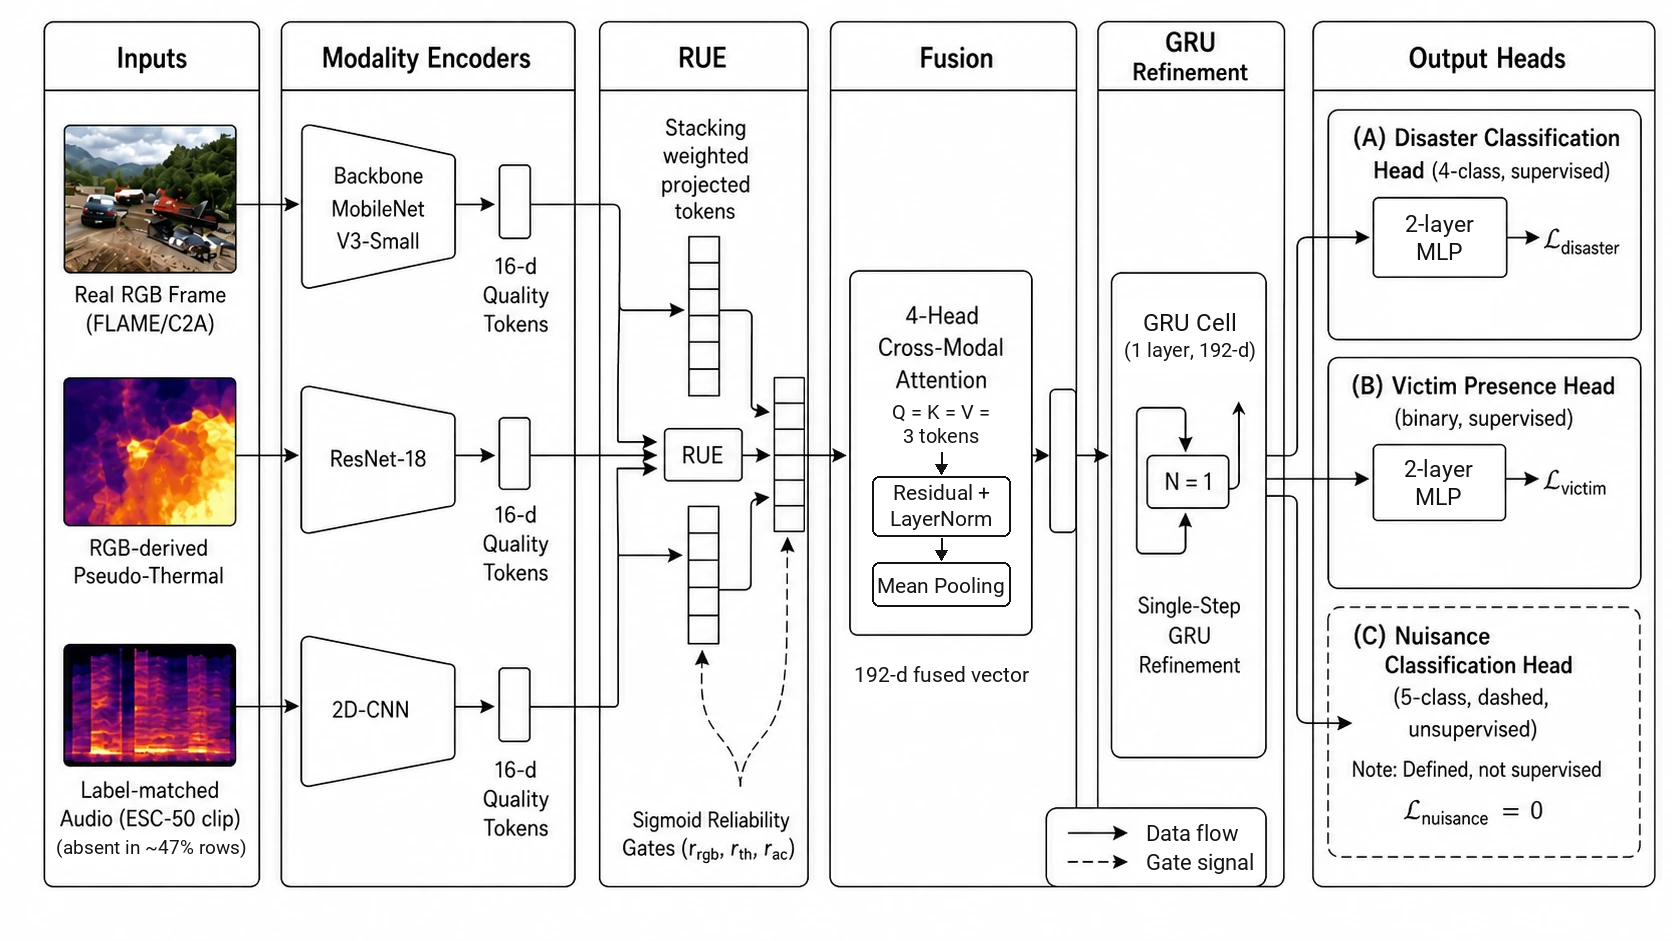
\includegraphics[width=0.8\textwidth]{4.1.png}
\caption[AdapFuse-v1 architecture]{AdapFuse-v1 architecture. \textbf{Inputs:} an RGB frame, its RGB-derived pseudo-thermal map, and a label-matched ESC-50 audio clip as a log-mel spectrogram (absent in about 47\% of rows). \textbf{Modality encoders:} MobileNetV3-Small, ResNet-18 and a small 2D-CNN; each gives a 192-d projected feature token and a 16-d quality token describing input quality. \textbf{RUE} (Reliability and Uncertainty Estimator): an MLP that reads the quality tokens and feature statistics and outputs one sigmoid reliability gate per modality, $r_{\mathrm{rgb}}, r_{\mathrm{th}}, r_{\mathrm{ac}} \in [0,1]$ (set to 0 when that input is missing); each token is multiplied by its gate. \textbf{Fusion:} 4-head attention across the three weighted tokens ($Q=K=V$), a residual connection with LayerNorm, then mean pooling to one 192-d vector. \textbf{GRU refinement:} one GRU cell run for a single step ($N=1$), so it refines the vector but keeps no memory across frames. \textbf{Output heads:} two-layer MLPs for disaster type (4 classes) and victim presence (2 classes), trained with $\mathcal{L}_{\mathrm{disaster}}$ and $\mathcal{L}_{\mathrm{victim}}$; the dashed nuisance head (5 classes) gets no labels, so $\mathcal{L}_{\mathrm{nuisance}}=0$. Solid arrows: data flow; dashed arrows: gate signals.}
\label{fig:pipeline_overview}
\end{figure*}

\subsection{Dataset Curation}

\subsubsection{Sources and Composition}
\label{sec:dataset_sources}

Because no single public dataset provides synchronized RGB, thermal, and audio for UAV disaster detection, the dataset was assembled from six public sources and unified under a structured metadata catalogue. Table~\ref{tab:dataset_sources} lists each source, the disaster scenario it covers, and its contribution.

\begin{table*}[!t]
\centering
\caption[Dataset sources and contribution]{Dataset sources and contribution to the unified metadata}
\label{tab:dataset_sources}
\resizebox{\textwidth}{!}{%
\begin{tabular}{@{}llccp{5cm}@{}}
\toprule
\textbf{Source} & \textbf{Scenario} & \textbf{Modalities} & \textbf{Samples} & \textbf{Notes} \\
\midrule
FLAME~\cite{shamsoshoara2021aerial}      & Wildfire                  & RGB + derived map & 47{,}992 & Aerial UAV RGB footage; pseudo-thermal paths are derived from RGB. Largest source. \\
C2A~\cite{nihal2024c2a}                  & Crowd / victim            & RGB            & 10{,}215 & Synthetic composites: human poses overlaid on UAV disaster scenes; every row victim-positive \\
AIDER~\cite{kyrkou2019aider}             & Multi-disaster (fire, flood, collapse, traffic, normal) & RGB & 6{,}433 & Benchmark for aerial disaster scene classification \\
SARD~\cite{sambolek2021sard}             & Victim (person visible)   & RGB            & 5{,}755  & Aerial person search dataset; victim\_label=1 per sample \\
ESC-50~\cite{piczak2015esc}             & Audio events              & Audio          & 2{,}000  & Audio-only rows; clips also reused across 39{,}003 assigned metadata rows; label-matched, not synchronized \\
FireNet~\cite{jadon2019firenet}          & Wildfire                  & RGB            & 602      & Video frames; additional fire/no-fire RGB samples \\
\midrule
\textbf{Total unique} & & & \textbf{72{,}997} & Raw: Train 51{,}097 / Val 10{,}949 / Test 10{,}951 \\
\textbf{Training (used)} & & & \textbf{49{,}276} & Stratified Balanced Subset: 12{,}319 per disaster class \\
\bottomrule
\end{tabular}%
}
\end{table*}

\textbf{Label schema:} Each sample carries two independent labels. The \textit{disaster label} takes values 0 (clean), 1 (fire/smoke), 2 (structural collapse or flood), or 3 (other hazard). The \textit{victim label} takes values 0 (no person visible) or 1 (person visible).

\textbf{Modality availability:} Not all sources supply all three inputs. Each row carries three Boolean presence flags (RGB, pseudo-thermal, and audio). Missing inputs are zero-filled and the corresponding flag is cleared. Recomputing the metadata shows 70{,}997 RGB paths and 70{,}997 pseudo-thermal paths, with every thermal path under the RGB-derived pseudo\_thermal tree and no sensor-IR path. Audio is available in 39{,}003 rows but draws from only 2{,}000 unique ESC-50 files, assigned by label rather than capture time. Audio exists only for clean (0) and fire/smoke (1) rows: all 20{,}433 fire/smoke rows with audio share the 40 clips of the ESC-50 ``crackling fire'' class, and all 18{,}570 clean rows with audio draw from the other 1{,}960 clips. The 2{,}000 ESC-50 rows themselves have no image and are the difference between the 72{,}997 rows and the 70{,}997 image paths. In the test set, 10{,}646 of 10{,}951 rows (97.2\%) have RGB and pseudo-thermal, while 5{,}781 (52.8\%) have an assigned audio clip. Nearly half of the test rows are therefore evaluated without any audio input, and every aggregate test score mixes rows with and without audio.

\textbf{Consequences of the data construction.} Two properties of our metadata limit what the multimodal experiments can show. First, the pseudo-thermal stream is computed from the RGB frame, not measured by independent LWIR hardware; RGB + pseudo-thermal fusion therefore combines two representations of one sensor, cannot reveal phenomena invisible to RGB (such as heat sources in darkness), and degrades together with RGB. Second, the ESC-50 audio is assigned by shared label rather than recorded with the frame, so the same clip is paired with many unrelated images and carries no scene-specific information. Third, and more serious, it carries the label itself: whether a clip belongs to the ``crackling fire'' class decides fire/smoke versus clean without error on every row that has audio, in both the row-level and the grouped split. Any model given audio can therefore read the fire/clean label from it instead of recognising a hazard. The experiments in Chapter~5 should be read in that light: they evaluate RGB, an RGB-derived map, and label-leaking audio, not synchronized tri-modal sensing.

\subsubsection{Pipeline with Real Dataset Samples}

Figure~\ref{fig:dataset_pipeline} shows four fixed held-out rows, one per disaster class, and reports a strict forward pass of our AdapFuse-v1 checkpoint. The selected rows intentionally have no assigned audio so that missing-modality handling is visible rather than hidden.

\begin{figure*}[!t]
\centering
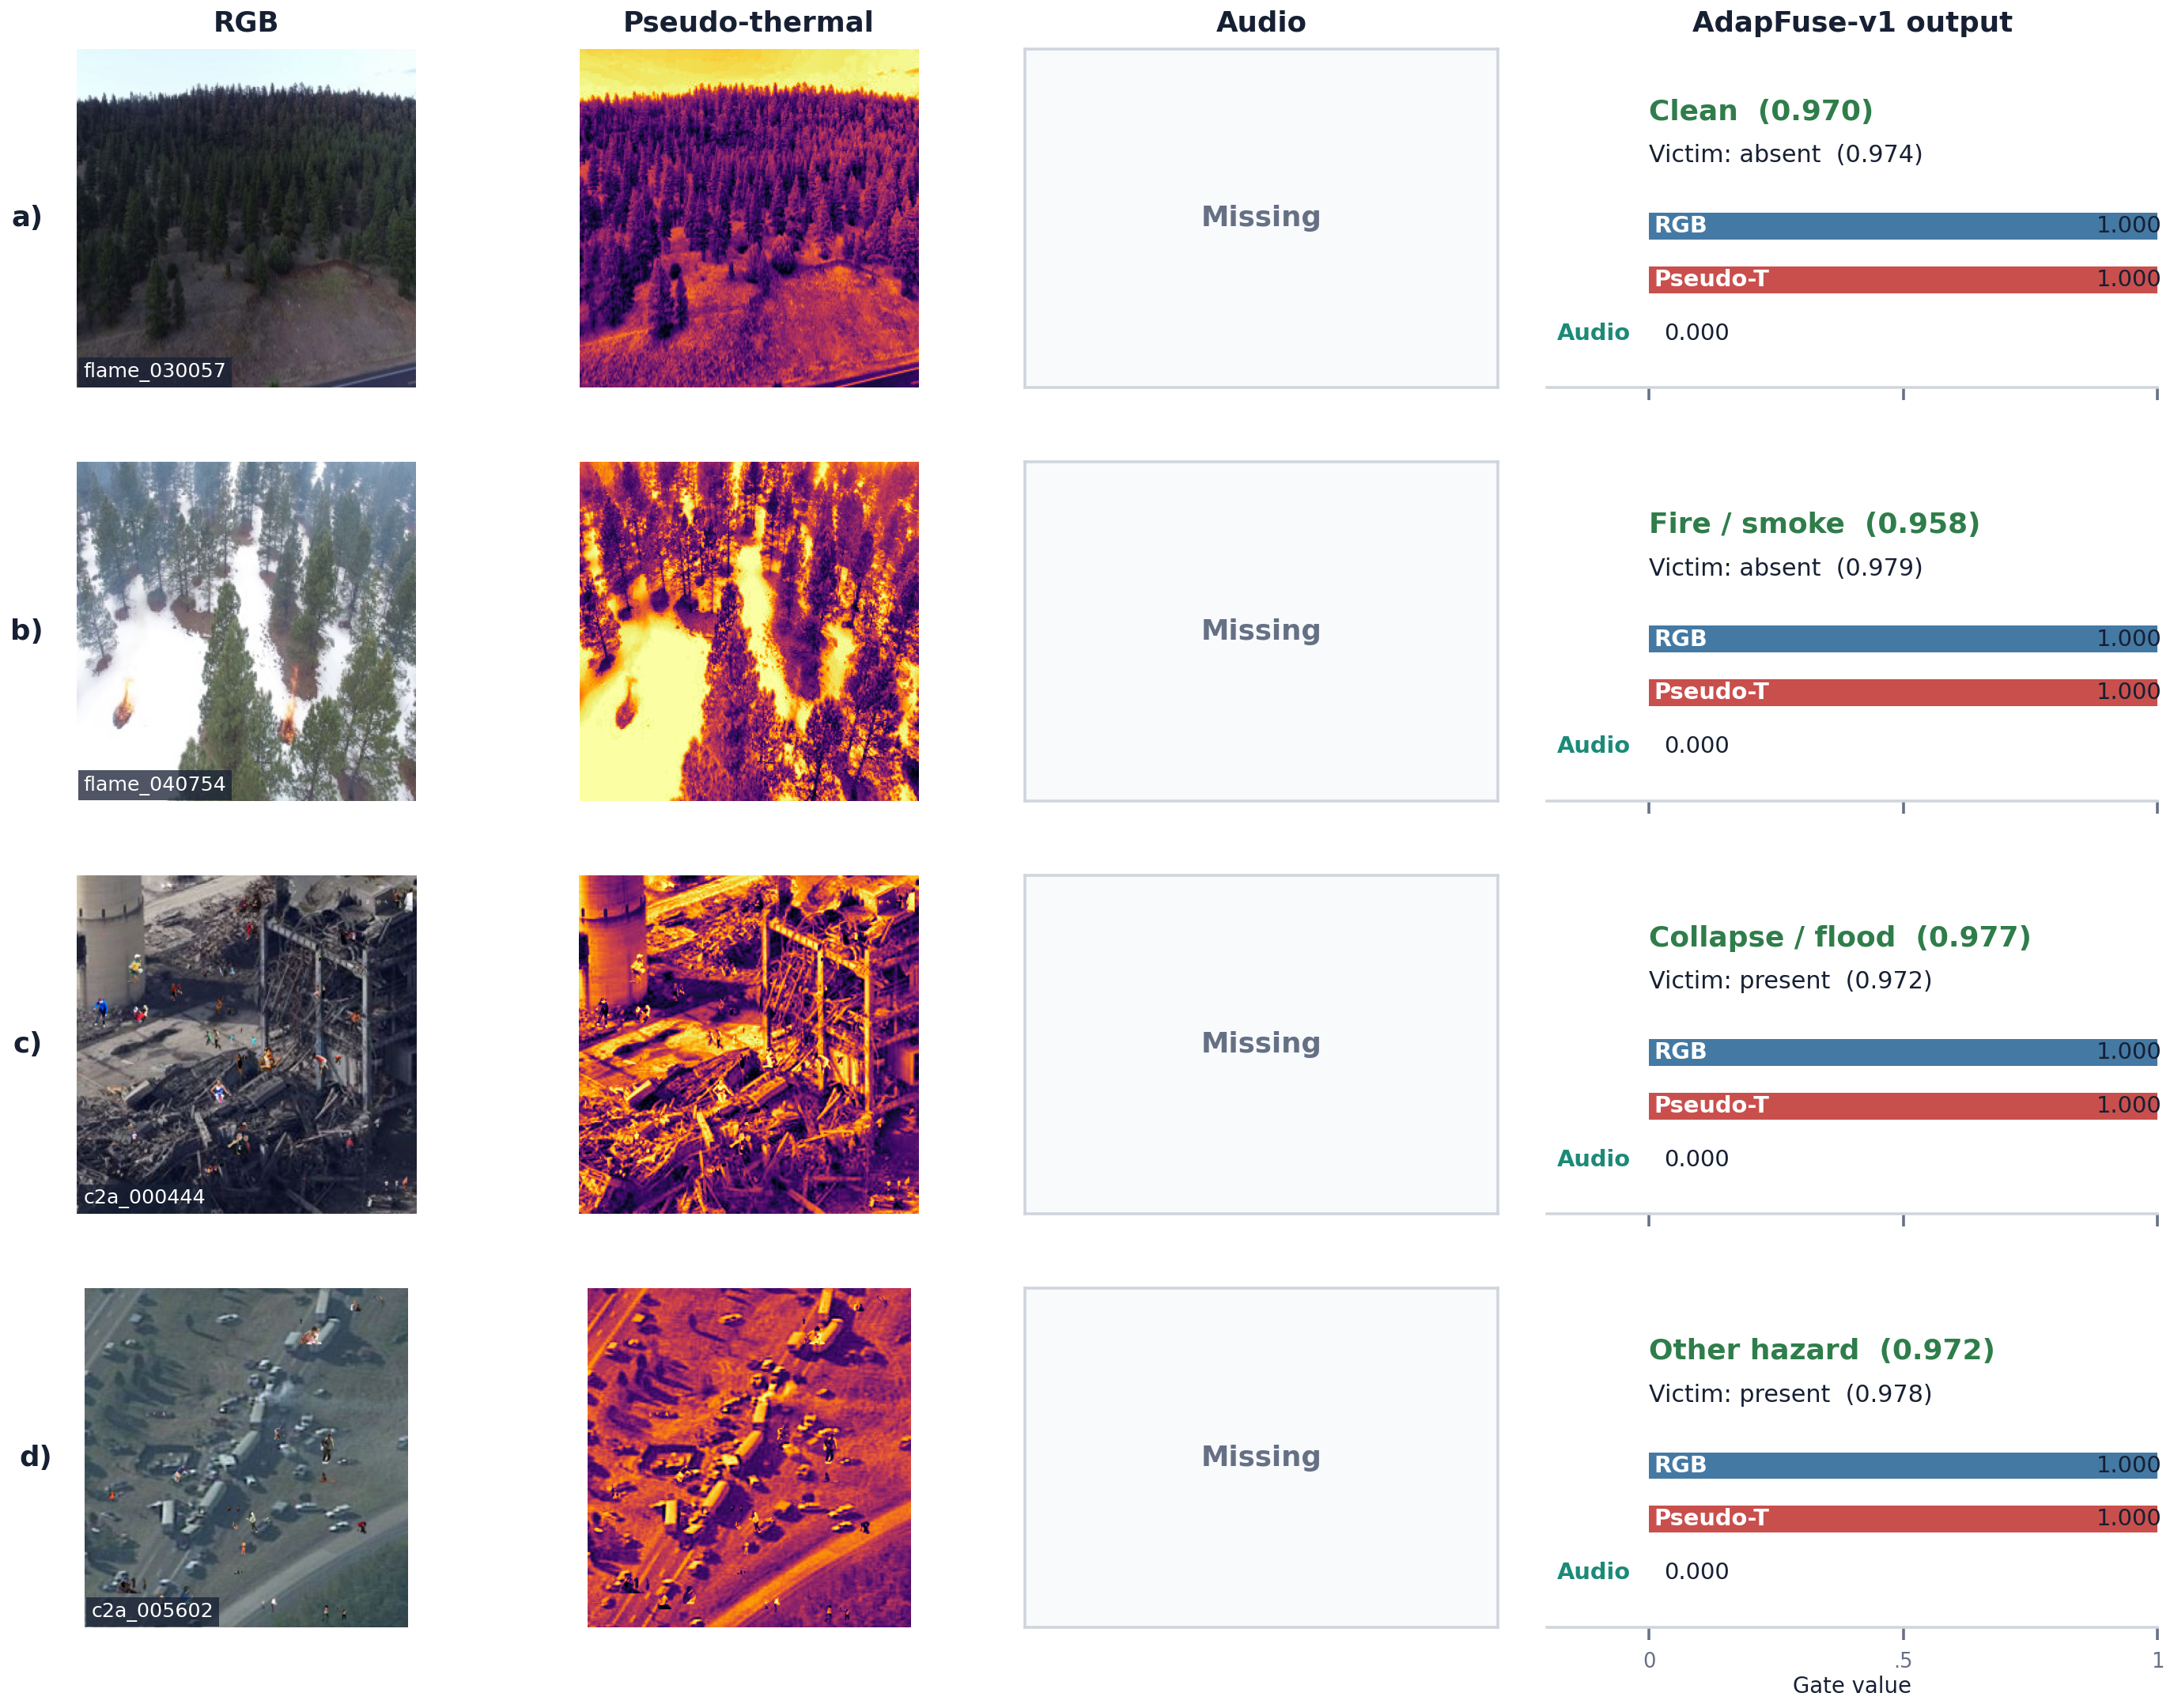
\includegraphics[width=0.8\textwidth]{fig_02_qualitative.png}
\caption[AdapFuse-v1 outputs on four held-out test rows]{AdapFuse-v1 outputs on four held-out test rows: RGB image, pseudo-thermal map, predicted classes and modality gates. None of these rows has audio, so the audio gate is 0; the two image gates are near 1. All four are classified correctly.}
\label{fig:dataset_pipeline}
\end{figure*}

\subsubsection{Dataset Split and Class Distribution}

\paragraph{Raw Split and Class Imbalance}
\label{sec:dataset_split}

The 72{,}997 rows are split into train/validation/test by disaster-label stratification, producing 51{,}097 training, 10{,}949 validation, and 10{,}951 test rows. The split builder does not group by source video, flight, or near-duplicate sequence. Consequently, visually adjacent frames can occur across splits; the test set is held out at row level but is not a strict cross-flight generalization benchmark. A capture-group-aware split was subsequently constructed to measure the size of this effect; it is described and evaluated in Section~\ref{sec:grouped_split}, and all row-level scores in this work should be read alongside it. The raw training split is severely imbalanced: fire/smoke dominates at 46.5\% while collapse/flood and other hazards together account for only 12.5\%.

\paragraph{Two-Stage Class Balancing}

To address this, a two-stage oversampling procedure is applied to the training and validation splits. The test set is \emph{never} resampled; it retains the natural distribution of the collection throughout all experiments.

\textbf{Stage 1: Disaster balance.} Each of the four disaster classes is oversampled to the majority-class count (23{,}746, the fire/smoke count) by sampling with replacement. All synthetic duplicate rows are marked with a synthetic-row indicator; the data loader applies stronger augmentation (additional jitter and masking) to these rows during training to reduce overfitting on duplicated samples.

\textbf{Stage 2: Victim balance.} After disaster balancing, the victim-present class (originally 21.7\% of training) is oversampled proportionally across disaster classes to achieve a 50/50 victim split while preserving the disaster class balance. This produces the \textit{full-balanced} split of 98{,}556 samples (48.2\% synthetic rows).

\paragraph{Stratified Balanced Training Configuration (Resource Constraint)}

Training large suites of multimodal models on the full-balanced split ($\sim$98{,}556 samples) at batch size 16 on a single RTX 5090 (32\,GB VRAM) was estimated at planning time to require approximately 3 hours per run and $\sim$80 hours total. A \textit{Stratified Balanced Training Subset} is therefore derived by applying source-stratified 50\% sampling to each disaster class of the full-balanced split, with a minimum of 5 rows per dataset source to ensure no source is dropped. The result is exactly 12{,}319 rows per disaster class, halving the data per epoch while preserving exact class balance and full source coverage. (Actual logged run times, given below, were longer than this planning estimate.)

\textbf{All twenty-six trained multimodal classification models use the Stratified Balanced Training Configuration.} The grouped-split retraining of AdapFuse-v1 (Section~\ref{sec:grouped_split}) is a separate run outside these twenty-six and was trained without class balancing.

Table~\ref{tab:balancing} summarises the transformation from raw to final training distribution.

\begin{table*}[!t]
\centering
\caption[Raw split vs.\ Stratified Balanced Subset]{Split sizes before and after balancing (training and validation only; test set unchanged).}
\label{tab:balancing}
\resizebox{\textwidth}{!}{%
\begin{tabular}{@{}lrrrrrr@{}}
\toprule
& \multicolumn{2}{c}{\textbf{Raw (original)}} & \multicolumn{2}{c}{\textbf{Full balanced}} & \multicolumn{2}{c}{\textbf{Stratified Balanced (used)}} \\
\cmidrule(lr){2-3} \cmidrule(lr){4-5} \cmidrule(lr){6-7}
\textbf{Subset / Class} & \textbf{Count} & \textbf{\%} & \textbf{Count} & \textbf{\%} & \textbf{Count} & \textbf{\%} \\
\midrule
\textbf{Training total}         & 51{,}097 & n/a    & 98{,}556 & n/a    & \textbf{49{,}276} & n/a \\
\quad Normal / Clean (0)        & 20{,}959 & 41.0\% & 24{,}639 & 25.0\% & 12{,}319          & 25.0\% \\
\quad Fire / Smoke (1)          & 23{,}746 & 46.5\% & 24{,}639 & 25.0\% & 12{,}319          & 25.0\% \\
\quad Collapse / Flood (2)      &  4{,}355 &  8.5\% & 24{,}639 & 25.0\% & 12{,}319          & 25.0\% \\
\quad Other hazard (3)          &  2{,}037 &  4.0\% & 24{,}639 & 25.0\% & 12{,}319          & 25.0\% \\
\quad Victim present (of total) & 11{,}096 & 21.7\% & 49{,}278 & 50.0\% & 24{,}639          & 50.0\% \\
\quad Synthetic (augmented) rows&       0  &  0.0\% & 47{,}459 & 48.2\% & 23{,}696          & 48.1\% \\
\midrule
\textbf{Validation total}       & 10{,}949 & n/a    & 21{,}030 & n/a    & 10{,}516          & n/a \\
\textbf{Test total (held-out)}  & \multicolumn{6}{c}{10{,}951: natural distribution, never resampled} \\
\quad Normal (0)                & \multicolumn{6}{c}{4{,}492 (41.0\%) \quad Fire/Smoke (1): 5{,}089 (46.5\%) \quad Collapse (2): 934 (8.5\%) \quad Other (3): 436 (4.0\%)} \\
\bottomrule
\end{tabular}%
}
\footnotesize{Note: the Stratified Balanced training and validation totals (49{,}276 and 10{,}516) are each 1--2 rows short of an exact half of the full-balanced counts (98{,}556 and 21{,}030) due to per-source rounding under the minimum-5-rows-per-source constraint applied during stratified 50\% sampling.}
\end{table*}

Figure~\ref{fig:dataset_composition} shows the source and label distributions for the dataset.

\begin{figure*}[!t]
\centering
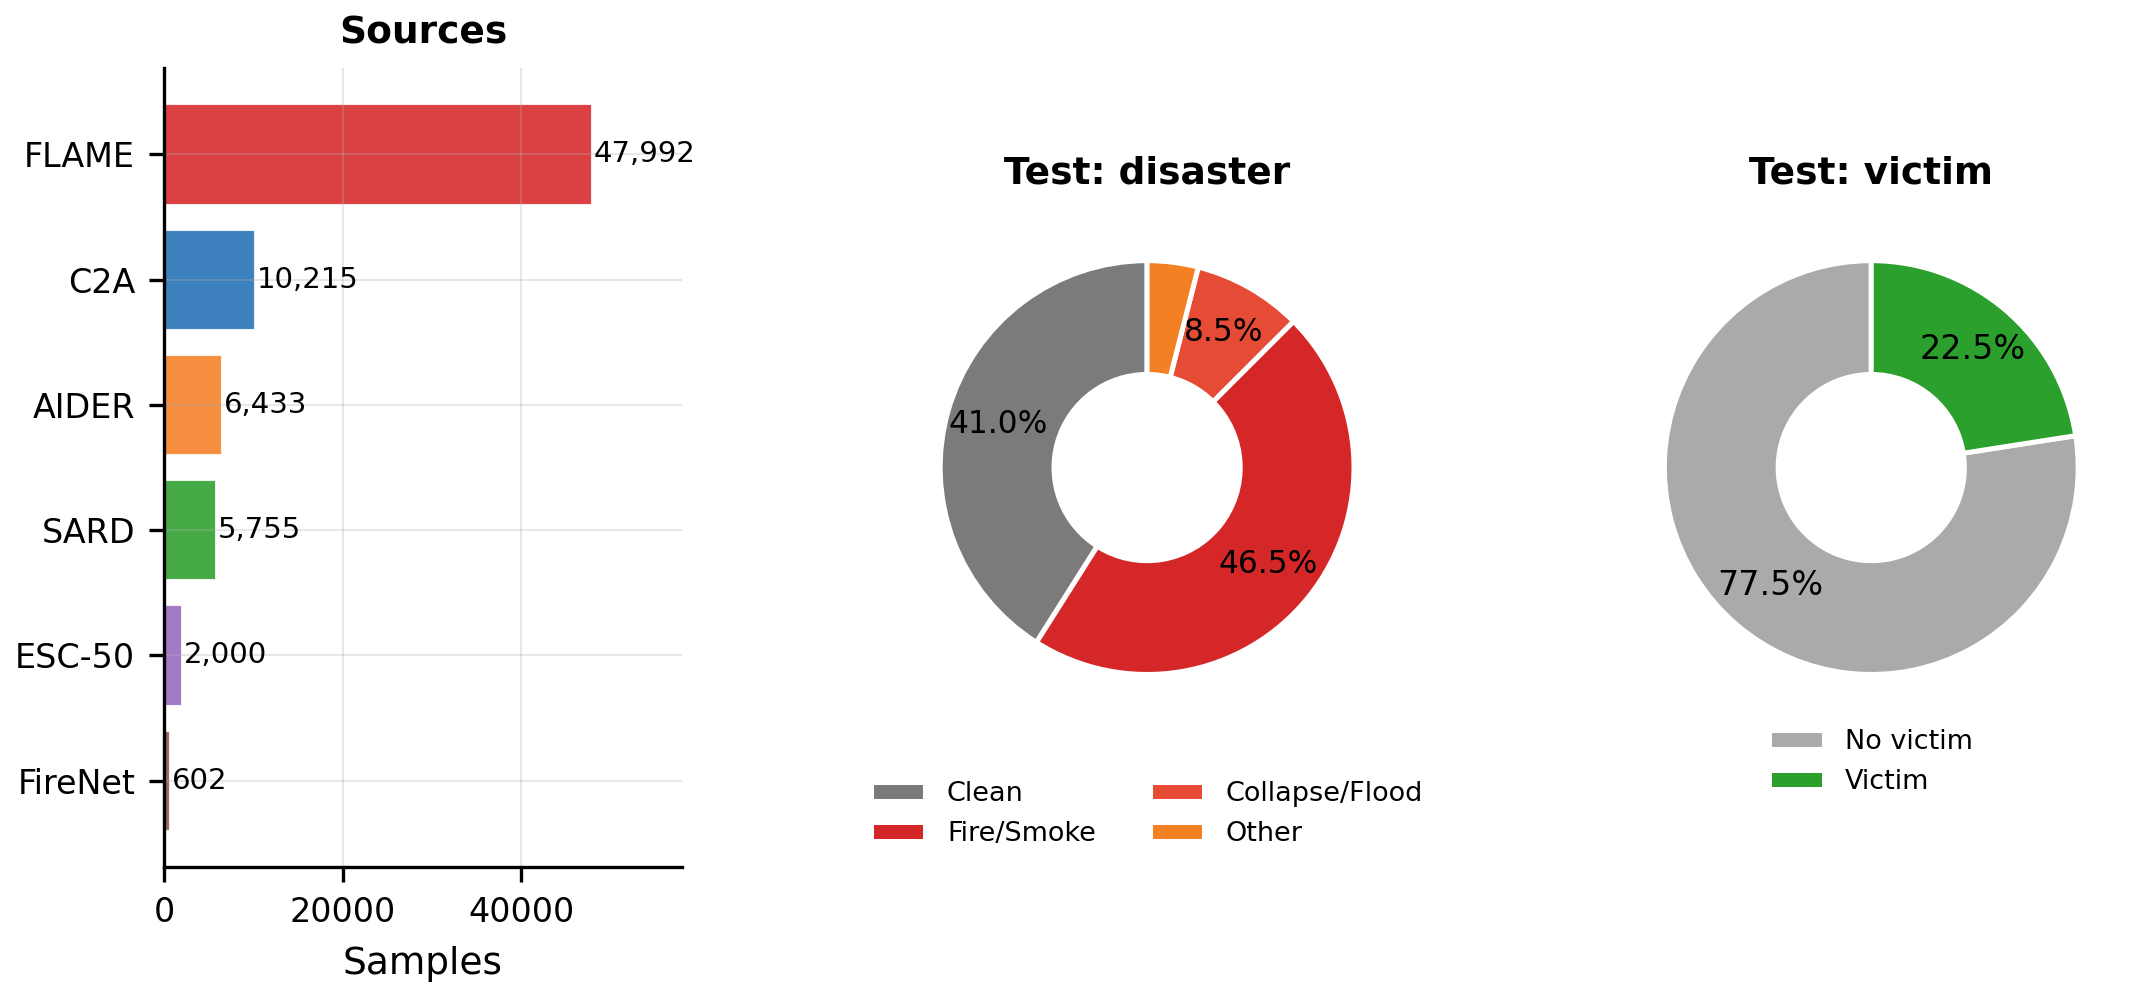
\includegraphics[width=0.8\textwidth]{fig_08_dataset.png}
\caption[Dataset composition]{Dataset composition: 72{,}997 samples from six sources (left) and test-set label distributions for disaster class (centre) and victim presence (right). FLAME supplies 65.7\% of all samples.}
\label{fig:dataset_composition}
\end{figure*}

Figure~\ref{fig:balanced_training} visualises all four aspects of this transformation: disaster class redistribution, victim balance correction, per-source composition, and original-versus-synthetic row breakdown per class.

\begin{figure*}[!t]
\centering
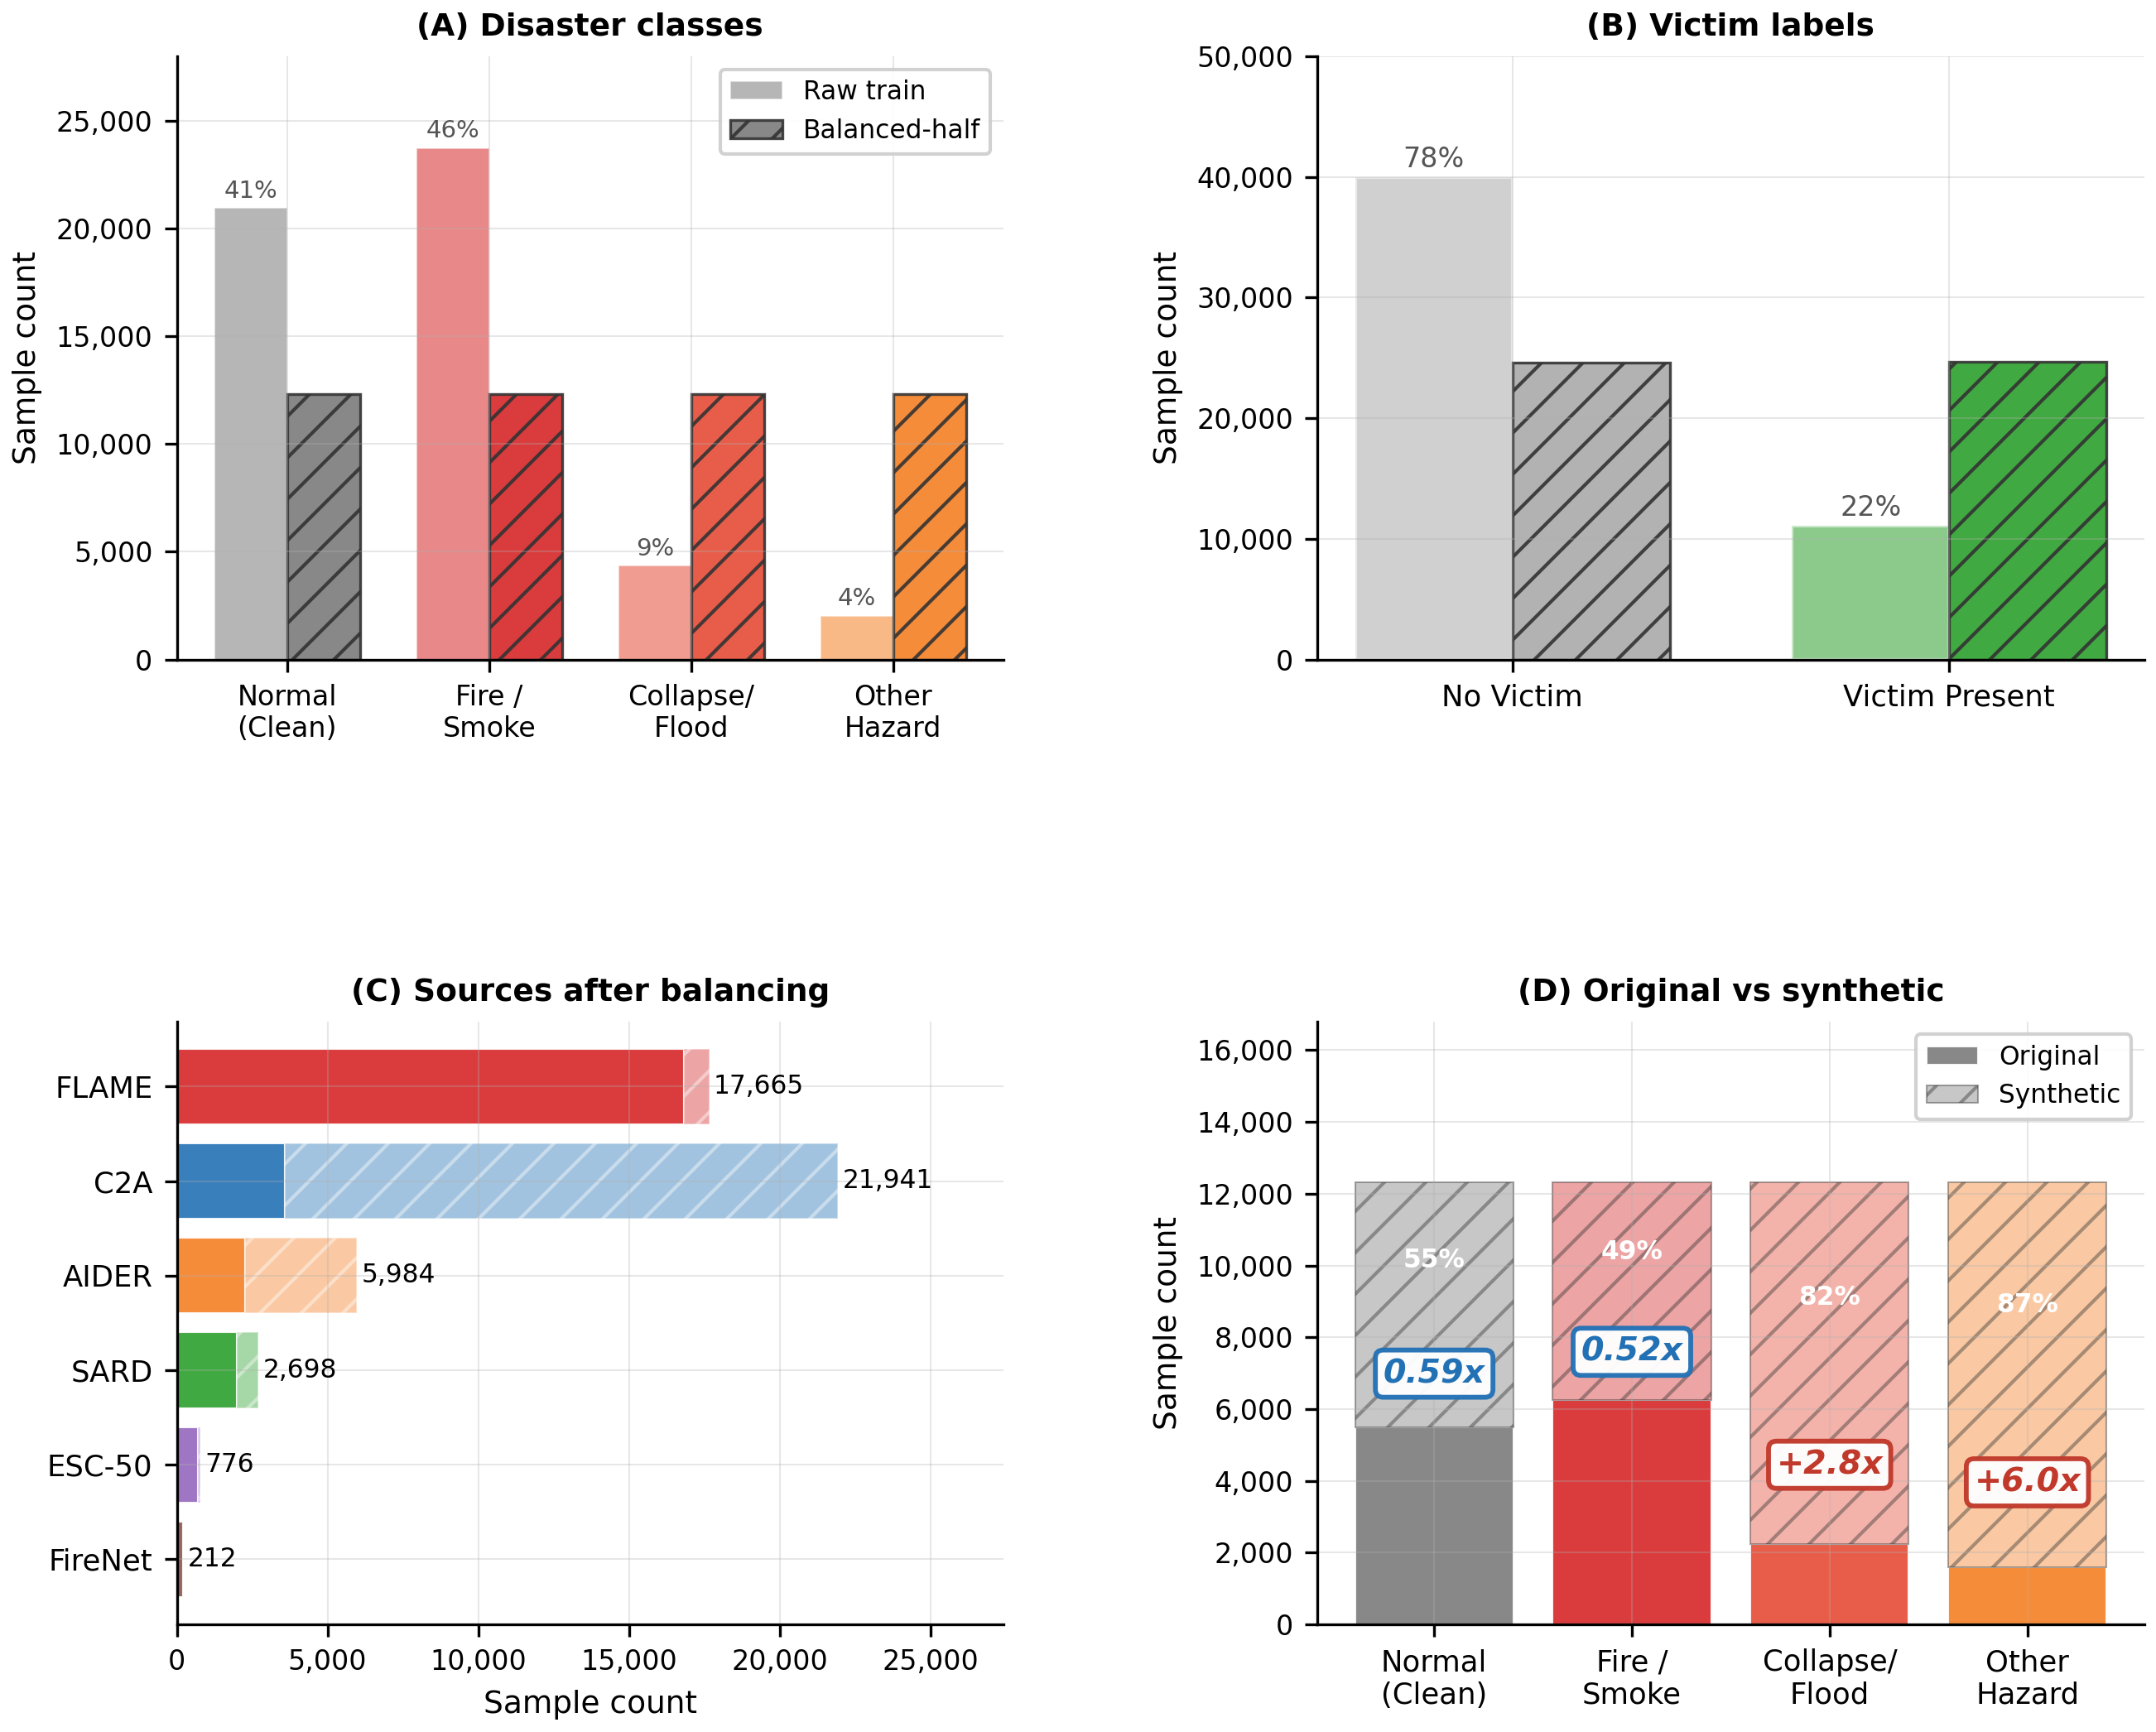
\includegraphics[width=0.8\textwidth]{fig_10_balanced_training.png}
\caption[Stratified Balanced Training Subset]{Stratified Balanced Training Subset (49{,}276 samples, 48.1\% synthetic duplicates). (A) Disaster classes balanced to 25\% each. (B) Victim presence balanced to 50/50. (C) Source mix; all six sources kept (hatched: synthetic). (D) Original vs.\ synthetic rows per class (red: oversampled; blue: downsampled).}
\label{fig:balanced_training}
\end{figure*}

\noindent\textbf{Note on per-source composition.} C2A is the primary source for the Collapse/Flood and Other hazard classes, which are oversampled 2.8$\times$ and 6.0$\times$ respectively (Figure~\ref{fig:balanced_training}D) to reach the 12{,}319-per-class target. Because oversampling is applied at the class level rather than the source level, C2A's row count in the Stratified Balanced Training Subset (21{,}941) exceeds its entire raw sample count (10{,}215, Table~\ref{tab:dataset_sources}); this reflects heavy within-class duplication of C2A's minority-class rows, not an error in source accounting.

\noindent\textbf{Implication for metrics.} Because the test set retains the natural imbalanced distribution, \textit{macro F1} is reported as the primary metric throughout Chapter~5. Macro F1 weights each class equally regardless of frequency, correctly penalising a model that ignores the rare collapse/other classes. Accuracy (which weights by sample frequency) is reported as a secondary metric. The 8.5\% collapse and 4.0\% other classes together constitute only 12.5\% of test samples, meaning accuracy can remain above 98\% even when the model entirely fails on those classes.

\subsubsection{Data Preprocessing}

\textbf{RGB:} Images are resized to 224$\times$224 and normalized to ImageNet mean and standard deviation. The base training transform includes random horizontal flip, colour jitter, Gaussian blur, and rotation. Although the loader implements explicit smoke, low-light, motion-blur, and noise functions, the reported base configuration sets no corruption\_type; therefore its corruption\_prob=0.3 does not activate those explicit corruptions. For reproducibility: every base training run reported in Chapter~5 (including Tables~\ref{tab:main_results}, \ref{tab:adaptfuse_extended} and \ref{tab:ablation_results}) used no synthetic corruption augmentation; the corruption sweeps appear only in the offline evaluation of Section~\ref{sec:robustness_stress_test}.

\textbf{Pseudo-thermal:} RGB-derived maps are read in grayscale, resized to 224$\times$224, and z-score normalized. The classification loader does not apply CLAHE in the reported AdapFuse-v1 run, and these intensity values are not radiometric temperatures.

\textbf{Audio:} Two-second clips at 16 kHz are transformed into normalized log-mel spectrograms (64 frequency bins, 63 time frames). The current classification loader does not apply spectral subtraction or SpecAugment. Rotor-noise corruption exists as an evaluation option but is not activated by the base training configuration without an explicit corruption type.

\textbf{Missing modality simulation:} During training, one sensor is randomly dropped (zero-filled) with probability 0.2 per sample, exposing each model to missing inputs during training.

\subsection{Preliminary Design: Six Fusion Architectures}

Six fusion designs are implemented and compared to evaluate the contribution of each design choice. Table~\ref{tab:designs} summarises the six designs; Figure~\ref{fig:design_comparison} illustrates the structural differences. For every design, including our own, the table lists the principal limitation observed in this study rather than only the intended benefit.

\begin{table*}[!t]
\centering
\caption[Summary of the six fusion designs]{Summary of the six fusion designs. \textit{Limitation}: main weakness observed in our experiments.}
\label{tab:designs}
\resizebox{\textwidth}{!}{%
\begin{tabular}{@{}clp{4.6cm}p{5.2cm}@{}}
\toprule
\textbf{Design} & \textbf{Name} & \textbf{Approach} & \textbf{Limitation} \\
\midrule
A1 & RGB-only          & MobileNetV3-Small; 576-dim $\to$ FC classifier & No thermal or audio cue; vulnerable under heavy smoke and low-light conditions \\
A2 & Pseudo-thermal-only& ResNet-18 (1-channel); 512-dim $\to$ FC classifier & No colour cue; lower spatial resolution \\
A3 & Audio-only        & 2D-CNN on log-mel (32$\to$64$\to$128 filters) & Label-matched ESC-50 clips; rotor noise not tested \\
B  & Early Fusion      & 5-channel input (RGB 3ch + Thermal 1ch + Audio resized 1ch) processed by one shared ResNet-18 & One backbone handles all sensor types; loses modality-specific features \\
C  & Late Fusion       & Three independent models produce class probabilities; learned weighted average & Sensors never share intermediate features \\
D  & Intermediate (Fixed) & Per-sensor backbone $\to$ 192-dim projection $\to$ concatenate $\to$ MLP & All sensors weighted equally regardless of quality \\
\midrule
E  & \textbf{AdapFuse-v1 (ours)} & Design D + RUE reliability weighting + cross-modal attention + NuisanceAwareHead & RUE gates unsupervised and saturated (static per-modality weights); single-step GRU; nuisance head unsupervised; only +0.05\,pp macro-F1 over D \\
F  & \textbf{AdapFuse-v2 (ours, KD)} & AdapFuse-v1 teacher $\to$ knowledge distillation $\to$ half-width student (proj\_dim=96) & Inherits all limitations of E; only 4.9\% fewer parameters (backbones unchanged); on-device latency not measured \\
\bottomrule
\end{tabular}%
}
\end{table*}

\noindent Each unimodal baseline is also trained with two alternative backbones, giving three per modality: EfficientNet-B0 and MobileViT-XXS for RGB and for 1-channel pseudo-thermal, and a CNN6-style encoder and a GDBlock variant of the AudioCNN for audio. Section~\ref{sec:unimodal_backbones} reports these runs, which allow each fused model to be compared with a unimodal model that uses the same backbone.

\noindent\textbf{Limitations of the proposed designs.} Designs E and F are held to the same standard as the baselines. For AdapFuse-v1, three of its four added components do not yet behave as their names suggest. (i)~The RUE receives no degradation targets, so its gates converge to saturated, input-independent values and act as a learned static weighting per modality, not a dynamic reliability estimate (Section~\ref{sec:robustness_stress_test}). (ii)~The GRU runs on a sequence of length one and therefore provides no temporal smoothing. (iii)~The NuisanceAwareHead receives no nuisance labels, so its loss is zero during training. The measured gain over the fixed-weight Design D is correspondingly small: +0.05\,pp combined macro-F1, together with a 2.9$\times$ lower focal test loss (Figure~\ref{fig:design_comparison}). AdapFuse-v2 inherits these properties. Because distillation halves only the projection width while the backbones stay unchanged, it removes just 4.9\% of the parameters (12.94M $\to$ 12.30M), and its deployment benefit has not been verified on embedded hardware. Accordingly, we present E and F as an architecture whose adaptive components are \emph{implemented but not yet validated}. Sections~\ref{sec:robustness_stress_test} and~\ref{sec:grouped_gates} give the supporting evidence, and the concluding chapter outlines the supervision needed to validate them.

\begin{figure*}[!t]
\centering
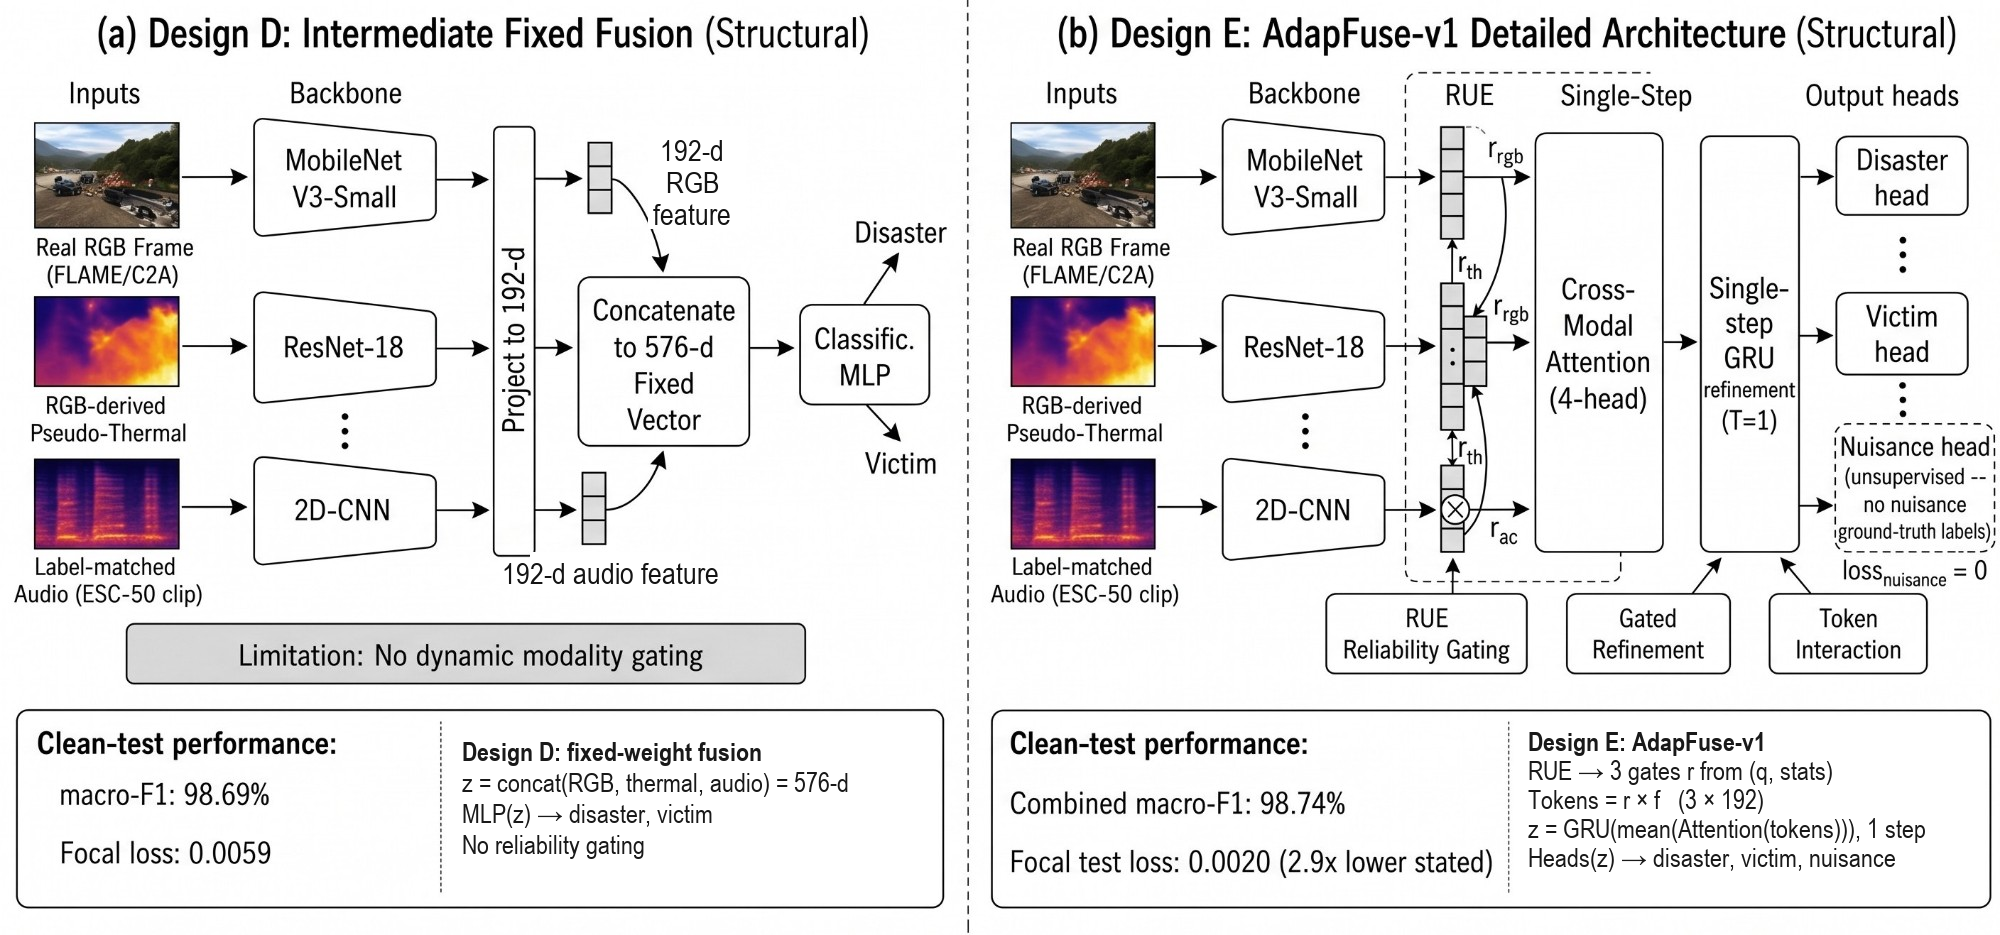
\includegraphics[width=0.8\textwidth]{4.5.png}
\caption[Design D vs.\ Design E (AdapFuse-v1)]{Design D (fixed fusion) vs.\ Design E (AdapFuse-v1). AdapFuse-v1 gains 0.05\,pp combined macro-F1 and has a 2.9$\times$ lower focal test loss. Its GRU is single-step and its nuisance head is unsupervised.}
\label{fig:design_comparison}
\end{figure*}

Figure~\ref{fig:data_provenance} summarises what our metadata actually supply for each modality, and which supervision signals assumed by the architecture are absent from it.

\begin{figure*}[!t]
\centering
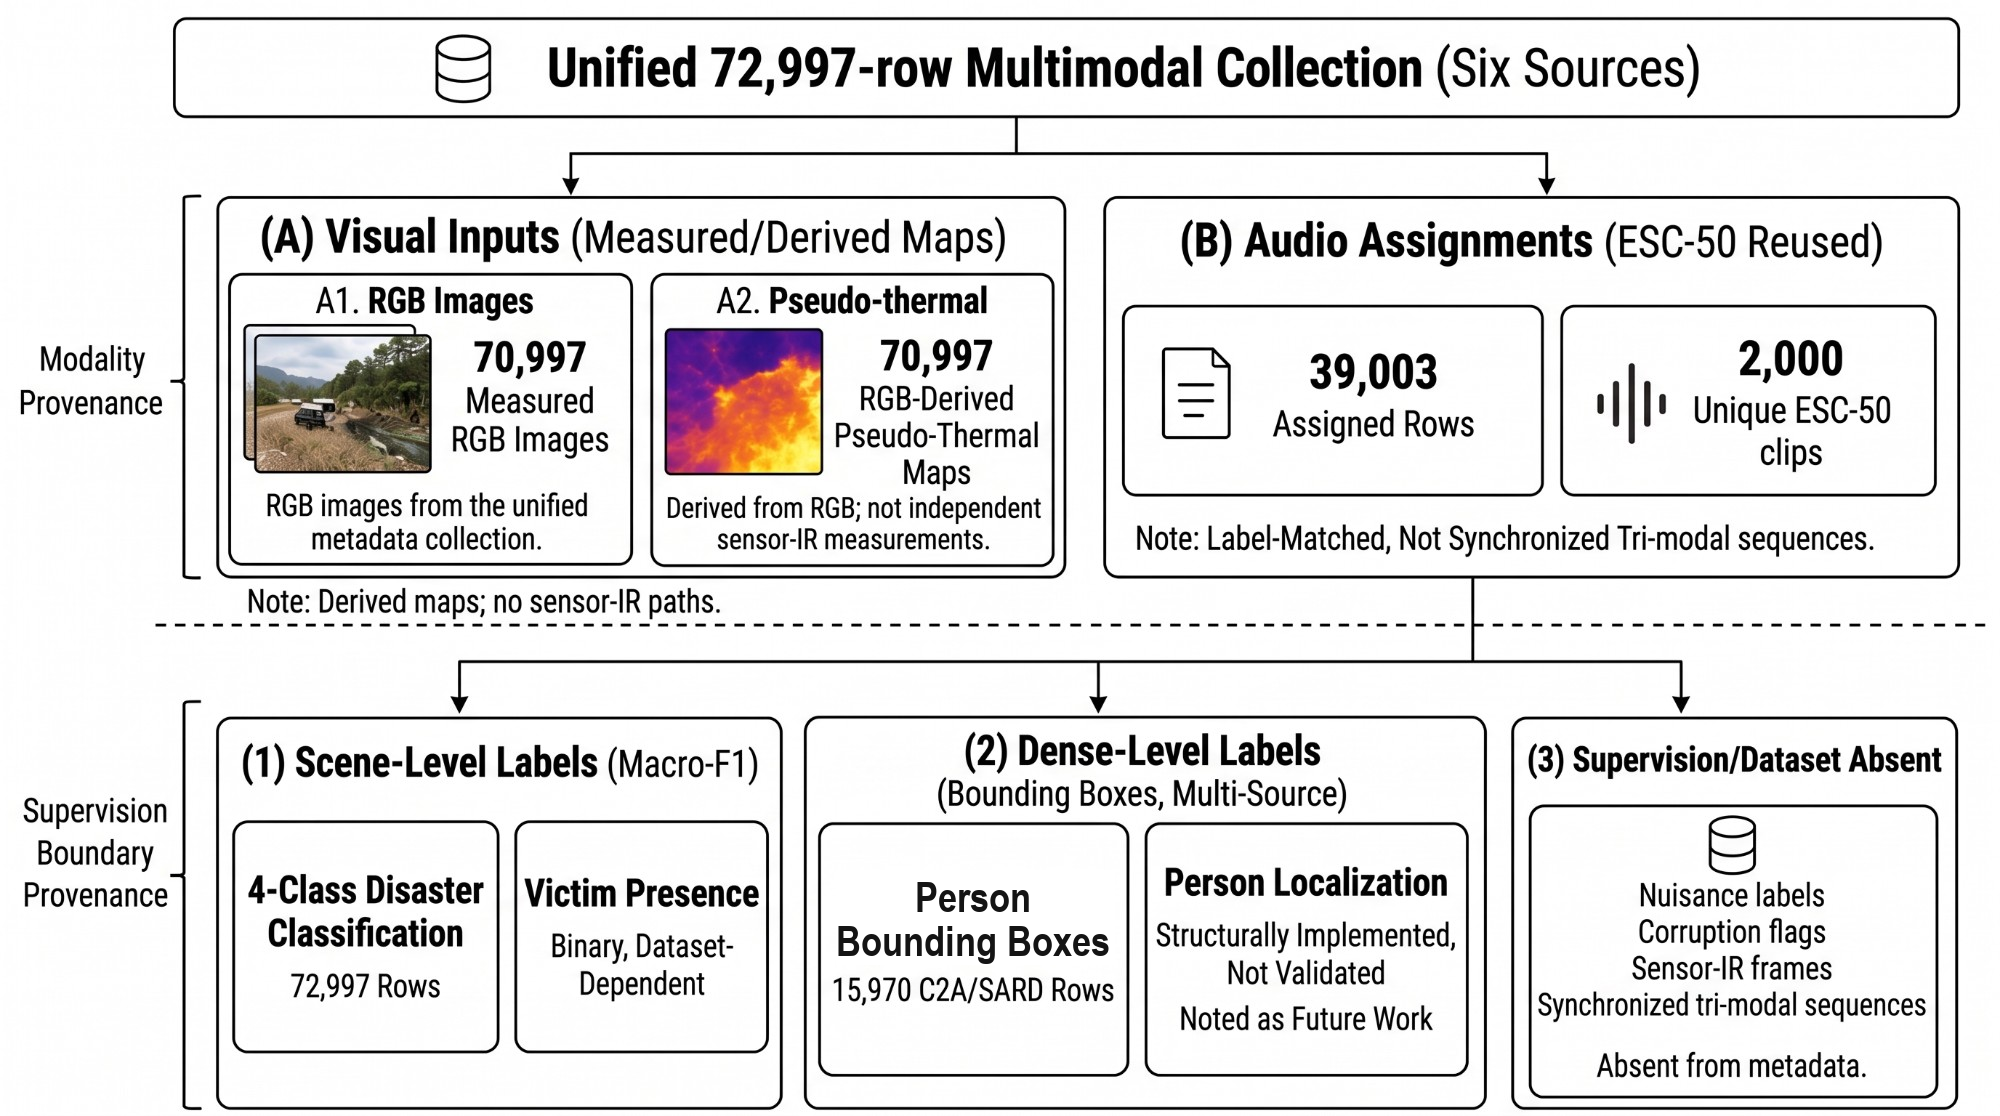
\includegraphics[width=0.8\textwidth]{4.6.png}
\caption[Data provenance and supervision boundary]{Data provenance and supervision boundary. Pseudo-thermal maps are derived from RGB, and audio is label-matched (2{,}000 ESC-50 clips reused across 39{,}003 rows), not synchronized. Nuisance labels, corruption flags and sensor-IR frames are absent.}
\label{fig:data_provenance}
\end{figure*}

\subsection{AdapFuse-v1: Detailed Architecture}

\subsubsection{Modality-Specific Encoders}

Each sensor has a dedicated lightweight backbone producing a 192-dimensional projected feature:

\begin{itemize}
    \item \textbf{RGB:} MobileNetV3-Small~\cite{howard2019mobilenetv3} pretrained on ImageNet. The 576-dim pooled output of its final $1\times1$ convolution is projected to 192 dimensions via a linear layer. Compute: $\approx$0.06 GMACs per frame (Table~\ref{tab:backbone_candidates}).
    \item \textbf{Pseudo-thermal:} ResNet-18~\cite{he2016deep} adapted for single-channel input (pretrained first-layer weights summed across the RGB channels). The 512-dim global average-pooled output is projected to 192 dimensions. All populated thermal paths in our metadata are RGB-derived maps; no sensor-IR inputs are evaluated.
    \item \textbf{Audio:} A three-layer 2D-CNN on the 64$\times$63 log-mel spectrogram (filter progression 32$\to$64$\to$128). Global average pooling produces a 128-dim vector projected to 192 dimensions.
\end{itemize}

Each backbone additionally outputs a 16-dimensional \textit{quality token}, a learned linear projection of its penultimate activations intended to summarise how distinctive and high-confidence the backbone's internal representation is.

\subsubsection{Reliability and Uncertainty Estimator (RUE)}

The RUE is a two-layer MLP that receives the three 16-dim quality tokens plus a 6-dim vector of feature statistics (per-modality mean and variance of the 192-dim features). It outputs three sigmoid gates $r_i \in [0,1]$ and three uncertainty values. In the reported training path, degradation targets are passed as None; the gates are therefore shaped indirectly by task loss and a variance regularizer rather than calibrated against sensor-quality ground truth:

\begin{multline}
    [r_{rgb}, r_{th}, r_{au}] = \\ \sigma\!\left(W_2 \cdot \text{ReLU}(W_1 \cdot [\mathbf{q}_{rgb}\|\mathbf{q}_{th}\|\mathbf{q}_{au}\|\mathbf{s}] + b_1) + b_2\right)
\end{multline}

where $\mathbf{q}_i \in \mathbb{R}^{16}$ are quality tokens, $\mathbf{s} \in \mathbb{R}^6$ are feature statistics, and $\sigma$ is the sigmoid function. Each modality's 192-dim feature vector is multiplied by its reliability score before entering the attention module, so that, by design, a modality with a low gate contributes less to the fused representation.

\textbf{Limitation.} Because no degradation labels or corruption flags are supplied (degradation\_targets=None), nothing in training ties a gate value to sensor quality. In our row-level model, the RGB and pseudo-thermal gates are saturated at $\approx$1.0 on every row that has the input and the audio gate is $\approx$0.011, and none of them moves across the synthetic corruption sweeps (Section~\ref{sec:robustness_stress_test}); the grouped-split retraining converges to different, equally saturated gates (Section~\ref{sec:grouped_gates}). The RUE therefore acts in these experiments as a learned, run-dependent on/off weighting per modality, not as a dynamic reliability estimator. Supervising it with explicit degradation targets and testing gate response against measured degradation is future work.

\subsubsection{Cross-Modal Attention Fusion}

The three reliability-weighted features are stacked as tokens $\mathbf{T} \in \mathbb{R}^{3 \times 192}$ and processed by a multi-head cross-attention module~\cite{vaswani2017attention} with 4 heads. This allows each modality to attend to context from the other two, learning complementary cross-sensor patterns (e.g.\ RGB flame-region attending to the thermal hotspot token):

\begin{equation}
    \hat{\mathbf{T}} = \text{MultiHead}(\mathbf{T}, \mathbf{T}, \mathbf{T})
\end{equation}

The mean-pooled output $\hat{f} = \text{mean}(\hat{\mathbf{T}}) \in \mathbb{R}^{192}$ is passed through a GRU (hidden size 192). The current dataset provides independent frames and the implementation calls the GRU on fused.unsqueeze(1) without passing a hidden state, so sequence length is one and each sample starts from a zero state; nothing is carried between frames. It is therefore a gated nonlinear refinement layer in these experiments; temporal smoothing across frames is not evaluated.

\subsubsection{NuisanceAwareHead}

The NuisanceAwareHead defines logits for:
\begin{enumerate}
    \item \textbf{Disaster class} (0=clean, 1=fire/smoke, 2=collapse/flood, 3=other), the primary task
    \item \textbf{Victim presence} (binary), the secondary task
    \item \textbf{Nuisance type} (5-class: clean signal, solar heating, RGB false fire, audio false alarm, partial occlusion), an architectural auxiliary branch
\end{enumerate}

In our trainer, nuisance\_gt=None; consequently the nuisance loss is zero and this branch is not supervised in the reported checkpoints. At inference only disaster and victim logits are reported. The observed false-positive rate must therefore be attributed to the trained scene classifier as a whole, not specifically to nuisance supervision. Our dataset contains no nuisance-category labels, so the nuisance branch is an unvalidated architectural provision rather than a demonstrated contribution; validating it would require nuisance-labelled false-alarm data and a comparison of false-positive rates with and without nuisance supervision.

\subsubsection{Visual and Audio Backbone Variants}

In addition to the baseline encoders, several architectural variants were implemented:
\begin{itemize}
    \item \textbf{EfficientNet-B0 Visual Backbones:} Replacing MobileNetV3-Small or ResNet-18 with EfficientNet-B0~\cite{tan2019efficientnet}, which leverages compound scaling across network depth, width, and resolution to capture fine-grained spatial and thermal signatures.
    \item \textbf{MobileViT-XXS Hybrid Transformer:} Incorporating MobileViT-XXS~\cite{mehta2022mobilevit}, combining MobileNet inverted residual blocks with lightweight Transformer self-attention to capture long-range aerial disaster scene dependencies at a small parameter budget (edge-device memory use is not measured here).
    \item \textbf{PANNS-CNN6-style Audio Backbone:} A 4-block convolutional network with the channel widths of PANNs CNN6~\cite{kong2020panns} (64--512), producing 512-dimensional acoustic representations. Our implementation uses $3\times3$ kernels, whereas the released AudioSet checkpoint uses $5\times5$ kernels, so none of the checkpoint's convolution weights load (only 8 of 20 tensors, all batch-normalisation parameters). This encoder is therefore effectively trained from scratch, not an AudioSet transfer.
    \item \textbf{AudioCNN-GD Backbone:} A multi-scale dilated convolutional architecture employing parallel dilation rates ($d \in \{1, 3, 5\}$) to capture both transient bursts and sustained frequency patterns, a design aimed at rotor-noise environments (not tested here with measured rotor noise).
\end{itemize}

\subsubsection{Backbone Selection Rationale}
\label{sec:backbone_selection}

The encoders were chosen against four criteria derived from the target payload (Section~\ref{sec:tech_requirements}: embedded GPU with TDP $\leq$15\,W, $\geq$10 FPS, INT8 inference for all encoders):
\begin{enumerate}
    \item \textbf{Pretrained weights.} Each visual encoder must have public ImageNet weights, and the audio encoder should have AudioSet weights, because every training source is small relative to these corpora.
    \item \textbf{Per-stream compute budget.} Three encoders run on every frame, so each is limited to about 1\,GMAC and 5\,M parameters at $224\times224$. This budget is a design choice, not a measured limit of a specific edge device.
    \item \textbf{Accuracy within the budget.} Among candidates inside the budget, those with the highest ImageNet top-1 are preferred.
    \item \textbf{Family diversity.} The three visual candidates cover three design families (a hand-designed mobile CNN, a compound-scaled CNN and a CNN--Transformer hybrid), so a backbone ablation tests different inductive biases, not three sizes of one network.
\end{enumerate}

Table~\ref{tab:backbone_candidates} applies these criteria to thirteen visual candidates. Parameters, MACs and training memory were measured by us with a single benchmark script; ImageNet top-1 is the value published with each set of weights. These quantities are properties of each network rather than of the GPU. Latency on the RTX 5090 (32\,GB VRAM) training workstation would not predict on-board UAV latency, so it is not used as a selection criterion.

\begin{table*}[!t]
\centering
\caption[Visual backbone candidates]{Visual backbone candidates (feature extractor only, $3\times224\times224$ input). Mem.: peak training memory at batch 16. Shaded rows fit the budget ($\leq$1\,GMAC, $\leq$5\,M params). $^\dagger$Lower bound. $^\ddagger$From torchvision metadata. $^\ast$Pseudo-thermal only; over budget.}
\label{tab:backbone_candidates}
\resizebox{\textwidth}{!}{%
\begin{tabular}{@{}llcccc l@{}}
\toprule
\textbf{Backbone} & \textbf{Family} & \textbf{Params (M)} & \textbf{GMACs} & \textbf{Top-1 (\%)} & \textbf{Mem.\ (MB)} & \textbf{Decision} \\
\midrule
\rowcolor{gray!12} MobileNetV3-Small~\cite{howard2019mobilenetv3} & Mobile CNN & 0.93 & 0.06 & 67.7 & 151 & \textbf{Selected} \\
\rowcolor{gray!12} ShuffleNetV2-1.0$\times$ & Mobile CNN & 1.25 & 0.14 & 69.4 & 194 & Not used \\
\rowcolor{gray!12} MobileNetV3-Large~\cite{howard2019mobilenetv3} & Mobile CNN & 2.97 & 0.21 & 74.0 & 404 & Not used \\
\rowcolor{gray!12} MobileNetV2 & Mobile CNN & 2.22 & 0.30 & 71.9 & 655 & Not used \\
\rowcolor{gray!12} MobileViT-XXS~\cite{mehta2022mobilevit} & Hybrid & 0.95 & 0.30$^\dagger$ & 69.0 & 414 & \textbf{Selected} \\
\rowcolor{gray!12} EfficientNet-B0~\cite{tan2019efficientnet} & Scaled CNN & 4.01 & 0.39 & 77.7 & 779 & \textbf{Selected} \\
EfficientNet-B3~\cite{tan2019efficientnet} & Scaled CNN & 10.70 & 0.96 & 82.0 & 1{,}546 & Over (params) \\
MobileViT-S~\cite{mehta2022mobilevit} & Hybrid & 4.94 & 1.52$^\dagger$ & 78.4 & 1{,}218 & Over (MACs) \\
ResNet-18~\cite{he2016deep} & CNN & 11.18 & 1.81 & 69.8 & 451 & \textbf{Selected}$^\ast$ \\
ResNet-50~\cite{he2016deep} & CNN & 23.51 & 4.09 & 76.1 & 1{,}152 & Over (MACs) \\
ConvNeXt-Tiny & CNN & 27.82 & 4.46 & 82.5 & 1{,}450 & Over (MACs) \\
Swin-T & ViT & 27.52 & 4.49 & 81.5 & 1{,}591 & Over (MACs) \\
ViT-B/16 & ViT & 85.80 & 17.56$^\ddagger$ & 81.1 & 2{,}628 & Over (MACs) \\
\bottomrule
\end{tabular}%
}
\end{table*}

\textbf{Visual encoders.} MobileNetV3-Small has the lowest computational cost among the evaluated candidates (0.06\,GMACs) and is the default RGB encoder of every fused model. EfficientNet-B0 has the highest ImageNet accuracy inside the budget (77.7\%), and MobileViT-XXS is the only CNN--Transformer hybrid inside it. The other in-budget candidates were not trained: each costs more MACs than MobileNetV3-Small and has a lower top-1 than EfficientNet-B0, so it lies inside the cost--accuracy range the three selected networks already cover. Every candidate above 1\,GMAC was rejected; the larger models (ResNet-50, ConvNeXt-Tiny, Swin-T, ViT-B/16) need 4--18$\times$ the budget per stream while gaining at most 4.8 top-1 points over EfficientNet-B0.

\textbf{Pseudo-thermal encoder.} ResNet-18 is the exception: at 1.81\,GMACs and 11.2\,M parameters it is over budget. It was kept as the A2 baseline because single-channel adaptation of a pretrained ResNet by summing first-layer weights is a common transfer baseline for grey-scale and thermal imagery. The two in-budget replacements are tested directly: both EfficientNet-B0 and MobileViT-XXS outperform it on the pseudo-thermal stream with 2.8--11.8$\times$ fewer parameters (Table~\ref{tab:unimodal_thermal}).

\begin{table*}[!t]
\centering
\caption[Audio backbone candidates]{Audio backbone candidates ($1\times64\times63$ log-mel input). Lower rows are full-network figures from Kong et al.~\cite{kong2020panns}, shown for scale.}
\label{tab:audio_candidates}
\resizebox{\textwidth}{!}{%
\begin{tabular}{@{}lccccl@{}}
\toprule
\textbf{Backbone} & \textbf{Params (M)} & \textbf{GMACs} & \textbf{AudioSet mAP} & \textbf{Train mem.\ (MB)} & \textbf{Decision} \\
\midrule
AudioCNN (from scratch) & 0.09 & 0.037 & -- & 48 & \textbf{Selected} \\
AudioCNN + GDBlock & 0.06 & 0.022 & -- & 58 & \textbf{Selected} \\
CNN6-style encoder ($3\times3$)$^\ast$ & 1.55 & 0.213 & -- & 102 & \textbf{Selected} \\
\midrule
PANNs CNN6 (reported)~\cite{kong2020panns} & 4.8 & -- & 0.343 & -- & Reference \\
PANNs CNN10 (reported)~\cite{kong2020panns} & 5.2 & -- & 0.380 & -- & Over (params) \\
PANNs CNN14 (reported)~\cite{kong2020panns} & 80.8 & -- & 0.431 & -- & Over (params) \\
\bottomrule
\multicolumn{6}{@{}l}{\footnotesize $^\ast$Intended as PANNs CNN6 transfer, but the AudioSet convolution weights ($5\times5$) do not match its $3\times3$ kernels and are not loaded.}
\end{tabular}%
}
\end{table*}

\textbf{Audio encoders.} The three audio encoders cover training from scratch (AudioCNN), a cheaper multi-scale variant (GDBlock) and a wider CNN6-style encoder. The CNN6-style encoder was meant to test AudioSet transfer, but because of the kernel mismatch described above it was trained without pretrained convolution weights, so this thesis does not test AudioSet transfer. Larger audio networks such as PANNs CNN14 are about 16 times over the parameter budget. Because the audio in this corpus is label-matched ESC-50 rather than synchronised UAV audio, a larger audio encoder would not address the main limitation of the audio stream (Section~\ref{sec:unimodal_backbones}).

\textbf{Scope of the selection.} This procedure selects backbones by cost and published accuracy. The selected backbones were then trained end-to-end inside the AdapFuse-UAV training pipeline, not benchmarked as stand-alone ImageNet classifiers: each was trained as the encoder of a unimodal baseline (Section~\ref{sec:unimodal_backbones}) and as an encoder of AdapFuse-v1 (Section~\ref{sec:backbone_variants}), with the same data loader, class balancing, augmentation, focal loss, mixed precision, early stopping and evaluation as every other model (no synthetic corruption was applied during training). Candidates that were not selected were not trained, so the thesis does not show that they would perform worse on this corpus.

\subsubsection{Architectural Augmentations and Component Ablations}

\begin{itemize}
    \item \textbf{Spatial Attention Gating:} Modifies the fusion bottleneck by maintaining 2D spatial feature grids ($7 \times 7$) from RGB and thermal backbones before pooling, applying cross-modal spatial attention to align visual smoke plumes with thermal hotspots prior to RUE confidence weighting.
    \item \textbf{Domain Prompt Tokens:} Introduces $K=4$ learnable condition prompt vectors that interact with modality tokens via self-attention to encode environmental priors (e.g., daytime vs. night-time, clear vs. smoke-obscured flight).
    \item \textbf{Isolated Component Ablation Models:} Five diagnostic variants systematically omitting or replacing key architectural blocks: (1) ablation\_no\_gru (omitting the single-step GRU refinement); (2) ablation\_no\_attention (replacing 4-head attention with mean pooling); (3) ablation\_no\_quality\_tokens (stripping learned quality heads); (4) ablation\_no\_nuisance (disabling the defined but unsupervised nuisance head); and (5) ablation\_no\_rue (enforcing uniform unweighted fusion).
\end{itemize}

\subsubsection{Unified Multi-Task Architecture: UniAdapFuse}
\label{sec:uniadaptfuse_arch}

To bridge global scene perception with dense localized hazard detection, \textbf{UniAdapFuse} integrates a dual-stream architecture sharing multi-scale visual features:
\begin{enumerate}
    \item \textbf{Multi-Scale Feature Pyramid:} High-resolution intermediate feature maps ($C_2, C_3, C_4, C_5$) are extracted from RGB and Thermal backbones and merged via lateral connections to build a unified Feature Pyramid Network (FPN).
    \item \textbf{Cross-Scale Bidirectional Bridges:}
    \begin{itemize}
        \item \textit{Top-Down Context Gate (TDCG):} The fused global latent scene representation and RUE reliability scores modulate multi-scale detection features via Feature-wise Linear Modulation (FiLM)~\cite{perez2018film}, with the aim of suppressing false candidate boxes in clean scenes. This effect is not validated, because the joint detector records $\mathrm{mAP}_{50}=0.0$ (Section~\ref{sec:uniadaptfuse}).
        \item \textit{Bottom-Up Spatial Guidance (BUSG):} Aggregated bounding-box saliency maps from the detection head are pooled to enrich the victim localization classifier.
    \end{itemize}
    \item \textbf{Gradient Isolation and Phased Curriculum:}
    To reduce multi-task negative transfer, where dense bounding box gradients may disturb the shared classification backbone, UniAdapFuse v2 changes the following relative to the naive v1 run:
    \begin{itemize}
        \item \textit{Phased Curriculum:} Training begins with Phase~1 (15 epochs) freezing the detection neck and head to establish robust classification representations, followed by Phase~2 joint training.
        \item \textit{Stop-Gradient Isolation:} Pyramid features entering the detection neck are detached (.detach()), preventing bounding-box regression loss from overwriting shared perceptual features.
        \item \textit{Differentiated Learning Rates:} Backbone encoders are updated with $0.1\times$ base learning rate ($5.0 \times 10^{-5}$), the classification stream at $1.0\times$ ($5.0 \times 10^{-4}$), and the detection head at $0.3\times$ ($1.5 \times 10^{-4}$).
        \item \textit{Further recipe changes:} logit and feature distillation from the trained AdapFuse-v1 checkpoint, a base learning rate of $5\times10^{-4}$ instead of $10^{-3}$, 80 instead of 50 epochs (patience 25 instead of 15), and loss reweighting (disaster $2.0$, detection $0.2$).
    \end{itemize}
    Because all of these changes were introduced in a single run, the thesis cannot attribute the classification recovery to any one of them.
\end{enumerate}

\subsubsection{Hazard Prior Gate (HPG) for Object Detection}
\label{sec:hpg}

For dense wildfire detection on the D-Fire benchmark, the \textbf{Hazard Prior Gate (HPG)} is placed in front of the detector stem and computes deterministic cue maps from the input frame:
\begin{equation}
\begin{gathered}
    \mathbf{P}_{\text{fire}} = \text{ReLU}\!\left(R - \tfrac{1}{2}(G + B)\right), \\ \mathbf{P}_{\text{smoke}} = 1 - \frac{\max(R,G,B) - \min(R,G,B)}{\max(R,G,B) + \epsilon}
\end{gathered}
\end{equation}
together with a Sobel edge-magnitude map of the luminance. The cues and the image are average-pooled to quarter resolution (stride~4), encoded by a small convolutional network, and upsampled into an RGB residual and a spatial gate; the output is $\mathbf{x} + s\,g\,\Delta\mathbf{x}$ with learned strength $s \leq 0.25$. In our runs HPG lowers $\mathrm{mAP}_{50}$ by 0.94 points and takes about $1.9\times$ longer to train than the baseline under the same 40-epoch recipe (Section~\ref{sec:object_detection}).

\subsubsection{Training Configuration}

Table~\ref{tab:training} summarises all hyperparameters used across the twenty-six training runs.

\begin{table*}[!t]
\centering
\caption[Training hyperparameters]{Training hyperparameters across all model families}
\label{tab:training}
\begin{tabular}{@{}l>{\raggedright\arraybackslash}p{9.2cm}@{}}
\toprule
\textbf{Setting} & \textbf{Value} \\
\midrule
GPU & NVIDIA RTX 5090 (32\,GB VRAM), used for training and benchmarking; not the embedded deployment target \\
Optimizer & AdamW ($\beta_1=0.9$, $\beta_2=0.999$, wd=$10^{-4}$) \\
Learning rate & $10^{-3}$ ($5\times10^{-4}$ for UniAdapFuse v2), configured as a 5-epoch linear warmup followed by cosine decay to $10^{-5}$. In the saved histories of Designs C, D, E, F, the domain-prompt variant and the naive UniAdapFuse run, the logged learning rate instead cycles between $\approx10^{-5}$ and $10^{-3}$ with a period of about eight epochs, whereas the other runs, including A1 and all five component ablations, follow the configured single decay; the schedule is therefore not identical across compared runs \\
Batch size & 16 (8 for EfficientNet-B0 backbone variants) \\
Max epochs & 50 (80 for UniAdapFuse-v2; early stopping patience = 15--25) \\
Mixed precision & FP16 (AMP) \\
Training data & Stratified Balanced Subset: 49{,}276 samples, 25\% per disaster class \\
Corruption augmentation & Not active: corruption\_prob=0.3 is set, but no corruption\_type is passed, so no synthetic corruption is applied during training; corruptions are used only in offline stress tests \\
Missing modality simulation & 20\% drop probability per sensor per sample \\
Loss (Classification) & Focal Loss $\alpha=0.25$, $\gamma=2.0$ for disaster + victim tasks \\
Loss (Distillation) & + logit KD (temp.=4.0) + feature KD ($\lambda=0.5$ each); used by AdapFuse-v2 and by UniAdapFuse v2 \\
Loss (Unified v2) & $2.0 \mathcal{L}_{\text{disaster}} + 0.5 \mathcal{L}_{\text{victim}} + 0.3 \mathcal{L}_{\text{nuisance}} + 0.2 \mathcal{L}_{\text{det}} + 0.75 \mathcal{L}_{\text{KD}}$; the nuisance term is zero because no nuisance labels are supplied \\
\bottomrule
\end{tabular}
\end{table*}

A total of 26 multimodal classification model configurations (plus 7 object detection configurations, totaling 33 models) were trained and evaluated on the RTX 5090 (32\,GB VRAM) platform. Further runs are reported separately: six unimodal backbone variants (Section~\ref{sec:unimodal_backbones}), six public-benchmark runs (Section~\ref{sec:public_benchmark_results}) and the grouped-split retraining (Section~\ref{sec:grouped_split}). All twenty-six classification models were trained on the Stratified Balanced Training Subset (49{,}276 samples); the logged training time per run ranges from about 2 to 15 hours. The separate grouped-split retraining did not use this subset.


%=====================================================================
\section{Result Analysis}
%=====================================================================

%*******************************************************************
% Chapter 6: Result Analysis
%*******************************************************************

\subsection{Dense Smoke and Fire Object Detection Benchmark}
\label{sec:object_detection}

To establish dense object detection baselines for UAV disaster monitoring, seven modern detection architectures were evaluated on the \textbf{D-Fire smoke and fire object detection benchmark}~\cite{dfire2022} (21{,}527 images containing bounding box annotations for diffuse smoke plumes and localized flame fronts). Table~\ref{tab:dfire_results} presents the comparative evaluation under standardized COCO evaluation protocols ($mAP_{50}$ and $mAP_{50:95}$). The dataset was re-split 70/20/10, and time is the summed wall-clock duration of all training segments. Recipes differ: YOLO26n, Hazard-YOLO26n and YOLOv10n share one recipe (512\,px, AdamW, 40 epochs, batch 16); YOLO26s (CLAHE) uses 640\,px, SGD, 100 epochs and batch 4; YOLO26n (CLAHE, fine-tune) continues from the YOLO26n checkpoint for 20 epochs at 640\,px, so its time is in addition to that run's 4.45\,h.

\begin{table*}[!t]
\centering
\caption[Smoke and fire detection on D-Fire]{Smoke and fire detection on D-Fire (2{,}153-image test split of our 70/20/10 re-split). Time: total training wall-clock. Best per column in bold.}
\label{tab:dfire_results}
\resizebox{\textwidth}{!}{%
\begin{tabular}{@{}llccccccc@{}}
\toprule
\textbf{Model / Experiment} & \textbf{Architecture} & \textbf{Time (h)} & \textbf{Prec.} & \textbf{Rec.} & \textbf{mAP$_{50}$} & \textbf{mAP$_{50{:}95}$} & \textbf{AP$^{smoke}_{50}$} & \textbf{AP$^{fire}_{50}$} \\
\midrule
YOLO26s (CLAHE) & YOLO26s~\cite{sapkota2025yolo26} & 42.6 & \textbf{0.769} & \textbf{0.701} & \textbf{0.7710} & \textbf{0.4480} & \textbf{0.8485} & \textbf{0.6936} \\
RT-DETRv2-R18 & RT-DETRv2-R18~\cite{lv2024rtdetrv2} & 7.85 & 0.742 & 0.678 & 0.7380 & 0.4215 & 0.8120 & 0.6640 \\
YOLO26n (CLAHE, fine-tune) & YOLO26n~\cite{sapkota2025yolo26} & 4.28 & 0.736 & 0.666 & 0.7258 & 0.4088 & 0.7964 & 0.6551 \\
YOLO11n Baseline & YOLO11n~\cite{ultralytics2024yolo11} & 4.60 & 0.728 & 0.659 & 0.7225 & 0.4052 & 0.7910 & 0.6540 \\
YOLO26n (baseline) & YOLO26n~\cite{sapkota2025yolo26} & \textbf{4.45} & 0.712 & 0.647 & 0.7147 & 0.4005 & 0.7833 & 0.6460 \\
Hazard-YOLO26n (HPG) & YOLO26n + HPG & 8.65 & 0.715 & 0.636 & 0.7053 & 0.3989 & 0.7812 & 0.6294 \\
YOLOv10n (baseline) & YOLOv10n~\cite{wang2024yolov10} & 5.07 & 0.681 & 0.619 & 0.6775 & 0.3751 & 0.7528 & 0.6023 \\
\bottomrule
\end{tabular}%
}
\end{table*}

\textbf{Finding 1: High-Capacity and Transformer Detectors Establish Ceiling Performance.}
The high-capacity YOLO26s (CLAHE) achieves 77.10\% mAP$_{50}$ (with smoke detection reaching 84.85\% AP$_{50}$ and flame reaching 69.36\% AP$_{50}$). The real-time transformer RT-DETRv2-R18 attains 73.80\% mAP$_{50}$, while the modern lightweight YOLO11n baseline achieves 72.25\% mAP$_{50}$. Across all models, smoke detection consistently outperforms fire detection by 13.7 to 15.5 percentage points, plausibly because smoke has a larger spatial footprint and distinctive contrast against the background.

\textbf{Finding 2: The Hazard Prior Gate (HPG) Does Not Improve YOLO26n on D-Fire.}
The HPG computes red-excess, achromaticity and Sobel edge cues from the input frame and applies a bounded residual correction before the YOLO26n stem (Section~\ref{sec:hpg}). Both runs used the same recipe and both ran all 40 epochs. Hazard-YOLO26n reached 70.53\% test mAP$_{50}$, 0.94 points below the 71.47\% of the baseline YOLO26n, and took 8.65 hours against 4.45 hours: about 770\,s per epoch against 400\,s, most likely because the cue maps are computed on the full-resolution frame before pooling. Its per-epoch validation mAP$_{50}$ tracks the baseline closely (for example 0.703 against 0.702 at epoch 31, and 0.709 against 0.707 at epoch 40), so the logs show neither faster convergence nor higher accuracy.

A note on the logged time: the HPG run was interrupted twice and resumed, and its summary file records only the last segment (1.96\,h, epochs 32--40). Read on its own, that file would suggest a $2.27\times$ speed-up over the baseline. The per-epoch log (results.csv) shows three segments of 2.57, 4.13 and 1.94\,h, and the 8.65\,h used here is their sum. The HPG is therefore a negative result on this benchmark. Whether hazard priors help in other settings, such as small training sets or thermal imagery, is untested.

\textbf{Finding 3: Our D-Fire Detectors Are Below Published Results on the Same Split.}
Table~\ref{tab:dfire_published} places our detectors next to five published D-Fire studies. The published figures are quoted as reported by their authors, each on the test set of its own study, whereas ours are measured on the 2{,}153-image test set of our 70/20/10 re-split. Because the test images differ, the comparison indicates relative standing rather than a controlled head-to-head result; two studies also report class-wise AP~\cite{venancio2023hybrid,goncalves2024yolo}.

\begin{table*}[!t]
\centering
\caption[Published D-Fire results vs.\ ours]{Published D-Fire results (as reported by their authors, each on its own test set) vs.\ ours (on the 2{,}153-image test set of our 70/20/10 re-split) ($\mathrm{mAP}_{50}$ and class-wise AP$_{50}$, \%). Ven{\^a}ncio et al.\ rows as compiled by Gon{\c{c}}alves et al.~\cite{goncalves2024yolo}. -- = not reported; best in bold.}
\label{tab:dfire_published}
\resizebox{\textwidth}{!}{%
\begin{tabular}{@{}llllccc@{}}
\toprule
\textbf{Source} & \textbf{Model} & \textbf{Test split} & \textbf{Recipe} & \textbf{mAP$_{50}$} & \textbf{AP$^{smoke}_{50}$} & \textbf{AP$^{fire}_{50}$} \\
\midrule
de Ven{\^a}ncio et al.\ (2022)~\cite{dfire2022} & Pruned YOLOv4 & As reported & -- & 73.98 & -- & -- \\
de Ven{\^a}ncio et al.\ (2023)~\cite{venancio2023hybrid} & YOLOv4 & As reported & -- & 76.56 & 83.48 & 69.94 \\
de Ven{\^a}ncio et al.\ (2023)~\cite{venancio2023hybrid} & YOLOv5l & As reported & -- & 79.46 & \textbf{86.38} & 72.84 \\
Gon{\c{c}}alves et al.\ (2024)~\cite{goncalves2024yolo} & YOLOv8n & As reported & 640\,px, 100 ep., COCO init. & 77.80 & 84.00 & 71.50 \\
Gon{\c{c}}alves et al.\ (2024)~\cite{goncalves2024yolo} & YOLOv8s & As reported & 640\,px, 100 ep., COCO init. & 78.70 & 84.90 & 72.50 \\
Gon{\c{c}}alves et al.\ (2024)~\cite{goncalves2024yolo} & YOLOv7x & As reported & 640\,px, 100 ep., COCO init. & \textbf{80.40} & 85.50 & \textbf{75.40} \\
Ruangsang and Pramkeaw (2026)~\cite{ruangsang2026crossdataset} & YOLOv8m (3 seeds) & As reported & fixed recipe & 79.04\,$\pm$\,0.21 & -- & -- \\
Mamadaliev et al.\ (2024)~\cite{mamadaliev2024esfd} & ESFD-YOLOv8n & As reported & 300 ep. & 79.40 & -- & -- \\
\midrule
Ours & YOLO26s (CLAHE) & Own 70/20/10 & 640\,px, 100 ep. & 77.10 & 84.85 & 69.36 \\
Ours & RT-DETRv2-R18 & Own 70/20/10 & -- & 73.80 & 81.20 & 66.40 \\
Ours & YOLO11n & Own 70/20/10 & 512\,px, 40 ep. & 72.25 & 79.10 & 65.40 \\
Ours & YOLO26n (baseline) & Own 70/20/10 & 512\,px, 40 ep. & 71.47 & 78.33 & 64.60 \\
\bottomrule
\end{tabular}%
}
\end{table*}

Because the published rows in Table~\ref{tab:dfire_published} come from their own test sets, the differences below indicate relative standing, not a controlled comparison. Our best detector, YOLO26s (CLAHE), exceeds only the YOLOv4 results (73.98\% and 76.56\%). It is 0.70 points below the YOLOv8n of Gon{\c{c}}alves et al., which was trained with the same image size and epoch budget, and 3.30 points below their best model, YOLOv7x. Smoke detection is close to the published level (84.85\% against 85.50--86.38\%); the gap lies in fire, where our 69.36\% AP is 6.04 points below YOLOv7x. Our nano-scale runs (512\,px, 40 epochs) are about six points below the published YOLOv8n, which points to the shorter recipe rather than the architecture. The D-Fire numbers in this thesis therefore serve as internal baselines for the HPG comparison, not as competitive results. Our 70/20/10 re-split also avoids the near-duplicate contamination that Ruangsang and Pramkeaw identified in 46.0\% of the original official D-Fire test images~\cite{ruangsang2026crossdataset}.

\textbf{Scope note.} The D-Fire benchmark used in this section provides bounding boxes for smoke and flame only; it does not include person/survivor annotations. Consequently, the dense-detection results in Table~\ref{tab:dfire_results} cover smoke and fire only, and they come from independently trained detectors, not from the detection heads of the UniAdapFuse architecture (Section~\ref{sec:uniadaptfuse_arch}), whose joint detector records $\mathrm{mAP}_{50}=0.0$ (Section~\ref{sec:uniadaptfuse}). The architecture's ``Survivor RoIs'' detection head is exercised structurally but has not been benchmarked against ground-truth person bounding boxes in this work; a dedicated evaluation on a person-annotated aerial dataset (e.g.\ SARD) is identified as future work.

\textbf{Human localization from pretrained weights.} Although no person detector was trained in this work, human bounding boxes can still be produced by the publicly released YOLO26n checkpoint~\cite{sapkota2025yolo26}, which is pretrained on the MS~COCO benchmark~\cite{lin2014coco} and includes a \textit{person} class. We use these pretrained weights without fine-tuning to localize people alongside the D-Fire smoke and fire detector, so that survivor candidates are boxed in the same frame as hazards. Because COCO consists predominantly of ground-level photographs, these person boxes have not been validated on aerial UAV imagery: no person mAP is reported in this work, and small, distant, or thermal-only survivors are expected to be missed more often. Fine-tuning this detector on SARD through the same training pipeline is the natural next step.

Figure~\ref{fig:dfire_qualitative} shows representative detections from the best-performing checkpoint on real D-Fire test images.

\begin{figure*}[!t]
\centering
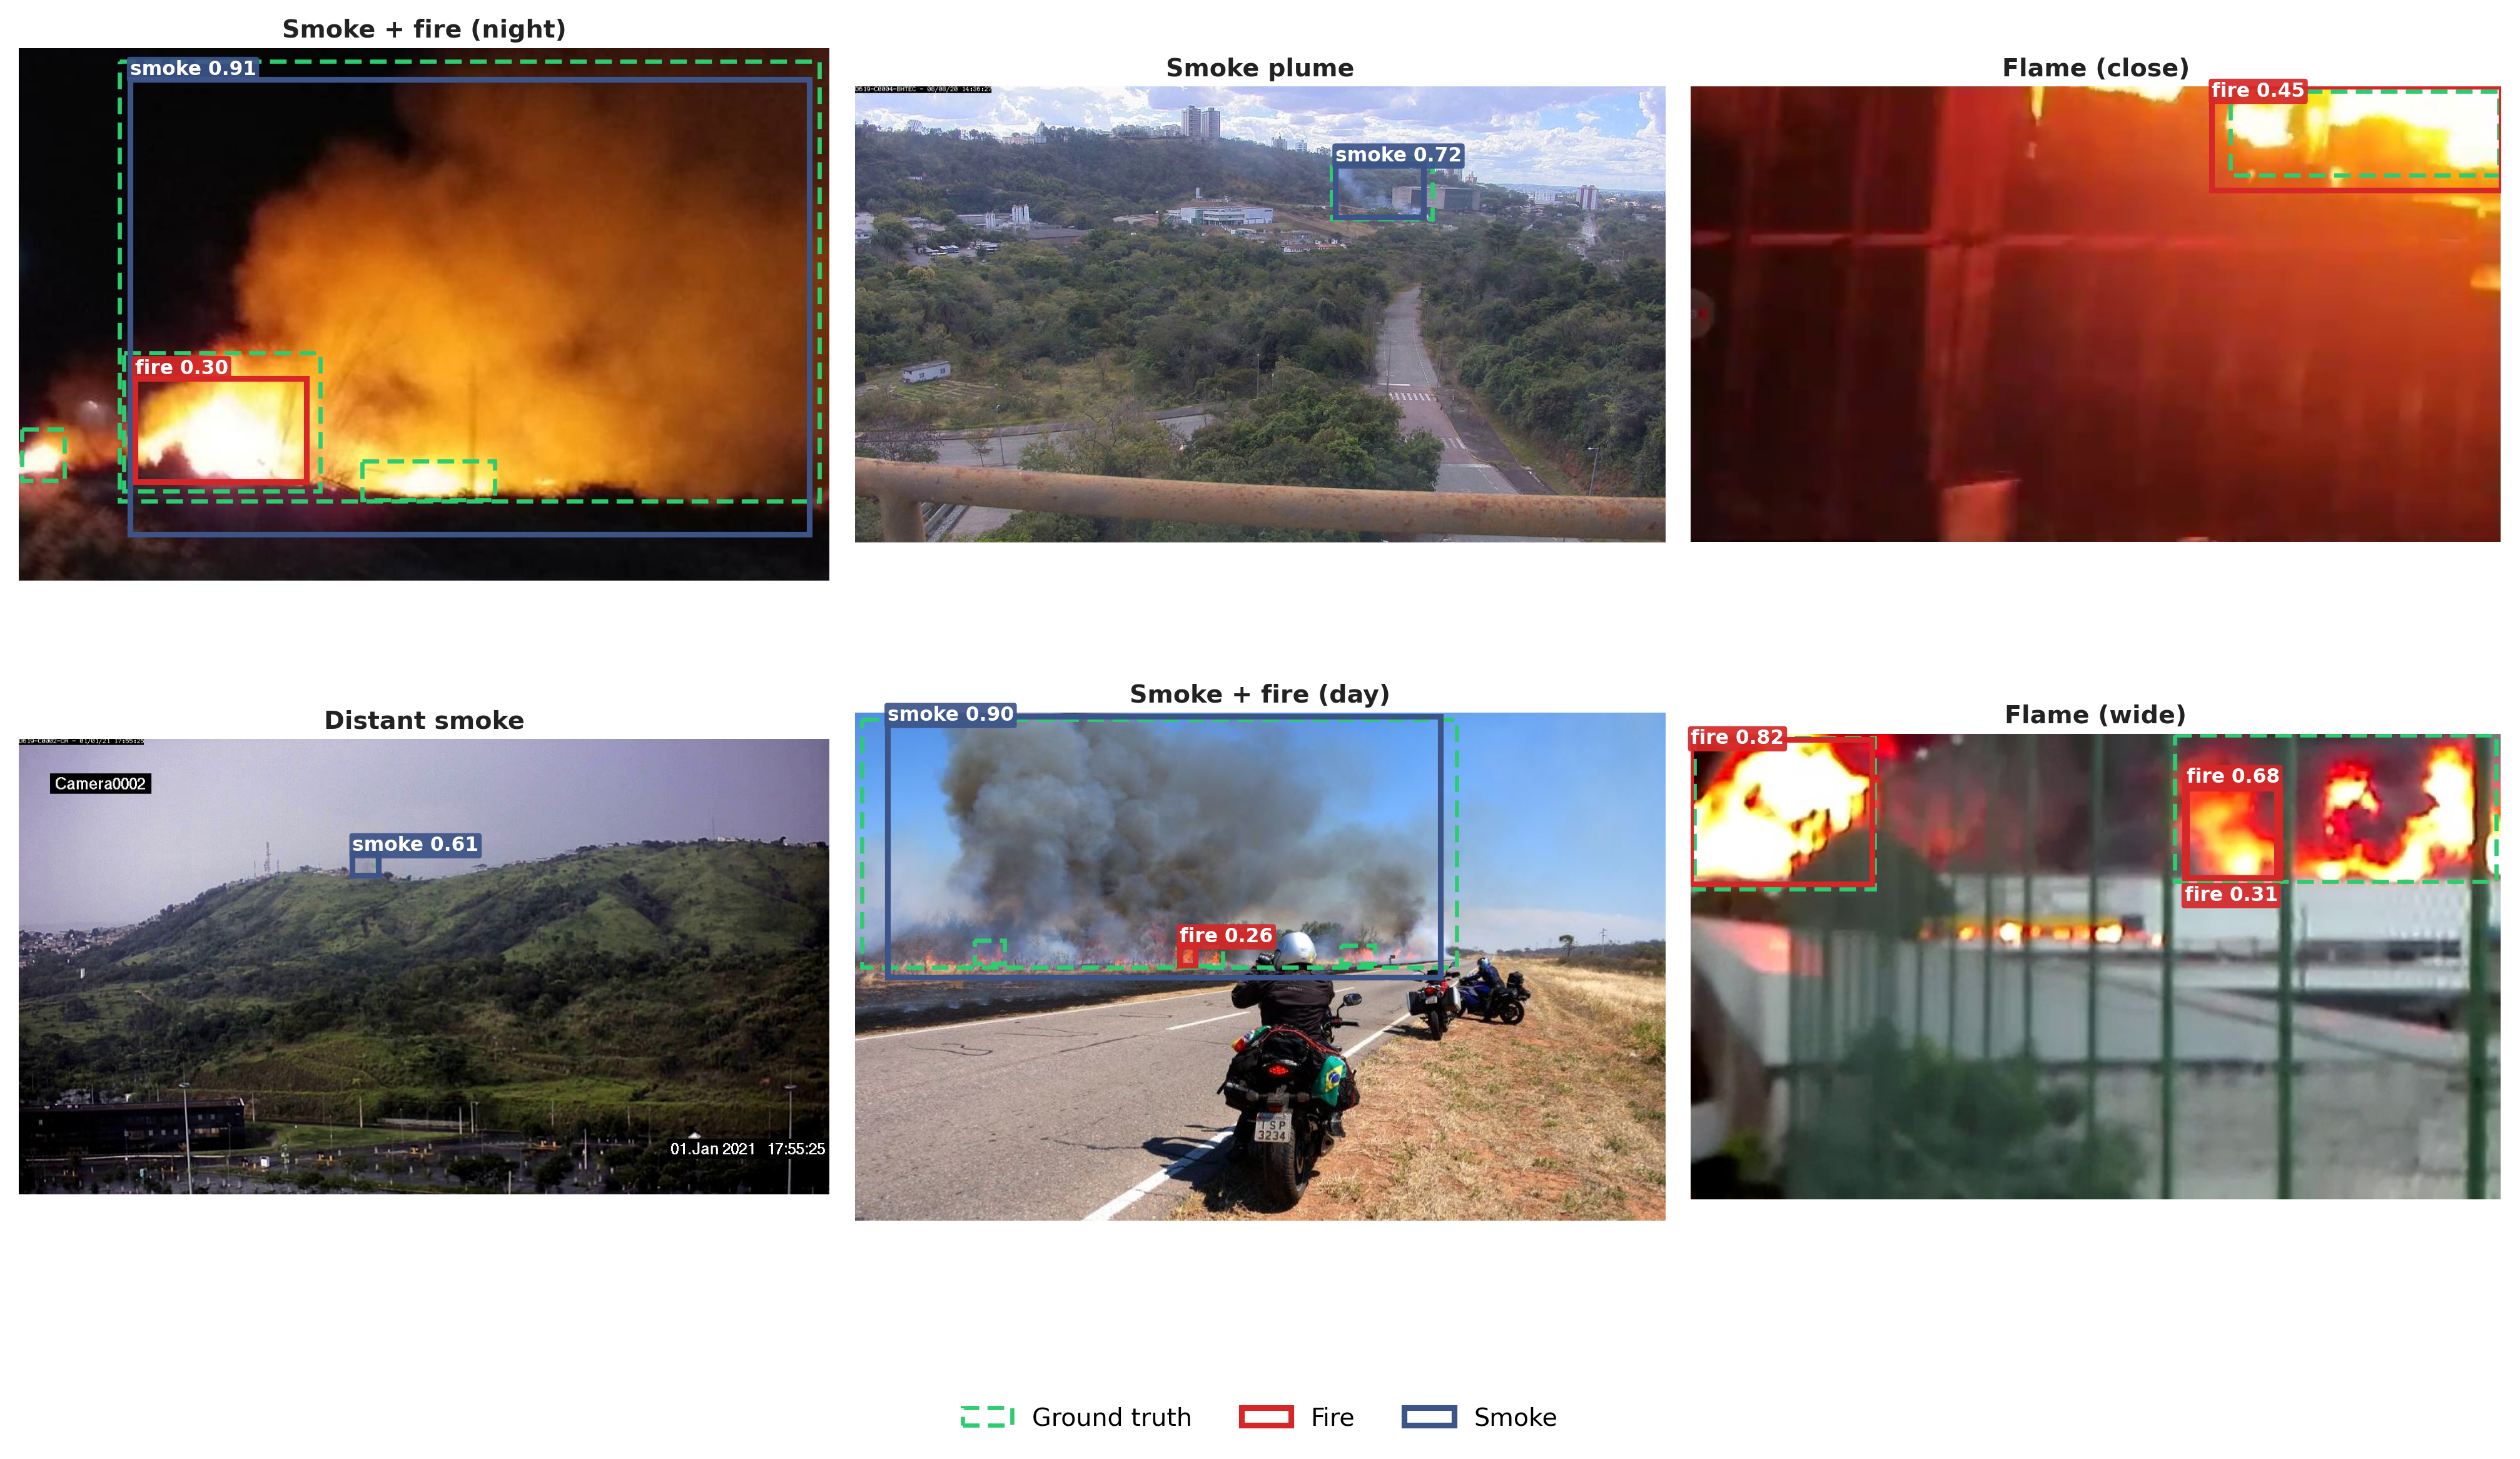
\includegraphics[width=0.8\textwidth]{fig_11_dfire_qualitative.png}
\caption[YOLO26s (CLAHE) detections on D-Fire]{YOLO26s (CLAHE) detections on six D-Fire test images. Dashed green: ground truth; solid: predictions with confidence. Low-confidence boxes are shown as-is.}
\label{fig:dfire_qualitative}
\end{figure*}

Figure~\ref{fig:performance_benchmark} places the two evaluation tracks side by side: the independently trained D-Fire detectors and the scene-classification recovery of the joint prototype.

\begin{figure*}[!t]
\centering
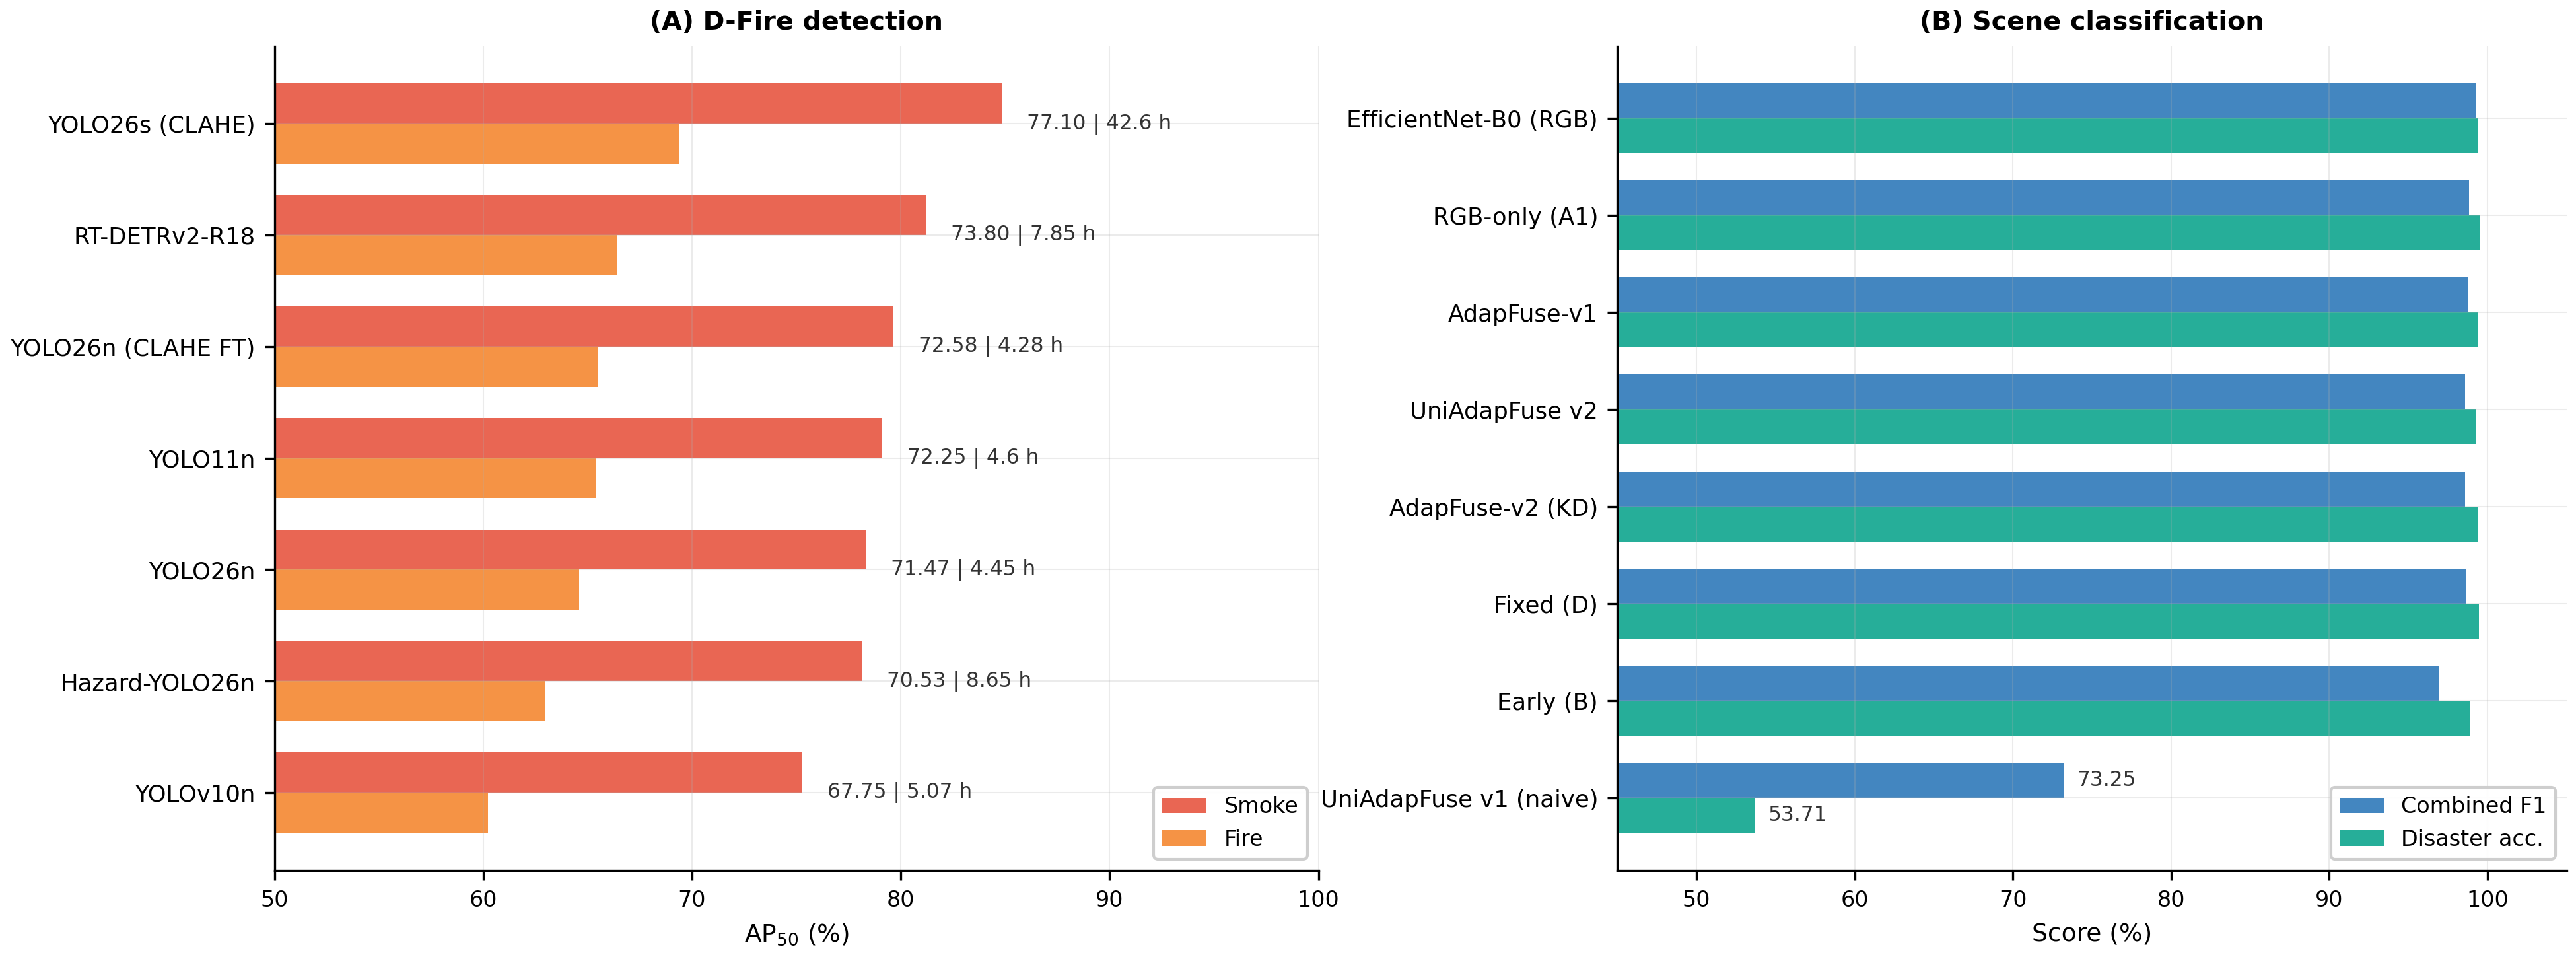
\includegraphics[width=0.8\textwidth]{fig_03_performance.png}
\caption[Detection and scene-classification results]{(A) D-Fire detectors: $\mathrm{mAP}_{50}$ and training time. (B) Scene classification: naive joint training (UniAdapFuse v1) falls to 53.71\% disaster accuracy; the v2 recipe restores 99.26\%, but its detection $\mathrm{mAP}_{50}$ is 0.0.}
\label{fig:performance_benchmark}
\end{figure*}

\subsection[Unified Perception Attempt: Classification Recovered, Detection Not]{Unified Perception Attempt: Negative Transfer Resolved for Classification but Not Detection}
\label{sec:uniadaptfuse}

\noindent\textbf{Summary of finding.} Naive joint training reaches only 53.71\% disaster accuracy, against 99.44\% for the classification-only model. A revised recipe (phased curriculum, stop-gradient isolation, distillation from AdapFuse-v1 and other changes) recovers classification to 98.57\% combined macro-F1, close to the standalone classifier (98.74\%), but the same saved checkpoint records a detection $\mathrm{mAP}_{50}$ of 0.0. The joint prototype therefore does not achieve joint perception, and all dense-detection results in this work (Section~\ref{sec:object_detection}) come from independently trained detectors on D-Fire, not from the unified architecture. The training logs point to numerical instability. The trainer silently skips any batch whose total loss is NaN or infinite. In the naive v1 run, 8 of the 17 logged epochs have a recorded training loss and accuracy of exactly zero, meaning every batch was skipped, and in the other epochs the logged training accuracy is computed over very few batches. In v2 only the final epoch (80) is logged, and there every training and validation batch was non-finite, as was the test loss. The collapse of v1 and the zero $\mathrm{mAP}_{50}$ of v2 are therefore at least partly explained by a joint loss that is not finite, not only by negative transfer. Other candidate causes include the small detection loss weight (0.2) or an error in the detection target or evaluation path; diagnosing them is left to future work.

While standalone object detectors provide spatial bounding boxes, they lack global disaster scene context and victim presence estimation. To bridge this gap, \textbf{UniAdapFuse} couples multi-scale visual-thermal Feature Pyramid Networks (FPN) with the tri-modal classification backbone, connected via Top-Down Context Gates (TDCG) and Bottom-Up Spatial Guidance (BUSG)~\cite{perez2018film}.

\subsubsection{Curriculum Warmup and Stop-Gradient Isolation}

Naive joint training of global scene classification and dense bounding box regression (UniAdapFuse v1) reaches only 53.71\% disaster accuracy, against 99.44\% for the classification-only AdapFuse-v1. Our working hypothesis was \textit{multi-task negative transfer}, in which dense regression losses (CIoU and objectness) disturb the shared visual backbone; as noted above, the log also shows widespread non-finite losses, so the collapse cannot be attributed to negative transfer alone.

UniAdapFuse v2 targets the classification side through three mechanisms: (1) \textit{Phased Curriculum Training}~\cite{bengio2009curriculum} with a 15-epoch classification-only warmup; (2) \textit{Stop-Gradient Isolation} (.detach()) applied to multi-scale pyramid feature maps before feeding the detection neck, so that detection gradients cannot backpropagate into the shared backbone; and (3) \textit{Differentiated Learning Rates} ($0.1\times$ backbone, $1.0\times$ classifier/bridge, $0.3\times$ detection head). The same run also distils from the trained AdapFuse-v1 checkpoint, lowers the base learning rate to $5\times10^{-4}$, trains for 80 instead of 50 epochs and reweights the losses. Because the distillation target is the standalone classifier that v2 is compared against, part of the recovery may simply be inherited from the teacher. Table~\ref{tab:uniadaptfuse_results} shows that classification is recovered while detection is not; which of the changes is responsible is not identified. Note that .detach() blocks detection gradients from reaching the shared backbone only; the detection neck and head still receive their own gradients, so the isolation mechanism by itself does not explain the zero $\mathrm{mAP}_{50}$.

\begin{table*}[!t]
\centering
\caption[UniAdapFuse scene-classification recovery]{UniAdapFuse scene-classification recovery ($n=10{,}951$). v2 recovers classification, but its detection $\mathrm{mAP}_{50}$ is 0.0.}
\label{tab:uniadaptfuse_results}
\resizebox{\textwidth}{!}{%
\begin{tabular}{@{}lccccccc@{}}
\toprule
\textbf{Model} & \textbf{Architecture / Training Mechanism} & \textbf{Dis.\ F1} & \textbf{Dis.\ Acc} & \textbf{Vic.\ F1} & \textbf{Vic.\ Acc} & \textbf{Comb.\ F1} & \textbf{Det. mAP$_{50}$} \\
\midrule
AdapFuse-v1 (standalone) & Classification only baseline & 0.9913 & 0.9944 & 0.9836 & 0.9884 & 0.9874 & n/a \\
UniAdapFuse v1 (naive) & Naive Joint End-to-End Training & 0.5669 & 0.5371 & 0.8980 & 0.9306 & 0.7325 & n/a \\
\textbf{UniAdapFuse v2 (enhanced)} & \textbf{Joint graph + isolation + KD} & \textbf{0.9920} & \textbf{0.9926} & \textbf{0.9794} & \textbf{0.9856} & \textbf{0.9857} & \textbf{0.0000} \\
\midrule
\multicolumn{2}{l}{\textit{v2 Classification Recovery Gain over v1}} & \textbf{+42.51 pp} & \textbf{+45.55 pp} & \textbf{+8.14 pp} & \textbf{+5.50 pp} & \textbf{+25.32 pp} & n/a \\
\bottomrule
\end{tabular}%
}
\end{table*}

UniAdapFuse v2 achieves \textbf{99.20\% disaster F1 and 98.57\% combined F1}, within 0.17 percentage points of the standalone classification reference, which is also its distillation teacher. This demonstrates recovery of the classification branch under the revised recipe, not the effect of gradient isolation alone. However, our uni\_adaptfuse\_v2\_test\_results.json reports $\mathrm{mAP}_{50}=0.0$ for detection. Our evidence therefore does not establish usable joint localization or compatibility between the tasks; the independent D-Fire detector results in Section~\ref{sec:object_detection} remain the valid localization benchmark.

\subsection{Multimodal Scene-Prior and Reliability Benchmark (Row-Level Split)}
\label{sec:classification_benchmark}

The global scene classification stream is intended to provide a prior for the detection stream. In the current evidence, scene classification and the independently trained D-Fire detectors are validated separately; a working scene-conditioned detector is not established. All twenty-six classification configurations were evaluated on the row-level held-out test set ($n=10{,}951$). Table~\ref{tab:main_results} presents the complete comparison ranked by Combined F1.

\textbf{Metric definition.} Throughout this chapter, \emph{Combined F1} is the unweighted mean of the two task-level macro-F1 scores,
\begin{equation}
    \text{Combined F1} = \tfrac{1}{2}\left(\text{macro-F1}_{\text{disaster}} + \text{macro-F1}_{\text{victim}}\right),
\end{equation}
where disaster macro-F1 averages over the four disaster classes and victim macro-F1 over the two victim-presence classes. Macro averaging weights every class equally, so rare classes are not hidden by the natural test distribution, and the outer mean weights the two tasks equally.

\textbf{Interpretation caveat.} Every score in Table~\ref{tab:main_results} comes from the row-level split, which is not grouped by capture sequence, and from a corpus in which source identity and label are entangled (Section~\ref{sec:per_source}). Differences between configurations are therefore within-collection comparisons, not evidence of generalization to new flights, sensors or regions.

\begin{table*}[!t]
\centering
\caption[All 26 multimodal classification models]{All 26 multimodal classification models, ranked by Combined F1 (row-level split, $n=10{,}951$). Under a capture-group-aware split, combined macro-F1 drops by 9.60\,pp (Section~\ref{sec:grouped_split}).}
\label{tab:main_results}
\resizebox{\textwidth}{!}{%
\begin{tabular}{@{}rllcccccc@{}}
\toprule
\textbf{Rank} & \textbf{Model / Experiment} & \textbf{Family / Type} & \textbf{Test Loss} & \textbf{Dis.\ F1} & \textbf{Vic.\ F1} & \textbf{Comb.\ F1} & \textbf{Dis.\ Acc} & \textbf{Vic.\ Acc} \\
\midrule
1 & \textbf{AdapFuse-v1 + EfficientNet-B0 (RGB)} & Visual Backbone & 0.0025 & 0.9923 & \textbf{0.9924} & \textbf{0.9924} & 0.9940 & \textbf{0.9947} \\
2 & \textbf{AdapFuse-v1 + MobileViT-XXS (RGB)} & Visual Backbone & 0.0103 & 0.9881 & 0.9916 & \textbf{0.9899} & 0.9931 & 0.9942 \\
3 & Baseline A1: RGB-Only & Unimodal Baseline & 0.0054 & 0.9924 & 0.9846 & 0.9885 & 0.9951 & 0.9891 \\
4 & AdapFuse-v1 + EfficientNet-B0 (Thermal) & Visual Backbone & 0.0095 & 0.9924 & 0.9837 & 0.9880 & 0.9950 & 0.9886 \\
5 & Ablation: No RUE (ablation\_no\_rue) & Component Ablation & 0.0094 & \textbf{0.9938} & 0.9812 & 0.9875 & \textbf{0.9957} & 0.9868 \\
6 & \textbf{AdapFuse-v1 (E): Base Teacher} & Proposed Method & \textbf{0.0020} & 0.9913 & 0.9836 & 0.9874 & 0.9944 & 0.9884 \\
7 & Ablation: No Nuisance Head & Component Ablation & 0.0092 & 0.9923 & 0.9821 & 0.9872 & 0.9942 & 0.9874 \\
8 & Intermediate Fixed Fusion (D) & Core Fusion Topology & 0.0059 & 0.9911 & 0.9828 & 0.9869 & 0.9947 & 0.9879 \\
9 & Late Fusion (C) & Core Fusion Topology & 0.0048 & 0.9916 & 0.9817 & 0.9867 & 0.9939 & 0.9871 \\
10 & AdapFuse-v1 + GDBlock & Audio Backbone & 0.0036 & 0.9888 & 0.9838 & 0.9863 & 0.9924 & 0.9886 \\
11 & AdapFuse-v2 KD Student (F) & Knowledge Distillation & 0.0035 & 0.9917 & 0.9805 & 0.9861 & 0.9944 & 0.9862 \\
12 & \textbf{UniAdapFuse v2 (Joint Cls + Det)} & Unified Multi-Task & n/a & 0.9920 & 0.9794 & \textbf{0.9857} & 0.9926 & 0.9856 \\
13 & RGB + Thermal Subset & Two-Sensor Subset & 0.0042 & 0.9870 & 0.9830 & 0.9850 & 0.9898 & 0.9880 \\
14 & RGB + Audio Subset & Two-Sensor Subset & 0.0021 & 0.9896 & 0.9802 & 0.9849 & 0.9942 & 0.9860 \\
15 & AdapFuse-v1 + Domain Prompts & Architecture Module & 0.0035 & 0.9885 & 0.9813 & 0.9849 & 0.9927 & 0.9869 \\
16 & AdapFuse-v2 KD + PANNS & Audio Backbone & 0.0041 & 0.9884 & 0.9813 & 0.9848 & 0.9924 & 0.9868 \\
17 & AdapFuse-v1 + Spatial Attention & Architecture Module & 0.0034 & 0.9874 & 0.9814 & 0.9844 & 0.9902 & 0.9869 \\
18 & Ablation: No Quality Tokens & Component Ablation & 0.0108 & 0.9881 & 0.9800 & 0.9840 & 0.9927 & 0.9858 \\
19 & Ablation: No Cross-Attention & Component Ablation & 0.0076 & 0.9894 & 0.9785 & 0.9839 & 0.9925 & 0.9848 \\
20 & AdapFuse-v1 + PANNS & Audio Backbone & 0.0038 & 0.9858 & 0.9792 & 0.9825 & 0.9907 & 0.9853 \\
21 & Ablation: No GRU Temporal Cell & Component Ablation & 0.0102 & 0.9863 & 0.9765 & 0.9814 & 0.9901 & 0.9833 \\
22 & Thermal + Audio Subset & Two-Sensor Subset & 0.0058 & 0.9880 & 0.9730 & 0.9805 & 0.9912 & 0.9809 \\
23 & Pseudo-thermal-only (A2) & Unimodal Baseline & 0.0102 & 0.9802 & 0.9684 & 0.9743 & 0.9838 & 0.9774 \\
24 & Early Fusion (B) & Core Fusion Topology & 0.0126 & 0.9832 & 0.9554 & 0.9693 & 0.9890 & 0.9685 \\
25 & UniAdapFuse v1 (Naive Joint) & Unified Multi-Task & 0.0137 & 0.5669 & 0.8980 & 0.7325 & 0.5371 & 0.9306 \\
26 & Audio-only (A3) & Unimodal Baseline & 0.1325 & 0.3820 & 0.4365 & 0.4093 & 0.7169 & 0.7746 \\
\bottomrule
\end{tabular}%
}
\end{table*}

\textbf{Fusion versus the RGB-only baseline.} Table~\ref{tab:main_results} does not show a fusion advantage on this split. The RGB-only baseline A1 (98.85\% combined F1) scores 0.11 points above AdapFuse-v1 (98.74\%), and the no-RUE ablation (98.75\%) matches the full model, so reliability-aware fusion does not raise row-level F1 above the RGB stream alone. AdapFuse-v1's advantage over A1 is limited to test loss (0.0020 against 0.0054). The two configurations ranked above A1 are AdapFuse-v1 with a stronger RGB backbone. Section~\ref{sec:unimodal_backbones} trains RGB-only models with the same backbones: RGB-only MobileViT-XXS (98.99\%) equals AdapFuse-v1 + MobileViT-XXS (98.99\%), and RGB-only EfficientNet-B0 (98.88\%) is 0.36 points below AdapFuse-v1 + EfficientNet-B0 (99.24\%), with the unimodal run limited to 12 epochs. These gaps are small single-seed differences. With the pseudo-thermal map derived from RGB and the audio label-matched, the fused inputs carry little information beyond the RGB frame, so a fusion benefit could only be tested with independent sensors.

\subsubsection{Unimodal Backbone Comparison}
\label{sec:unimodal_backbones}

To separate the effect of the backbone from the effect of fusion, each single-modality baseline was trained with three backbones: the original A1--A3 encoder and two alternatives. These models were trained through the same AdapFuse-UAV pipeline as the fused models, with the same classifier head, focal loss, balanced training subset, augmentation, mixed precision, early stopping and row-level test set ($n=10{,}951$) as Table~\ref{tab:main_results}. Every backbone was therefore trained inside the pipeline twice, once as a unimodal encoder and once as an AdapFuse-v1 encoder, so the two can be compared directly. Tables~\ref{tab:unimodal_rgb}--\ref{tab:unimodal_audio} report one table per modality. To bound training time, the new visual runs used a 12-epoch budget (2 warm-up epochs, cosine schedule, early-stopping patience 5); the original A1--A3 runs used a 50-epoch budget. The comparison therefore favours the original encoders, and every result is a single seed. Dense detection is evaluated on RGB only; those results are in Table~\ref{tab:dfire_results}.

\begin{table*}[!t]
\centering
\caption[RGB-only scene classification]{RGB-only scene classification with three backbones ($n=10{,}951$). Epochs: run / budget. Best in bold.}
\label{tab:unimodal_rgb}
\resizebox{\textwidth}{!}{%
\begin{tabular}{@{}llcccccccc@{}}
\toprule
\textbf{Model} & \textbf{Backbone} & \textbf{Params} & \textbf{Epochs} & \textbf{Test Loss} & \textbf{Dis.\ F1} & \textbf{Vic.\ F1} & \textbf{Comb.\ F1} & \textbf{Dis.\ Acc} & \textbf{Vic.\ Acc} \\
\midrule
A1 & MobileNetV3-Small & 1.22M & 50 / 50 & \textbf{0.0054} & \textbf{0.9924} & 0.9846 & 0.9885 & \textbf{0.9951} & 0.9891 \\
A1b & EfficientNet-B0 & 4.66M & 12 / 12 & 0.0125 & 0.9887 & 0.9889 & 0.9888 & 0.9923 & 0.9922 \\
A1c & MobileViT-XXS & \textbf{1.12M} & 12 / 12 & 0.0105 & 0.9882 & \textbf{0.9915} & \textbf{0.9899} & 0.9921 & \textbf{0.9941} \\
\bottomrule
\end{tabular}%
}
\end{table*}

\begin{table*}[!t]
\centering
\caption[Pseudo-thermal-only scene classification]{Pseudo-thermal-only scene classification (1-channel, derived from RGB). A2 stopped early at epoch 36 of 50.}
\label{tab:unimodal_thermal}
\resizebox{\textwidth}{!}{%
\begin{tabular}{@{}llcccccccc@{}}
\toprule
\textbf{Model} & \textbf{Backbone} & \textbf{Params} & \textbf{Epochs} & \textbf{Test Loss} & \textbf{Dis.\ F1} & \textbf{Vic.\ F1} & \textbf{Comb.\ F1} & \textbf{Dis.\ Acc} & \textbf{Vic.\ Acc} \\
\midrule
A2 & ResNet-18 (1-ch) & 11.43M & 36 / 50 & \textbf{0.0102} & 0.9802 & 0.9684 & 0.9743 & 0.9838 & 0.9774 \\
A2b & EfficientNet-B0 (1-ch) & 4.66M & 12 / 12 & 0.0126 & \textbf{0.9927} & \textbf{0.9794} & \textbf{0.9860} & \textbf{0.9934} & \textbf{0.9855} \\
A2c & MobileViT-XXS (1-ch) & \textbf{1.12M} & 12 / 12 & 0.0117 & 0.9905 & 0.9788 & 0.9846 & 0.9918 & 0.9851 \\
\bottomrule
\end{tabular}%
}
\end{table*}

\begin{table*}[!t]
\centering
\caption[Audio-only scene classification]{Audio-only scene classification (label-matched ESC-50 log-mel; 47.2\% of test rows have no audio). A3b and A3c stopped early with identical, degenerate results.}
\label{tab:unimodal_audio}
\resizebox{\textwidth}{!}{%
\begin{tabular}{@{}llcccccccc@{}}
\toprule
\textbf{Model} & \textbf{Backbone} & \textbf{Params} & \textbf{Epochs} & \textbf{Test Loss} & \textbf{Dis.\ F1} & \textbf{Vic.\ F1} & \textbf{Comb.\ F1} & \textbf{Dis.\ Acc} & \textbf{Vic.\ Acc} \\
\midrule
A3 & AudioCNN (scratch) & 0.11M & 50 / 50 & \textbf{0.1325} & 0.3820 & 0.4365 & 0.4093 & \textbf{0.7169} & \textbf{0.7746} \\
A3b & CNN6-style$^\dagger$ & 1.62M & 24 / 40 & 0.2610 & 0.4153 & 0.5777 & 0.4965 & 0.5673 & 0.6163 \\
A3c & AudioCNN + GDBlock & \textbf{0.07M} & 25 / 40 & 0.2625 & 0.4153 & 0.5777 & 0.4965 & 0.5673 & 0.6163 \\
\bottomrule
\multicolumn{10}{@{}l}{\footnotesize $^\dagger$Only 8 of the encoder's 20 weight tensors (batch-normalisation parameters) load from the PANNs AudioSet checkpoint; no convolution weights load, so the encoder is effectively trained from scratch.}
\end{tabular}%
}
\end{table*}

\textbf{RGB.} The three RGB backbones fall within 0.14 combined-F1 points of each other (98.85--98.99\%). MobileViT-XXS gives the best combined F1 and victim-presence F1 with the fewest parameters, while MobileNetV3-Small keeps the best disaster F1 and test loss after a four-times longer training budget. RGB-only classification is at its ceiling on this split, so a stronger RGB encoder adds little.

\textbf{Pseudo-thermal.} Changing the backbone matters more here: EfficientNet-B0 raises combined F1 from 97.43\% (ResNet-18) to 98.60\% in 12 epochs, and MobileViT-XXS reaches 98.46\% with one-tenth of ResNet-18's parameters. MobileViT-XXS validation F1 was still rising at epoch 12 (97.28\% at epoch 11), so its score is limited by the training budget. The best pseudo-thermal model remains 0.39 points below the best RGB model, which is expected because the map is computed from the same RGB frame and discards colour.

\textbf{Audio.} The audio scores are shaped by the data construction rather than by acoustic recognition. Three facts explain A3. First, 47.2\% of test rows have no audio and receive an all-zero input. Second, no collapse/flood or other-hazard row has audio, so those two classes cannot be recognised from sound, which caps disaster macro-F1. Third, on rows that do have audio, the clip's ESC-50 class encodes the label: fire/smoke rows always receive a ``crackling fire'' clip and clean rows never do (Section~\ref{sec:dataset_sources}). A3's disaster accuracy (71.69\%) matches what a model would score if it were correct on essentially every row with audio and predicted fire/smoke on every silent row (7{,}855 of 10{,}951 rows, 71.73\%), and its victim accuracy (77.46\%) equals the share of no-person rows, so it predicts ``no person'' throughout. The low 38.2\% disaster macro-F1 of A3 therefore does not show that the audio is uninformative; it shows missing inputs, absent classes, and a label shortcut. The two alternative encoders did not even learn that shortcut. The CNN6-style encoder (which loaded no pretrained convolution weights) and GDBlock produced exactly the same test metrics to every reported digit, their training accuracy plateaued at 55.7\% from the first epochs, and their training loss hardly changed, which indicates a shared degenerate decision rule. Their higher combined F1 than A3 (49.65\% against 40.93\%) is therefore not an improvement: A3 has higher accuracy on both tasks and a lower test loss. None of these results measures UAV acoustic sensing.

\begin{table*}[!t]
\centering
\caption[Accuracy vs.\ cost of visual backbones]{Combined F1 (\%) vs.\ cost of the visual backbones (cost from Table~\ref{tab:backbone_candidates}). Fused: AdapFuse-v1 with that backbone. $^\dagger$Lower bound. -- = not trained.}
\label{tab:backbone_accuracy_cost}
\resizebox{\textwidth}{!}{%
\begin{tabular}{@{}lcccccc@{}}
\toprule
\textbf{Backbone} & \textbf{GMACs} & \textbf{Params (M)} & \textbf{RGB-only} & \textbf{Pseudo-thermal-only} & \textbf{Fused (RGB stream)} & \textbf{Fused (thermal stream)} \\
\midrule
MobileNetV3-Small & \textbf{0.06} & 0.93 & 98.85 & -- & 98.74 & -- \\
MobileViT-XXS & 0.30$^\dagger$ & 0.95 & \textbf{98.99} & 98.46 & 98.99 & -- \\
EfficientNet-B0 & 0.39 & 4.01 & 98.88 & \textbf{98.60} & \textbf{99.24} & \textbf{98.80} \\
ResNet-18 & 1.81 & 11.18 & -- & 97.43 & -- & 98.74 \\
\bottomrule
\end{tabular}%
}
\end{table*}

Table~\ref{tab:backbone_accuracy_cost} gives the outcome of the selection in Section~\ref{sec:backbone_selection}. For RGB, the lowest-cost encoder is within 0.14 points of the best, so MobileNetV3-Small remains a reasonable default at one-fifth of MobileViT-XXS's MACs. For pseudo-thermal, the over-budget ResNet-18 is both the most expensive and the least accurate choice; EfficientNet-B0 is 1.17 points better at 21\% of its MACs, which makes it the better default for that stream.

\textbf{Matched-backbone fusion comparison.} With the backbone held fixed, fusion adds 0.36 combined-F1 points for EfficientNet-B0 on RGB (99.24\% against 98.88\%), nothing for MobileViT-XXS on RGB (98.99\% for both), and 0.20 points for EfficientNet-B0 on the pseudo-thermal stream (98.80\% against 98.60\%). The unimodal runs had a shorter budget (12 epochs, against 50-epoch budgets for the three fused models, whose best checkpoints came at epochs 39, 36 and 48), so these small gaps do not show that fusion helps; they are consistent with the conclusion above that the fused inputs add little beyond the RGB frame.

\subsubsection{Comparison with Published Results on Public Benchmarks}
\label{sec:public_benchmark_results}

The row-level scores above cannot be compared with published work, because our corpus merges six sources and splits them at random. To obtain comparable numbers, three models were retrained through the same AdapFuse-UAV pipeline under the published protocols of two public datasets (Section~\ref{sec:public_benchmarks_related}): RGB-only MobileNetV3-Small (A1), RGB-only EfficientNet-B0 (A1b) and AdapFuse-v1 with RGB and its derived pseudo-thermal map (audio absent). All used ImageNet-pretrained encoders, focal loss, the same augmentation (no synthetic corruption), and model selection on the validation split; each is a single seed.

\textbf{AIDER protocol.} The 6{,}433-image AIDER subset was split per class with exactly the train/validation/test counts of Lee et al.~\cite{lee2023wattefnet} (3{,}207 / 753 / 2{,}473; five classes, 71\% of test images normal). Lee et al.\ describe this split as 4:1:2, although the listed counts are closer to 5:1:4; we follow the counts. Unlike Lee et al., who under-sample the training and validation sets, our models trained for up to 30 epochs without resampling.

\begin{table*}[!t]
\centering
\caption[AIDER results]{AIDER results. (a) 4:1:2 protocol of Lee et al.~\cite{lee2023wattefnet} (2{,}473 test images), which we follow. (b) Earlier protocol with a different test set, for reference only. Our F1 is macro-averaged (weighted F1 in brackets).}
\label{tab:public_aider}
\resizebox{\textwidth}{!}{%
\begin{tabular}{@{}llccc@{}}
\toprule
\textbf{Model} & \textbf{Source} & \textbf{Params (M)} & \textbf{F1 (\%)} & \textbf{Accuracy (\%)} \\
\midrule
\multicolumn{5}{@{}l}{\textit{(a) 4:1:2 protocol of Lee et al., 2{,}473 test images}} \\
EfficientNet & Lee et al.~\cite{lee2023wattefnet} & 3.50 & 80.0 & -- \\
MobileNetV2 & Lee et al.~\cite{lee2023wattefnet} & 2.28 & 81.0 & -- \\
EmergencyNet~\cite{kyrkou2020emergencynet} & Lee et al.~\cite{lee2023wattefnet} & 0.09 & 83.1 & -- \\
WATT-EffNet-3-6 & Lee et al.~\cite{lee2023wattefnet} & 0.69 & 88.5 & -- \\
RGB-only MobileNetV3-Small (A1) & Ours & 1.22 & 93.02 [96.48] & 96.48 \\
RGB-only EfficientNet-B0 (A1b) & Ours & 4.67 & \textbf{94.00} [\textbf{97.00}] & \textbf{97.01} \\
AdapFuse-v1 (RGB + pseudo-thermal) & Ours & 12.94 & 91.86 [95.79] & 95.79 \\
\midrule
\multicolumn{5}{@{}l}{\textit{(b) Protocol of Kyrkou and Theocharides, 2{,}123 test images, weighted F1 (not comparable with (a))}} \\
EmergencyNet & Kyrkou and Theocharides~\cite{kyrkou2020emergencynet}$^\ddagger$ & 0.09 & 93.6 & -- \\
TinyEmergencyNet & Mogaka et al.~\cite{mogaka2024tinyemergencynet}$^\ddagger$ & 0.04 & 89.5 & -- \\
TakuNet (FP32) & Rossi et al.~\cite{rossi2025takunet} & 0.04 & 93.8 & -- \\
GlimmerNet & Nedeljkovi{\'c}~\cite{nedeljkovic2025glimmernet} & 0.03 & 94.2 & -- \\
\bottomrule
\multicolumn{5}{@{}l}{\footnotesize $^\ddagger$F1 as reported in the comparison tables of Rossi et al.~\cite{rossi2025takunet} and Nedeljkovi{\'c}~\cite{nedeljkovic2025glimmernet}.}
\end{tabular}%
}
\end{table*}

All three of our models exceed the published F1 scores under the protocol we follow (Table~\ref{tab:public_aider}a), with RGB-only EfficientNet-B0 at 94.00\% macro-F1 against 88.5\% for WATT-EffNet. The comparison is not like-for-like: our encoders start from ImageNet weights, whereas Lee et al.\ trained from scratch to study lightweight design, and the F1 averaging of the published table is not stated. The margin is therefore evidence that ImageNet transfer inside our pipeline is effective on AIDER, not that our architectures are better designed. More recent lightweight networks (Table~\ref{tab:public_aider}b) reach 93.6--94.2\% weighted F1 with 0.03--0.09\,M parameters, but on a different split; our weighted F1 of 97.00\% is higher, yet because the test images differ and those networks are 50--150$\times$ smaller (TakuNet, for example, is trained from scratch~\cite{rossi2025takunet}), we do not claim to outperform them. Fusion again does not help: AdapFuse-v1 is 2.14 points below RGB-only EfficientNet-B0, because the pseudo-thermal map carries no information beyond the RGB frame.

\begin{table*}[!t]
\centering
\caption[Per-class AIDER results]{Per-class results on the AIDER 4:1:2 test set (P, R, F1 in \%; $n$: test images).}
\label{tab:public_aider_perclass}
\resizebox{\textwidth}{!}{%
\begin{tabular}{@{}lrccccc@{}}
\toprule
 & & \multicolumn{3}{c}{\textbf{RGB-only EfficientNet-B0}} & \textbf{RGB-only MobileNetV3-S} & \textbf{AdapFuse-v1} \\
\cmidrule(lr){3-5}
\textbf{Class} & \textbf{$n$} & \textbf{P} & \textbf{R} & \textbf{F1} & \textbf{F1} & \textbf{F1} \\
\midrule
Normal & 1{,}756 & 98.24 & 98.52 & \textbf{98.38} & 98.06 & 97.67 \\
Fire & 209 & 97.14 & 97.61 & 97.37 & \textbf{97.39} & 94.69 \\
Collapsed building & 103 & 86.24 & 91.26 & \textbf{88.68} & 86.64 & 85.98 \\
Flood & 211 & 96.21 & 96.21 & \textbf{96.21} & 95.13 & 95.26 \\
Traffic incident & 194 & 92.31 & 86.60 & \textbf{89.36} & 87.87 & 85.71 \\
\midrule
Macro average & 2{,}473 & -- & -- & \textbf{94.00} & 93.02 & 91.86 \\
\bottomrule
\end{tabular}%
}
\end{table*}

Table~\ref{tab:public_aider_perclass} shows where the errors lie. Normal, fire and flood scenes are recognised with at least 95\% F1 by all three models, while collapsed buildings (86.0--88.7\%) and traffic incidents (85.7--89.4\%) remain the weakest classes; for traffic, recall (86.6\%) is the limiting factor, meaning that accident scenes are mostly lost to the normal class. Lee et al.\ do not tabulate per-class F1, but their confusion matrix identifies traffic incidents as their best class and normal scenes as their worst~\cite{lee2023wattefnet}, the reverse of our pattern, which is consistent with our models having seen far more normal than incident images during training (no resampling).

\textbf{FLAME protocol.} Models trained on the official FLAME training folder (39{,}375 frames from a Matrice 200 with a Zenmuse X4S), with a random 20\% of it held out for validation as in the original paper, and were tested on the official test folder (8{,}617 frames from a Phantom 3)~\cite{shamsoshoara2021aerial}. Training was limited to 10 epochs.

\begin{table*}[!t]
\centering
\caption[FLAME fire/no-fire classification]{FLAME fire/no-fire results, official protocol (8{,}617 test frames from a different drone than training). Fire recall: sensitivity; no-fire recall: specificity. Zhang/Wang (2022) as reported by Deng et al.~\cite{deng2025lightweight}. -- = not reported.}
\label{tab:public_flame}
\resizebox{\textwidth}{!}{%
\begin{tabular}{@{}llcccccc@{}}
\toprule
\textbf{Model} & \textbf{Source} & \textbf{Best ep.} & \textbf{Val.\ F1} & \textbf{Test Acc.} & \textbf{Test F1} & \textbf{Fire rec.} & \textbf{No-fire rec.} \\
\midrule
Xception & Shamsoshoara et al.\ (2021)~\cite{shamsoshoara2021aerial} & -- & -- & 76.23 & -- & -- & -- \\
ResNet-50 & Zhang/Wang (2022)~\cite{deng2025lightweight} & -- & -- & 79.48 & -- & -- & -- \\
EfficientNet-B5 + DenseNet-201 & Ghali et al.\ (2022)~\cite{ghali2022uavwildfire} & -- & -- & 85.12 & 84.77 & -- & -- \\
MV2-CBAM (mean of 30 runs) & Deng et al.\ (2025)~\cite{deng2025lightweight} & -- & -- & 85.82 & -- & -- & -- \\
MV2-CBAM (5-model ensemble) & Deng et al.\ (2025)~\cite{deng2025lightweight} & -- & -- & \textbf{88.05} & -- & -- & -- \\
FireXplainNet & Khan and Park (2024)~\cite{khan2024firexplainnet} & -- & -- & 87.32 & \textbf{86.50} & 88.87 & \textbf{88.01} \\
\midrule
RGB-only MobileNetV3-Small & Ours & 1 & 99.86 & 69.41 & 62.76 & \textbf{93.65} & 33.62 \\
RGB-only EfficientNet-B0 & Ours & 1 & 99.92 & 83.72 & 82.85 & 89.10 & 75.80 \\
AdapFuse-v1 (RGB + pseudo-th.) & Ours & 9 & 99.96 & 75.53 & 72.93 & 89.33 & 55.14 \\
\bottomrule
\end{tabular}%
}
\end{table*}

Table~\ref{tab:public_flame} shows the effect this thesis has to contend with. Every model scores 99.86--99.96\% F1 on validation frames from the training drone and 62.76--82.85\% on the test drone, a drop of 17 to 37 points. RGB-only EfficientNet-B0 reaches 83.72\% test accuracy. That is above the original Xception baseline (76.23\%) and the ResNet-50 result (79.48\%), but 1.40 to 4.33 points below three later methods: the ensemble of Ghali et al.\ (85.12\%), MV2-CBAM (85.82\% averaged over 30 runs, 88.05\% as a five-model ensemble) and FireXplainNet (87.32\%). MobileNetV3-Small (69.41\%) and AdapFuse-v1 (75.53\%) fall below even the Xception baseline. The per-class columns locate the shortfall. Our models find fire as reliably as the best published model (89.1--93.7\% fire recall against 88.9\% for FireXplainNet), but they reject far fewer clean frames (33.6--75.8\% no-fire recall against 88.0\%): on the new camera they call many fire-free scenes fire. The bias is strongest in the weaker models. This is consistent with the camera change pushing predictions towards fire, the majority class in training (64\% of frames), while the fire cue itself still transfers. Because the in-domain validation split is saturated from the first epoch, it cannot guide model selection for the new camera: both RGB-only runs kept their epoch-1 checkpoints and stopped early. These results support the conclusion of Section~\ref{sec:grouped_split}: scores on frames from the same capture as training are near ceiling and overstate performance on new hardware. They also show that on a genuine cross-camera test the stronger backbone matters more than fusion with an RGB-derived map.

\subsubsection{Row-Level False Positives and Probabilistic Calibration}
\label{sec:adaptfuse_extended}

Table~\ref{tab:adaptfuse_extended} reports extended metrics for AdapFuse-v1, including our averages of the \textit{Reliability and Uncertainty Estimator (RUE)} gates. Because the nuisance branch is unsupervised and the gates are not trained against degradation targets, these values describe the fitted model; they do not measure the effect of either component.

\begin{table*}[!t]
\centering
\caption[AdapFuse-v1 extended evaluation metrics]{AdapFuse-v1 extended evaluation metrics ($n=10{,}951$)}
\label{tab:adaptfuse_extended}
\begin{tabular}{@{}ll>{\raggedright\arraybackslash}p{5.2cm}@{}}
\toprule
\textbf{Metric} & \textbf{Value} & \textbf{Operational Significance} \\
\midrule
Disaster F1 (macro)    & 0.9913 & 4-class multi-disaster categorization \\
Disaster Accuracy      & 0.9944 & Evaluated on natural distribution \\
Disaster Precision     & 0.9870 & High confidence in positive alerts \\
Disaster Recall        & 0.9957 & Extremely low miss rate on active hazards \\
Victim F1 (macro)      & 0.9836 & Binary survivor presence detection \\
Victim Accuracy        & 0.9884 & \\
\midrule
\textbf{False Positive Rate (FPR)} & \textbf{0.0073} & Row-level scene-classification FPR \\
\textbf{Expected Calibration Error (ECE)} & \textbf{0.0337} & Calibration statistic on the row-level split \\
\textbf{Test Loss (Focal)} & \textbf{0.0020} & Lowest across all evaluated architectures \\
\midrule
Avg Reliability: RGB$^\dagger$   & 0.972  & $\approx$1.0 on every row with RGB; unchanged under corruption \\
Avg Reliability: Pseudo-thermal$^\dagger$ & 0.972 & $\approx$1.0 on every row with the map; unchanged under corruption \\
Avg Reliability: Audio$^\dagger$ & \textbf{0.006}  & $\approx$0.011 on rows with audio; label-matched audio largely ignored \\
\midrule
Total Parameters       & 12.94M & Compact multi-branch footprint \\
Inference Latency (batch=1) & 14.32 ms & 69.9 FPS on workstation RTX 5090 \\
\bottomrule
\end{tabular}

\vspace{1mm}
\parbox{0.95\textwidth}{\footnotesize $^\dagger$Means over all 10{,}951 test rows. The model sets a gate to zero whenever its modality is missing, and the averaging script (reliability\_analysis.py) includes those rows. 0.972 equals the fraction of test rows that have RGB and pseudo-thermal inputs (10{,}646/10{,}951 = 0.9721), so both image gates sit at $\approx$1.0 on every row that has the input. The audio mean of 0.006 over all rows corresponds to $\approx$0.011 over the 5{,}781 rows that have an audio clip.}
\end{table*}

\textbf{Observed row-level false-positive rate (0.73\%):}
Our evaluation reports a 0.73\% false-positive rate for scene classification on the row-level test split. This is not an operational field false-alarm study and cannot be causally attributed to the NuisanceAwareHead, because our trainer passes nuisance\_gt=None and its nuisance loss is zero.

\textbf{Learned modality gates:}
The reported averages (audio 0.006, image streams 0.972) include rows whose gate is forced to zero because the modality is missing. Restricted to rows that have each input, the row-level model's RGB and pseudo-thermal gates are saturated at $\approx$1.0 and its audio gate is $\approx$0.011; the RUE is therefore effectively passing both image streams through unchanged and switching audio off. In this run the learned representation largely ignores the label-matched ESC-50 channel. The audio carries no information about the specific scene, but it does carry the fire/clean label on rows that have it (Section~\ref{sec:dataset_sources}), so ignoring it is only one of two solutions the data allow; with RGB already near ceiling on this split, the model had little to gain from the shortcut. The low audio gate is therefore a consequence of the data construction and of this training run, not evidence of learned reliability estimation. It is also not a stable property of the architecture: the grouped-split retraining (Section~\ref{sec:grouped_gates}) converges to the opposite audio gate. Likewise, the RGB and pseudo-thermal gates remain essentially constant across all tested corruption severities (Section~\ref{sec:robustness_stress_test}). In our model, the RUE behaves as a learned, largely input-independent feature weighting rather than as a dynamic reliability estimator; corruption-sensitive gating would require training with explicit degradation targets and evaluating gate response against measured degradation, neither of which is present here.

\subsubsection{Per-Module Latency Breakdown}

Table~\ref{tab:latency_profile} breaks down the 14.32\,ms total inference latency of AdapFuse-v1 by module, measured at batch size 1 on an NVIDIA RTX 5090 (32\,GB VRAM) (establishing the computational efficiency baseline prior to physical embedded edge deployment in future work).

\begin{table*}[!t]
\centering
\caption[Per-module inference latency of AdapFuse-v1]{Per-module inference latency of AdapFuse-v1 (batch 1, workstation GPU)}
\label{tab:latency_profile}
\resizebox{\textwidth}{!}{%
\begin{tabular}{@{}lrr@{}}
\toprule
\textbf{Module} & \textbf{Latency (ms)} & \textbf{\% of Total Pipeline} \\
\midrule
RGB Backbone (MobileNetV3-Small) & 6.37 & 44.5\% \\
Pseudo-Thermal Backbone (ResNet-18)& 5.17 & 36.1\% \\
Audio Backbone (AudioCNN)        & 0.47 &  3.3\% \\
Feature Projectors (3 streams)   & 0.30 &  2.1\% \\
Quality Token Heads              & 0.32 &  2.2\% \\
\textbf{Reliability and Uncertainty Estimator (RUE)} & \textbf{0.85} & \textbf{5.9\%} \\
Cross-Modal Attention Layer      & 0.22 &  1.5\% \\
Single-step GRU Cell             & 0.19 &  1.3\% \\
NuisanceAwareHead                & 0.37 &  2.6\% \\
Unattributed (end-to-end minus module sum) & 0.07 & 0.5\% \\
\midrule
\textbf{Total Inference Pipeline (end-to-end)} & \textbf{14.32} & \textbf{100.0\%} \\
\bottomrule
\end{tabular}%
}
\end{table*}

The feature extractors (RGB, pseudo-thermal, and audio backbones) account for 83.8\% of the measured execution time. The RUE, attention, GRU, and nuisance branch together add 1.63\,ms, with gate computation requiring 0.85\,ms (5.9\%). At batch size 1 on a large GPU, latency is dominated by the number of sequential kernel launches rather than by arithmetic, which is why MobileNetV3-Small (0.06\,GMACs, many small layers) takes longer than ResNet-18 (1.81\,GMACs) and why a small MLP such as the RUE costs 0.85\,ms; these timings therefore do not transfer to an embedded accelerator. A separate end-to-end measurement in our evaluation script gave 12.10\,ms, so run-to-run variation is of the order of 2\,ms. This profiles implementation overhead on the workstation GPU; it does not establish that the learned gates respond dynamically to degradation.

\textbf{Measurement scope.} All latency figures in this section were measured on an NVIDIA RTX 5090 workstation GPU (32\,GB VRAM), whose power draw far exceeds the $\leq$15\,W embedded payload targeted in Section~\ref{sec:tech_requirements}. They are not estimates of on-board UAV latency or power. Latency, power and thermal behaviour on an embedded accelerator, with and without INT8 quantisation, have not been measured and remain future work.

\subsection{Leakage-Resistant Grouped-Split Evaluation}
\label{sec:grouped_split}

Every result reported so far uses the row-level stratified split described in Section~\ref{sec:dataset_split}, which does not group by source video, flight, or near-duplicate sequence. To quantify how much of the near-ceiling performance depends on that choice, a capture-group-aware split was rebuilt and AdapFuse-v1 was retrained on it from scratch.

\textbf{Grouped split construction.} The 72{,}997 rows were repartitioned into 50{,}845 training, 11{,}055 validation, and 11{,}097 test rows under a capture-group constraint, yielding 9{,}267 / 2{,}003 / 2{,}002 disjoint capture groups. FLAME does not expose true video or flight identifiers in its released files, so its frames are blocked in contiguous runs of 250 as an explicit adjacent-frame proxy; C2A augmentations and SARD Roboflow variants are grouped by original-image identity; ESC-50 folds 1--3, 4 and 5 are assigned to train, validation and test respectively, and visual rows are re-paired only with clips from their own partition. The generated split contains zero capture-group overlap and zero ESC-50 path overlap across the three partitions.

\textbf{Training recipe differences.} The grouped retraining was not a like-for-like repeat of the row-level run. Our run configuration (resolved\_config.yaml) shows that it was trained with batch size 2 instead of 16, and with class balancing disabled (use\_balanced: false), i.e.\ on the 50{,}845 unbalanced grouped training rows (46.7\% fire/smoke, 4.0\% other hazard) rather than on a Stratified Balanced Subset. Optimiser, learning-rate schedule, epochs, early stopping and missing-modality dropout were unchanged. Consequently, the difference between the two columns of Table~\ref{tab:grouped_comparison} combines three effects (the split, the class balance of the training data, and the batch size), and the present runs cannot separate them. A controlled comparison requires retraining on the grouped split with the row-level recipe (balanced subset, batch size 16), or retraining on the row-level split with the grouped recipe.

\subsubsection{Aggregate Effect of the Grouped Retraining}

Table~\ref{tab:grouped_comparison} compares AdapFuse-v1 under the two split regimes.

\begin{table*}[!t]
\centering
\caption[Row-level vs.\ capture-group-aware split]{AdapFuse-v1 under row-level vs.\ capture-group-aware splits. The training recipe also differs, so $\Delta$ is not due to the split alone. Grouped column: single seed.}
\label{tab:grouped_comparison}
\begin{tabular}{@{}lccr@{}}
\toprule
\textbf{Metric} & \textbf{Row-level split} & \textbf{Grouped split} & \textbf{$\Delta$} \\
                & ($n=10{,}951$)          & ($n=11{,}097$)         &                    \\
\midrule
Disaster macro-F1   & 0.9913 & 0.8485 & $-14.28$ pp \\
Victim macro-F1     & 0.9836 & 0.9343 & $-4.93$ pp \\
\textbf{Combined macro-F1} & \textbf{0.9874} & \textbf{0.8914} & $\mathbf{-9.60}$ \textbf{pp} \\
Disaster accuracy   & 0.9944 & 0.8905 & $-10.39$ pp \\
Victim accuracy     & 0.9884 & 0.9530 & $-3.54$ pp \\
Test focal loss     & 0.0020 & 0.1462 & $\times 73$ \\
Detection $\mathrm{mAP}_{50}$ & n/a & n/a & n/a \\
\bottomrule
\end{tabular}

\vspace{2mm}
\parbox{\textwidth}{\footnotesize \textbf{Note on replication (single-seed result).} Only one of three launched seeds produced a usable result, so the grouped figures are single-point estimates with no confidence interval. Three training seeds were launched against this split. Seed~42 (reported above) completed 49 epochs with valid validation and selected its checkpoint at epoch~45. Seed~41 completed 50 epochs, but its validation metrics collapsed to exactly 1.0000 on all four measures for sixteen consecutive epochs (22--37, validation loss pinned at 0.0012--0.0013) before recovering; its best-checkpoint selector fired inside that window, so its reported test score of 0.8766 combined macro-F1 reflects an arbitrarily selected epoch-22 checkpoint rather than a converged best model, and it is excluded from the table. Seed~43 halted at epoch~12 of 50 and has no test evaluation. All three runs used the identical partition, so they measure training-initialisation variance only and would not in any case bound variance due to the grouping itself. A corrected multi-seed interval is required before a confidence range is claimed.}
\end{table*}

The grouped retraining scores 9.60 percentage points lower in combined macro-F1. The loss is asymmetric across tasks: victim-presence classification degrades by 4.93 pp, while disaster classification degrades by 14.28 pp and the test focal loss rises by roughly two orders of magnitude. Adjacent-frame memorisation would produce this pattern, because the disaster label is the one most strongly tied to which source video a frame came from. It is not the only explanation. The grouped model was trained without class balancing, and its weakest disaster classes are the two rare ones (collapse/flood F1 0.824, other hazard F1 0.765, against 0.899 and 0.906 for clean and fire/smoke), which is also what an imbalanced training set would produce. The much smaller batch size may add further differences. The 9.60-point figure should therefore be read as the combined effect of the grouped split and the recipe changes described above, not as a clean measurement of leakage.

The row-level figures reported elsewhere in this chapter should still be read as \emph{within-collection} performance, since the row-level split demonstrably places frames from the same capture sequences on both sides of the partition. The grouped figure is a more conservative estimate of behaviour on unseen capture sequences, but it is not a controlled one.

\subsubsection{Learned Gates in the Grouped Retraining}
\label{sec:grouped_gates}

The grouped run's saved per-row predictions (test\_predictions.csv) also record the three RUE gates, and they differ sharply from the row-level model. Joining them with the modality-presence flags of the grouped test metadata gives the following picture. Gates for missing modalities are exactly zero in both runs, as the model's presence mask requires.
\begin{itemize}
    \item \textbf{Audio:} the gate is 1.000 on all 5{,}982 test rows that have an audio clip, whereas the row-level model's audio gate is $\approx$0.011 on rows with audio. The two runs therefore learned opposite treatments of the same label-matched channel. Because the audio clip class encodes the fire/clean label in the grouped split as well (every fire/smoke row with audio has a ``crackling fire'' clip, every clean row does not), the open audio gate is consistent with the grouped model exploiting that shortcut.
    \item \textbf{Pseudo-thermal:} on the 10{,}697 rows that have a pseudo-thermal map, the gate is bimodal (above 0.99 on 53.8\% of rows and below 0.01 on 43.5\%) and is switched off on 59.7\% of FLAME rows but only 1.4\% of C2A rows. In the excluded seed~41 run the pseudo-thermal gate is zero on every row.
    \item \textbf{RGB:} the gate is above 0.99 on 93.7\% of rows with RGB, close to the saturated behaviour of the row-level model.
\end{itemize}
Three conclusions follow. First, the gates are saturated at 0 or 1 in both runs, so the RUE behaves as a learned on/off switch per modality rather than as a graded reliability estimate. Second, which modalities are switched on depends on the training run: the row-level finding that ``the model ignores audio'' does not reproduce under the grouped retraining, so it should be read as a property of that single run, not of the architecture. Third, the pseudo-thermal gate in the grouped run varies strongly by source, which is consistent with the gate responding to dataset identity rather than to input quality. None of these runs supervises the gates with degradation targets, so none of them tests reliability estimation.

\subsubsection{Per-Source Decomposition and Source--Label Confounding}
\label{sec:per_source}

Table~\ref{tab:grouped_per_source} decomposes the same grouped-split predictions by originating dataset and lists which label values actually occur in each source's test rows.

\begin{table*}[!t]
\centering
\caption[Grouped-split results by source dataset]{Grouped-split results by source dataset (AdapFuse-v1, $n=11{,}097$). Saved F1 averages over all classes, so classes absent from a source score zero; Present-class F1 averages only the classes present.}
\label{tab:grouped_per_source}
\resizebox{\textwidth}{!}{%
\begin{tabular}{@{}lrllcccccc@{}}
\toprule
& & \multicolumn{2}{c}{\textbf{Classes present}} & \multicolumn{2}{c}{\textbf{Accuracy}} & \multicolumn{2}{c}{\textbf{Saved F1 (all classes)}} & \multicolumn{2}{c}{\textbf{Present-class F1}} \\
\cmidrule(lr){3-4} \cmidrule(lr){5-6} \cmidrule(lr){7-8} \cmidrule(lr){9-10}
\textbf{Source} & \textbf{$n$} & \textbf{Disaster} & \textbf{Victim} & \textbf{Dis.} & \textbf{Vic.} & \textbf{Dis.} & \textbf{Vic.} & \textbf{Dis.} & \textbf{Vic.} \\
\midrule
AIDER    &    965  & 0,1,2,3 & 0 only & 0.8415 & 0.5720 & 0.7637 & 0.3639 & 0.7637 & 0.7278 \\
C2A      & 1{,}535 & 1,2,3   & 1 only & 0.8169 & 0.9590 & 0.6326 & 0.4895 & 0.8435 & 0.9790 \\
FLAME    & 7{,}244 & 0,1     & 0 only & 0.8961 & 0.9994 & 0.4467 & 0.4999 & 0.8933 & 0.9997 \\
ESC-50   &    400  & 0,1     & 0 only & 0.9750 & 1.0000 & 0.3718 & 0.5000 & 0.7436 & 1.0000 \\
SARD     &    863  & 0 only  & 1 only & 0.9977 & 0.9930 & 0.2497 & 0.4983 & 0.9988 & 0.9965 \\
FireNet  &     90  & 1 only  & 0 only & 0.8222 & 0.6000 & 0.2256 & 0.3750 & 0.9024 & 0.7500 \\
\midrule
\textbf{Aggregate} & \textbf{11{,}097} & 0,1,2,3 & 0,1 & 0.8905 & 0.9530 & 0.8485 & 0.9343 & 0.8485 & 0.9343 \\
\bottomrule
\end{tabular}%
}
\end{table*}

\textbf{The low saved per-source F1 values are a metric artefact, not evidence of poor within-source performance.} Read at face value, the ``Saved F1'' columns (0.30--0.56 combined) suggest that no source is classified well. That reading is incorrect. All six sources contain a single victim class, and SARD and FireNet contain a single disaster class; because the evaluation script averages over all label values, every absent class contributes zero, so even a perfect classifier would score at most 0.50 victim macro-F1 on FLAME or SARD. The accuracies and present-class F1 values show that within-source classification is in fact reasonable (disaster accuracy 0.82--0.998). A pooled macro-F1 above every per-source macro-F1 is therefore expected under this computation and is not, by itself, a signature of shortcut learning.

\textbf{The real confound lies in the label distribution itself.} The ``Classes present'' columns show that source identity and label are strongly entangled in the assembled corpus. Victim presence is fully determined by source in the grouped test set: every C2A and SARD row is labelled person-visible and every AIDER, FLAME, ESC-50 and FireNet row is labelled no-person. SARD is entirely \emph{clean}, FireNet entirely \emph{fire}, and C2A supplies most of the collapse/flood and other-hazard rows. C2A images are themselves synthetic composites in which human figures are overlaid on UAV disaster scenes~\cite{nihal2024c2a}, so its person-visible label marks pasted figures, a further route by which the victim task can be solved from image statistics rather than from real survivors. The AIDER victim accuracy of only 57.2\% in Table~\ref{tab:grouped_per_source}, where the model predicts a person on many person-free AIDER scenes, is consistent with the model associating disaster scene appearance with C2A and hence with the victim label. A classifier can therefore reach high pooled scores, particularly on the victim task, by recognising which dataset a frame came from (resolution, compression, colour statistics, altitude) rather than by detecting a person or hazard. The present experiments cannot separate these two explanations: single-class sources give no within-source test of discrimination at all, so the victim-presence scores in particular cannot be read as evidence of person detection.

Two consequences follow. First, neither the row-level nor the grouped aggregate should be read as validated hazard- or person-discrimination accuracy for a UAV flying a new scene. Second, the confound is a property of the assembled corpus rather than of the fusion architecture, and it applies equally to all twenty-six configurations in Table~\ref{tab:main_results}. Separating the two explanations requires sources that contain both values of each label (for example, person-present and person-absent frames from the same flights), source-balanced class sampling, or leave-one-source-out evaluation.

\subsection{Environmental Degradation and Corruption Stress Testing}
\label{sec:robustness_stress_test}

To probe sensitivity to synthetic input degradation, our AdapFuse-v1 evaluation applies offline corruption sweeps across five severity levels. These transformations are not measurements from real UAV flight.

Figure~\ref{fig:robustness_stress} plots the resulting macro-F1 and gate trajectories across the five sweeps.

\begin{figure*}[!t]
\centering
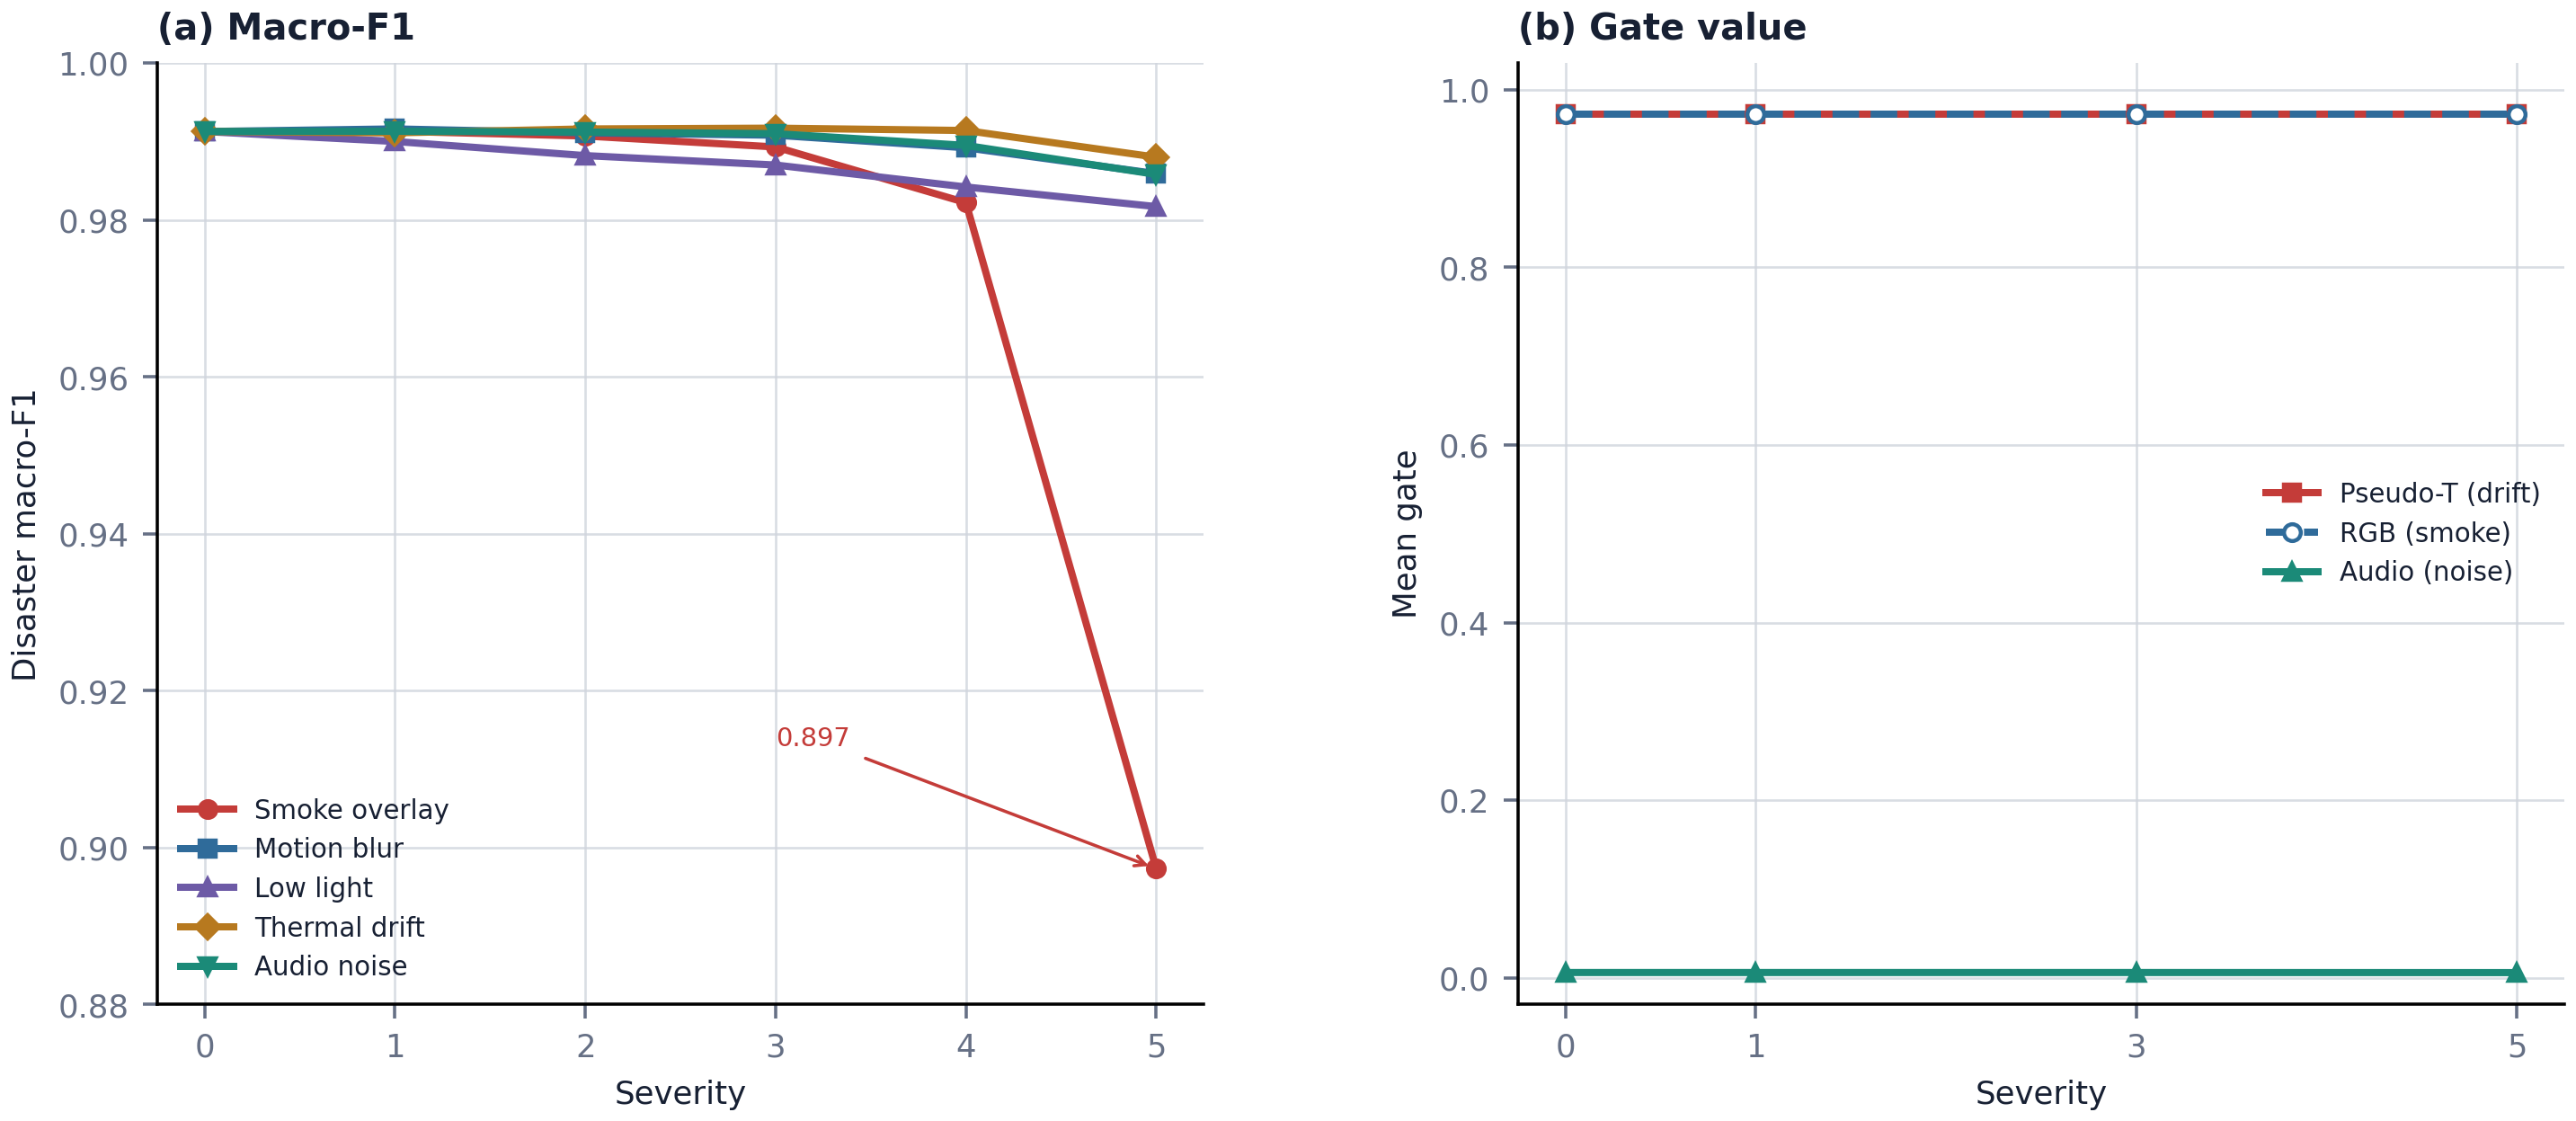
\includegraphics[width=0.8\textwidth]{fig_05_robustness.png}
\caption[Robustness under synthetic corruptions]{(A) AdapFuse-v1 disaster macro-F1 under five synthetic corruptions; severe smoke gives 0.897. (B) Mean modality gates: RGB and pseudo-thermal stay near 1 and audio near 0, so robustness comes from redundancy, not dynamic reweighting.}
\label{fig:robustness_stress}
\end{figure*}

Figure~\ref{fig:robustness_qualitative} grounds the aggregate sweep in one real FLAME test image processed under a clean input, a synthetic smoke overlay, and simulated RGB dropout. The predictions and gates are checkpoint outputs; the altered conditions themselves are synthetic.

\begin{figure*}[!t]
\centering
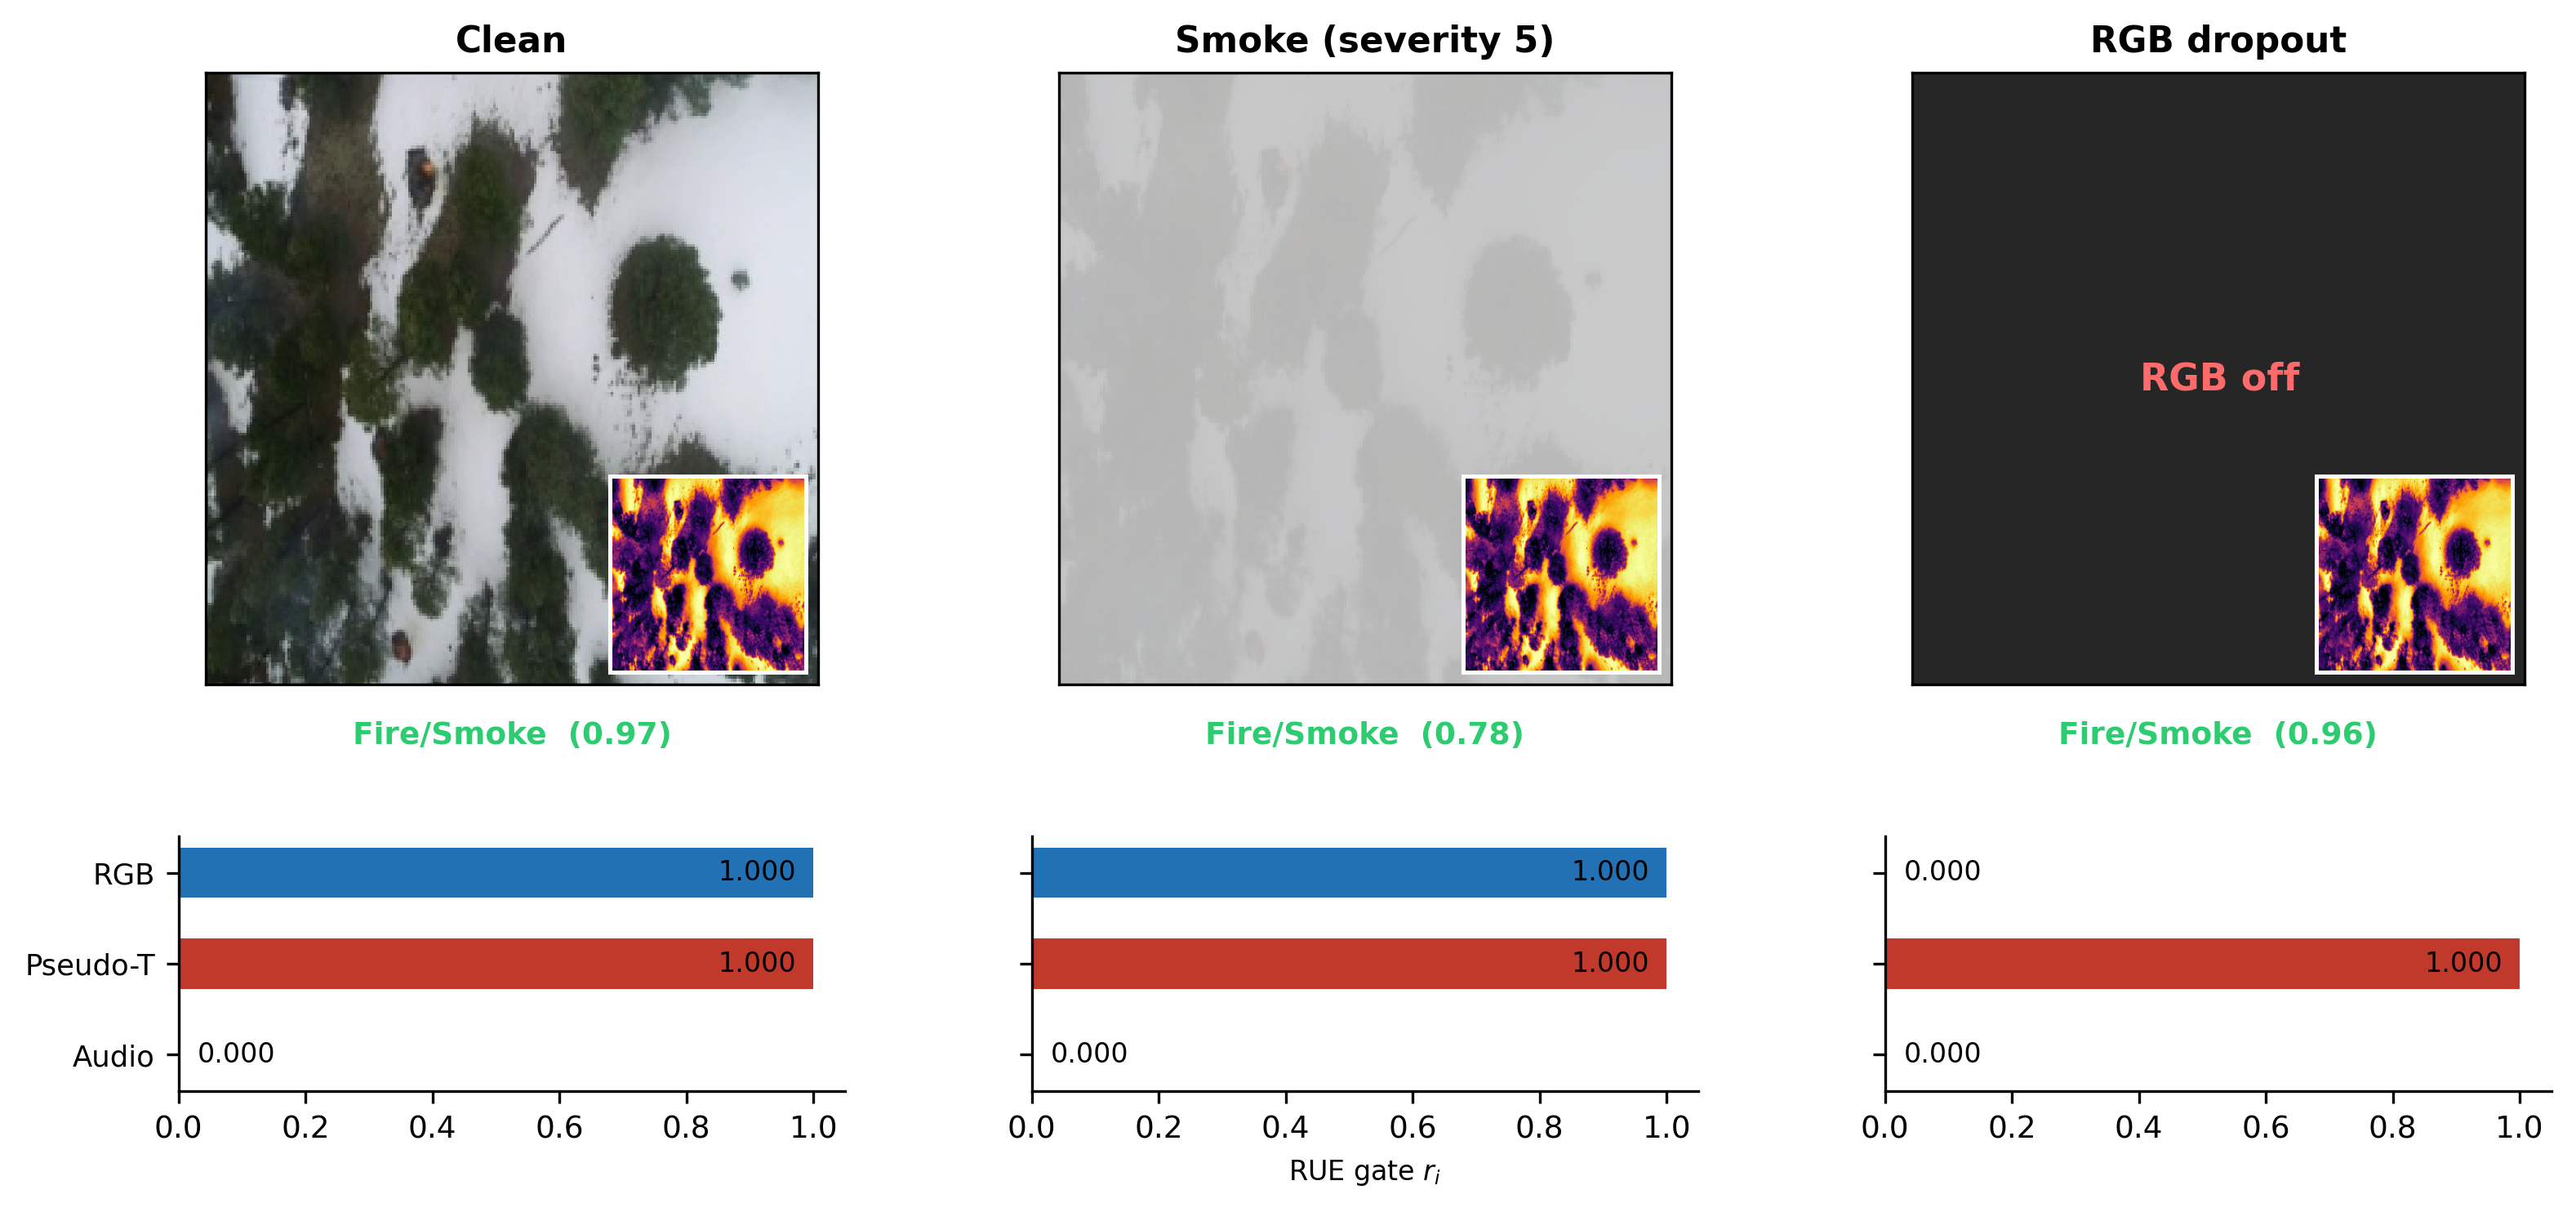
\includegraphics[width=0.8\textwidth]{fig_12_robustness_qualitative.png}
\caption[Predictions on one FLAME frame under corruption]{AdapFuse-v1 on one FLAME test frame: clean, synthetic smoke and RGB dropout. The prediction holds, but the RGB gate does not drop under smoke.}
\label{fig:robustness_qualitative}
\end{figure*}

\begin{enumerate}
    \item \textbf{Synthetic smoke overlay:} Disaster macro-F1 decreases from 0.9913 to 0.8973 at severity 5. Our mean RGB gate remains 0.9721 (the value obtained when every row with RGB has a gate of $\approx$1.0) rather than tracking the corruption; robustness is therefore more plausibly due to residual visual signal and redundancy with the RGB-derived pseudo-thermal input.
    \item \textbf{Pseudo-thermal drift:} Macro-F1 remains 0.9880 at severity 5, while the pseudo-thermal gate remains near 0.9721. This is a sensitivity result for transformed derived maps, not a radiometric sensor-drift experiment.
    \item \textbf{Motion blur:} Macro-F1 remains 0.9859 at severity 5, a 0.54\,pp decline from the clean 0.9913 baseline.
    \item \textbf{Low light:} Macro-F1 remains 0.9817 at severity 5, the second-largest decline after the smoke overlay.
    \item \textbf{Audio-noise transform:} Macro-F1 remains 0.9858 at severity 5. The audio gate is already near 0.006 before corruption and changes negligibly, consistent with this model largely ignoring the audio channel, so the sweep says little about robustness to acoustic noise.
\end{enumerate}

\subsection{Component-Wise Ablation Study of the AdapFuse-v1 Architecture}
\label{sec:component_ablations}

Five single-component variants were trained on the same row-level split and evaluated on the held-out test set ($n=10{,}951$). Table~\ref{tab:ablation_results} reports their descriptive differences from our base run. Because the repository does not contain repeated seeds or confidence intervals, these comparisons indicate associations rather than causal component effects. Two further facts limit them. First, the base run's logged learning rate cycles with a period of about eight epochs, whereas all five variants follow the configured single cosine decay (Table~\ref{tab:training}), so each comparison also changes the schedule. Second, removing the nuisance head changes no training signal, because its loss is already zero in the base run; ablation\_no\_nuisance is therefore effectively a re-run of the base model, and its 4.6$\times$ higher test loss with a $-0.02$\,pp change in combined F1 indicates the scale of run-to-run variation. Differences of a few tenths of a point, and loss ratios of 4--5$\times$, are within what this comparison can produce without any component effect.

\begin{table*}[!t]
\centering
\caption[Component ablations of AdapFuse-v1]{Component ablations of AdapFuse-v1 ($n=10{,}951$). Single runs; no repeated seeds or confidence intervals.}
\label{tab:ablation_results}
\resizebox{\textwidth}{!}{%
\begin{tabular}{@{}llcccccc@{}}
\toprule
\textbf{Model Variant} & \textbf{Component Removed} & \textbf{Test Loss} & \textbf{Dis.\ F1} & \textbf{Vic.\ F1} & \textbf{Comb.\ F1} & \textbf{$\Delta$ Comb.\ F1} & \textbf{Loss Multiple} \\
\midrule
\textbf{AdapFuse-v1 (Base Teacher)} & \textbf{None (Full Architecture)} & \textbf{0.0020} & \textbf{0.9913} & \textbf{0.9836} & \textbf{0.9874} & \textbf{n/a} & \textbf{1.0$\times$} \\
ablation\_no\_gru & Single-step GRU Refinement & 0.0102 & 0.9863 & 0.9765 & 0.9814 & \textbf{$-$0.60 pp} & 5.1$\times$ \\
ablation\_no\_attention & Cross-Modal Attention & 0.0076 & 0.9894 & 0.9785 & 0.9839 & \textbf{$-$0.35 pp} & 3.8$\times$ \\
ablation\_no\_quality\_tokens & Quality Token Heads & 0.0108 & 0.9881 & 0.9800 & 0.9840 & \textbf{$-$0.34 pp} & 5.4$\times$ \\
ablation\_no\_nuisance & NuisanceAwareHead & 0.0092 & 0.9923 & 0.9821 & 0.9872 & \textbf{$-$0.02 pp} & 4.6$\times$ \\
ablation\_no\_rue & RUE Reliability Gating & 0.0094 & 0.9938 & 0.9812 & 0.9875 & $+$0.01 pp$^*$ & 4.7$\times$ \\
\bottomrule
\end{tabular}%
}
\footnotesize{$^*$The no-RUE run is 0.01 percentage points higher in combined F1 but has 4.7$\times$ the base run's loss. Our stress-test logs do not contain a matched no-RUE corruption baseline, and the learned gates are nearly constant, so robustness cannot be attributed to dynamic reliability tracking.}
\end{table*}

\textbf{1. Single-Step GRU Refinement Changes the Learned Representation.}
Removing the GRU block (ablation\_no\_gru) corresponds to the largest difference in this suite: Combined F1 is 0.60 percentage points lower and victim-presence F1 is 0.71 points lower, while test loss is 5.1$\times$ higher. However, the implementation invokes the GRU with sequence length one (fused.unsqueeze(1)) and no carried-over hidden state, so each sample starts from a zero state and no information passes between frames. It therefore acts as a gated nonlinear refinement layer in these experiments; the result is not evidence of temporal smoothing, vibration invariance, or robustness across successive frames.

\textbf{2. The Attention Run Scores Slightly Above the Mean-Pooling Run.}
Replacing the 4-head attention block with token mean pooling (ablation\_no\_attention) corresponds to 0.35 percentage points lower combined F1 and 0.51 points lower victim-presence F1, with a 3.8$\times$ higher loss. The attention operates over three globally pooled modality tokens, not localized spatial patches. Moreover, the pseudo-thermal token is derived from the RGB image, so this experiment supports learned modality-level interaction but not independent RGB--thermal spatial correspondence.

\textbf{3. Learned Quality Features Are Associated with Lower Test Loss.}
Removing the dedicated 16-dimensional quality heads (ablation\_no\_quality\_tokens) corresponds to a 0.34-point lower combined F1 and a test loss of 0.0108 (5.4$\times$ the base run). This shows that the learned quality features are useful within the fitted architecture, but it does not establish calibrated uncertainty or detection of physical sensor degradation because no degradation targets are supplied during training.

\textbf{4. The Nuisance Variant Does Not Establish Nuisance Supervision.}
The no-nuisance run has a 4.6$\times$ higher loss but nearly unchanged combined F1. In our trainer, nuisance\_gt=None, so the base model's nuisance loss is also zero and the two runs differ only in the (unused) head, the random initialisation and the learning-rate schedule. The difference between these saved runs cannot therefore be interpreted as evidence that an auxiliary nuisance objective regularizes false-alarm features; it is better read as a measure of run-to-run noise, and repeated controlled runs with nuisance labels are required.

\subsection{Backbone Exploration and Architectural Augmentations}
\label{sec:backbone_variants}

\subsubsection{High-Capacity Visual Scaling: EfficientNet-B0 and MobileViT-XXS}
\begin{itemize}
    \item \textbf{EfficientNet-B0 (RGB):} Replacing MobileNetV3-Small with EfficientNet-B0~\cite{tan2019efficientnet} achieved the highest score among our runs: \textbf{99.24\% Combined F1} (Disaster F1: 99.23\%, Victim-presence F1: \textbf{99.24\%}, Victim-presence Accuracy: \textbf{99.47\%}). These are scene-level labels; no person size or location is evaluated.
    \item \textbf{MobileViT-XXS Hybrid Transformer:} Incorporating MobileViT-XXS~\cite{mehta2022mobilevit} for the RGB stream achieved \textbf{98.99\% Combined F1} and \textbf{99.16\% Victim-presence F1}. This supports the backbone as a competitive scene classifier on the present split, but does not by itself demonstrate survivor localization or edge-device operation.
    \item \textbf{EfficientNet-B0 (Pseudo-thermal):} Applying EfficientNet-B0 to the 1-channel RGB-derived maps achieved \textbf{98.80\% Combined F1} and \textbf{99.50\% Disaster Accuracy}. Because these inputs are algorithmically derived rather than radiometric LWIR measurements, the result does not test separation of physical heat sources from solar-heated clutter.
\end{itemize}
The RGB-only and pseudo-thermal-only versions of these backbones are reported in Tables~\ref{tab:unimodal_rgb} and~\ref{tab:unimodal_thermal}; with the backbone held fixed, the fused models score between 0.00 and 0.36 combined-F1 points higher.

\subsubsection{Acoustic Backbone Variants: GDBlock vs.\ CNN6-style Encoder}
Experiments comparing acoustic encoders (Table~\ref{tab:main_results}, Ranks 10, 16, 20) show that the multi-scale dilated \textbf{GDBlock} architecture reaches \textbf{98.63\% Combined F1} (0.0036 loss), while the \textbf{CNN6-style encoder} (``PANNS'' in the table) reaches \textbf{98.25\%} (0.0038 loss). The latter loaded no AudioSet convolution weights (Section~\ref{sec:backbone_selection}), so these runs do not test pretrained audio transfer, and because the ESC-50 clips are label-matched rather than synchronized to the visual scene, they are not an experiment with measured UAV rotor noise either. With the audio gate near zero, the 0.38-point gap between the two backbones mostly reflects how the rest of the network trains alongside each encoder, not the quality of disaster-relevant acoustic features, and neither result demonstrates audio--visual fusion. Trained alone (Table~\ref{tab:unimodal_audio}), both encoders reach the same degenerate solution, which suggests that their fused scores come mainly from the visual streams.

\subsubsection{Two-Sensor Subset Deployments}
\label{sec:two_sensor}
Evaluating two-channel subsets shows that \textbf{RGB + pseudo-thermal} reaches \textbf{98.50\% Combined F1} and \textbf{pseudo-thermal + audio} reaches \textbf{98.05\%}. These are metadata-channel ablations rather than hardware payload experiments. In particular, pseudo-thermal is computed from visible RGB, so the latter result does not establish a fallback for zero-visibility night or heavy-smoke operation: when the RGB frame is dark or occluded, the pseudo-thermal map derived from it is degraded in the same way. Likewise, the RGB + pseudo-thermal result combines two views of the same sensor and does not test fusion of independent sensors. A fallback evaluation requires independent LWIR hardware.

\subsubsection{Spatial Attention and Domain Prompt Tokens}
The \textbf{Spatial Attention} augmentation (adaptfuse\_v1\_spatial\_attn, 98.44\% F1) and \textbf{Domain Prompt Tokens} (adaptfuse\_v1\_domain\_prompts, 98.49\% F1) show that both modules can be added to the architecture with little change in row-level performance ($-0.30$ and $-0.25$ combined-F1 points relative to the 98.74\% base). Both are evaluated on the same row-level split as the base model, and the domain prompts are not supervised with condition labels; these results therefore show only that the modules do not degrade within-collection performance, not that they improve behaviour in specific flight regimes. Testing that claim would require held-out data from different altitudes, illumination, weather or sensor payloads.

\subsection{Error Analysis}
\label{sec:failure_gallery}

The near-ceiling aggregate metrics reported in Table~\ref{tab:main_results} can obscure specific failure modes. Figure~\ref{fig:failure_gallery} surfaces genuine misclassifications discovered by re-running trained checkpoints across the natural test set. AdapFuse-v1 errors are rare (8 found across 1{,}280 sampled test rows, consistent with its 99.44\% disaster accuracy) and concentrate on visually ambiguous clean-vs-collapse scenes, such as dense urban clutter mistaken for collapse debris. The audio-only baseline (A3, 38.2\% disaster F1) fails far more often (121 errors in a smaller sample) and defaults to Fire/Smoke, the expected output for rows without audio, which receive an all-zero input; this reflects missing and label-matched audio (Section~\ref{sec:unimodal_backbones}), not the acoustic quality of the clips.

\begin{figure*}[!t]
\centering
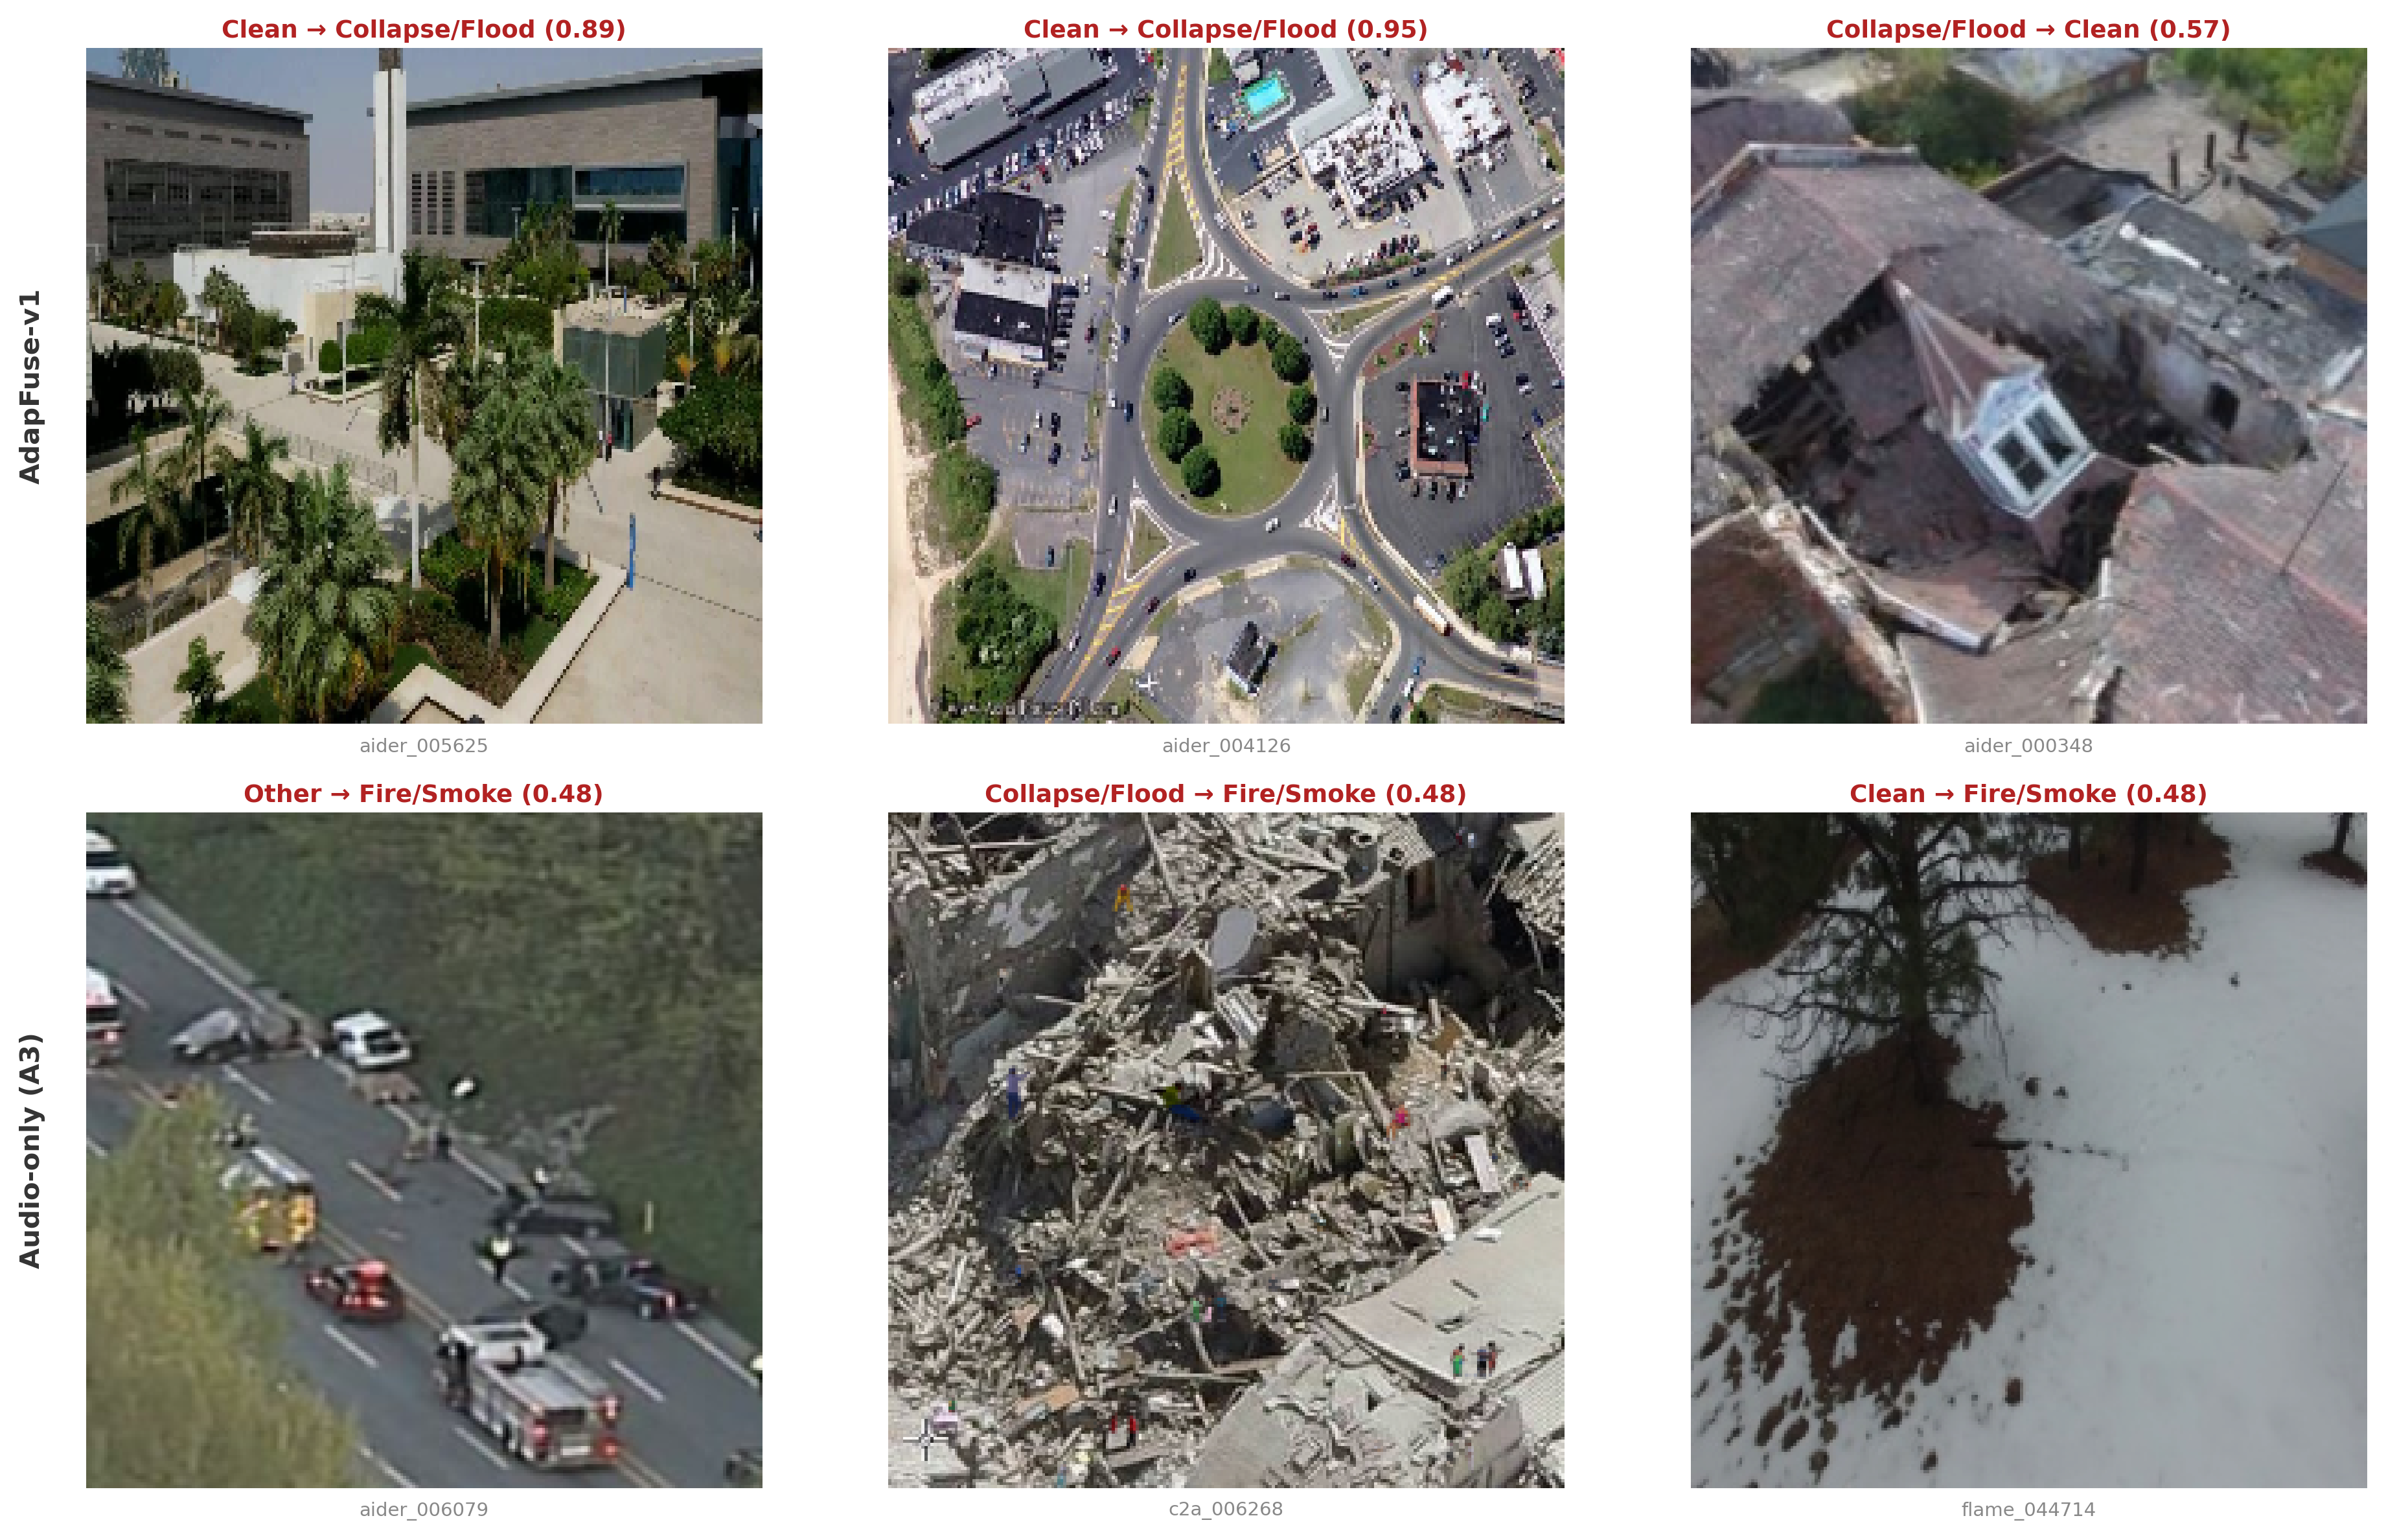
\includegraphics[width=0.8\textwidth]{fig_13_failure_gallery.png}
\caption[Real misclassifications]{Real misclassifications (true $\rightarrow$ predicted, confidence). Top: rare AdapFuse-v1 errors on ambiguous clean-vs-collapse scenes. Bottom: the audio-only baseline mostly predicts Fire/Smoke, its default output for rows without audio.}
\label{fig:failure_gallery}
\end{figure*}

\subsection{Summary of Key Findings}

\begin{enumerate}
    \item \textbf{Dense Object Detection Benchmark:} High-capacity YOLO26s (CLAHE) achieves $77.10\%\, \text{mAP}_{50}$ on D-Fire, while RT-DETRv2-R18 reaches $73.80\%$ and YOLO11n attains $72.25\%$.
    \item \textbf{HPG Is a Negative Result:} Hazard-YOLO26n reaches $70.53\%\, \text{mAP}_{50}$ in 8.65 hours versus $71.47\%$ in 4.45 hours for baseline YOLO26n under the same 40-epoch recipe, and its validation curve tracks the baseline's.
    \item \textbf{Multi-Task Prototype:} A revised recipe (curriculum warmup, stop-gradient isolation, distillation from AdapFuse-v1 and other changes) recovers scene classification to $99.26\%$ disaster accuracy and $98.57\%$ combined F1; the contribution of each change is not identified. The same saved evaluation reports detection $\text{mAP}_{50}=0.0$, and the logs show widespread non-finite losses in both joint runs, so successful joint localization is not established.
    \item \textbf{Fusion versus RGB-only:} On the row-level split, AdapFuse-v1 (98.74\% combined F1) does not exceed the RGB-only baseline (98.85\%), and the no-RUE variant (98.75\%) matches it; the fused inputs are RGB-derived or label-matched, so no fusion accuracy gain is shown.
    \item \textbf{Unimodal Backbones:} With three backbones per modality, the best RGB-only model (MobileViT-XXS, 98.99\%) matches the best-but-one fused model, and the best pseudo-thermal-only model (EfficientNet-B0, 98.60\%) improves on ResNet-18 by 1.17 points. With the backbone held fixed, fusion adds 0.00--0.36 points. The CNN6-style and GDBlock audio-only runs collapse to identical degenerate predictions.
    \item \textbf{Audio Label Leak:} On every row that has audio, the ESC-50 clip class identifies fire/smoke versus clean, and only these two classes have audio. The low audio-only macro-F1 reflects missing audio and absent classes, not uninformative audio, and any fused model can use the clip as a label shortcut.
    \item \textbf{Public Benchmarks:} Under the published AIDER 4:1:2 protocol, RGB-only EfficientNet-B0 reaches 94.00\% macro-F1 against 88.5\% for WATT-EffNet (trained from scratch), the best published result on that split. Under the official cross-camera FLAME protocol it reaches 83.72\% accuracy, above the original Xception (76.23\%) but below three later methods (85.12--88.05\%), with no-fire recall (75.8\%) as the main weakness; in-domain validation F1 is 99.9\% for every model. On our 70/20/10 D-Fire split (2{,}153 test images) our best detector (77.10\% mAP$_{50}$) is below the published YOLOv5l, YOLOv7x and YOLOv8 results (77.80--80.40\%, each reported on its own test set), mainly on fire AP. AdapFuse-v1 is below RGB-only EfficientNet-B0 on AIDER and FLAME. None of these results is state of the art.
    \item \textbf{Component Variants:} The base run outperforms the no-GRU, no-attention, and no-quality-feature runs by 0.60, 0.35, and 0.34 F1 points, respectively. These single-run differences are descriptive and of the same order as the run-to-run noise shown by the no-nuisance re-run; the variants also used a different learning-rate schedule from the base run, the GRU receives one step, reliability has no degradation targets, and the nuisance loss is zero.
    \item \textbf{Scene-Level Backbone Results:} EfficientNet-B0 reaches $99.24\%$ Combined F1 and MobileViT-XXS reaches $98.99\%$ on the row-level split. These results concern victim presence, not person localization.
    \item \textbf{Row-Level Error and Workstation Speed:} AdapFuse-v1 reports 0.73\% row-level scene-classification FPR, ECE 0.0337, and 14.32\,ms inference on an RTX 5090 workstation (32\,GB VRAM). Neither operational false-alarm reduction nor embedded-UAV speed has been validated.
    \item \textbf{Split and Source Effects:} Under a capture-group-aware split, combined macro-F1 falls from 98.74\% to 89.14\% (single seed). Victim presence is fully determined by source dataset in the grouped test set, so aggregate scores cannot separate person or hazard recognition from dataset recognition.
    \item \textbf{Reliability Gates:} In the row-level model the RGB and pseudo-thermal gates are saturated at $\approx$1.0 and the audio gate at $\approx$0.011 on rows with each input, unchanged under every synthetic corruption; the grouped retraining instead saturates the audio gate at 1.0 and switches pseudo-thermal off on 43.5\% of rows. The gates act as run-dependent on/off switches, and the RUE is not shown to track degradation.
\end{enumerate}


%=====================================================================
\section{Conclusion}
%=====================================================================

%*******************************************************************
% Chapter 9: Conclusion
%*******************************************************************

We presented UniAdapFuse, a reliability-aware multimodal fusion framework for UAV disaster perception, together with a physics-guided Hazard Prior Gate for smoke and fire detection. We evaluated twenty-six classification configurations on a 72{,}997-row corpus assembled from six public sources, seven detectors on the 21{,}527-image D-Fire benchmark, and a prototype joint graph. Throughout, our analysis distinguishes measured RGB from RGB-derived pseudo-thermal maps, label-matched audio from synchronized capture, and scene labels from bounding-box localization. It further separates within-collection from cross-sequence performance: retraining under a capture-group-aware split scores 9.60 percentage points lower in combined macro-F1, and decomposing those predictions by source shows that source identity and label are entangled in the assembled corpus.

The single most consequential finding is that the near-ceiling scores are inflated by row-level splitting and cannot be separated from source-label confounding. Retraining AdapFuse-v1 under a capture-group-aware split drops combined macro-F1 from 98.74\% to 89.14\% ($-9.60$ pp, single completed seed), with disaster classification losing 14.28 pp against the victim task's 4.93 pp. That retraining also disabled class balancing and used batch size 2, so the drop mixes leakage with recipe effects; a controlled rerun with the row-level recipe is needed to isolate the leakage component. The per-source decomposition (Section~\ref{sec:per_source}) shows that within-source accuracy is reasonable (0.82--0.998 for disaster), and that the low per-source macro-F1 values written by the evaluation script arise because classes absent from a source are scored as zero. It also shows the underlying problem: victim presence is fully determined by the source dataset in the grouped test set, SARD contains only clean scenes and FireNet only fire, so a model that recognises the dataset can score well without recognising people or hazards. The current experiments cannot rule this out, which qualifies every row-level number summarised below.

Within that qualification, the visual backbone variants are strong scene classifiers on the present split, with EfficientNet-B0 reaching 99.24\% combined F1 and MobileViT-XXS reaching 98.99\%; the victim metric is binary presence classification, and no person box, object size, or localization accuracy is measured. Fusion itself does not raise row-level F1: the RGB-only baseline (98.85\% combined F1) is 0.11 points above AdapFuse-v1 (98.74\%), and the no-RUE variant (98.75\%) matches it, so the reliability-aware design is supported here as an architecture that fuses heterogeneous inputs and runs with missing modalities, not as a source of accuracy gains. Retraining each single-modality baseline with three backbones confirms this: RGB-only MobileViT-XXS (98.99\%) equals the fused model with the same backbone, and with the backbone held fixed fusion adds at most 0.36 points. Trained through the same pipeline under published protocols, RGB-only EfficientNet-B0 exceeds the reported results on the AIDER 4:1:2 split (94.00\% macro-F1 against 88.5\%). On FLAME's cross-camera test it exceeds the original Xception baseline (83.72\% against 76.23\% accuracy) but stays 1.4--4.3 points below three later methods, because it rejects too few fire-free frames (75.8\% no-fire recall). On our 70/20/10 D-Fire split (2{,}153 test images) our best detector (77.10\% mAP$_{50}$) is 0.7--3.3 points below the published YOLOv8n and YOLOv7x results, which were reported on their own test sets. We therefore make no state-of-the-art claim. On FLAME, however, every model scores about 99.9\% on validation frames from the training drone and 17--37 points lower on the test drone, the same gap between within-capture and new-capture performance that the grouped split exposes. Among the compared fusion runs, AdapFuse-v1 attains the lowest loss, with Design E reporting loss 0.0020 and ECE 0.0337, although its 0.73\% false-positive rate is computed on the row-level scene-classification split and cannot be attributed to the nuisance head, whose loss is zero without nuisance labels. The component variants identify hypotheses for controlled follow-up rather than settled ablation results: relative to separate no-GRU, no-attention, and no-quality-feature runs, the base result is higher by 0.60, 0.35, and 0.34 combined-F1 points, but the repository has no repeated seeds or confidence intervals, the GRU receives sequence length one, and the nuisance comparison cannot demonstrate nuisance regularization because no nuisance targets are supplied.

The label-matched audio channel is not merely weak but leaky. The metadata reuse 2{,}000 ESC-50 clips across 39{,}003 assignments without synchronized UAV capture, and on every row with audio the clip's ESC-50 class identifies fire/smoke versus clean. The audio-only baseline's low 38.2\% disaster macro-F1 comes from missing audio on 47\% of test rows and from the absence of audio for the collapse and other-hazard classes, not from uninformative clips. The row-level model's audio gate settles near zero ($\approx$0.011 on rows with audio), whereas the grouped retraining opens it fully (1.0), consistent with that run using the shortcut. Data alignment, not acoustic backbone choice, is therefore the main limitation; because the intended AudioSet-pretrained encoder loaded no convolution weights, pretrained audio transfer was not tested either. The two-channel metadata variants remain competitive, with RGB plus pseudo-thermal reaching 98.50\% combined F1 and pseudo-thermal plus audio reaching 98.05\%, but because pseudo-thermal is derived from RGB these experiments do not validate zero-visibility or independent thermal-sensor operation.

On the joint and dense tasks, the revised joint recipe recovers classification in the prototype but not detection: UniAdapFuse v2 reaches 98.57\% combined F1 and 99.26\% disaster accuracy after the v1 classification collapse, yet its saved evaluation reports detection $\mathrm{mAP}_{50}=0.0$. The recovery combines stop-gradient isolation with distillation from AdapFuse-v1 and several other recipe changes, so it cannot be credited to isolation alone, and both joint runs show widespread non-finite losses, so dense joint detection remains unvalidated. Physical prior gating did not help on D-Fire: HPG YOLO26n reaches 70.53\% $\mathrm{mAP}_{50}$ in 8.65 hours against 71.47\% in 4.45 hours for baseline YOLO26n under the same 40-epoch recipe, with near-identical validation curves. Knowledge distillation, finally, yields only modest compression: AdapFuse-v2 halves the teacher's projection dimension with negligible accuracy loss ($<$0.2 percentage points combined F1), but because the dominant ResNet-18 and MobileNetV3-Small backbones are untouched, the measured total parameter reduction is 12.94M $\to$ 12.30M (4.9\%) rather than proportional to the projection-width halving. The teacher AdapFuse-v1 measures 14.32 ms per frame (69.9 FPS) on the evaluation workstation GPU, and dedicated benchmarking of AdapFuse-v2 on physical embedded edge hardware is identified as future work.

Reconciling these outcomes with the requirements set out in Chapter~3 makes several revisions explicit rather than leaving them as a silent gap between chapters, as is normal in an iterative research project. Chapter~3 called for at least 6{,}000 \textit{synchronised} (RGB, thermal, audio) sequences; our dataset instead pairs ESC-50 audio to visual samples by disaster label rather than by simultaneous capture, and every populated thermal path points to an RGB-derived pseudo-thermal map rather than a sensor measurement, so the near-constant audio gate ($r_{\text{audio}} \approx 0.006$) shows that the fitted model largely ignores this channel rather than proving calibrated reliability estimation. Chapter~3 also specified at least 95\% \textit{detection} accuracy for wildfire scenes and at least 90\% for USAR victim \textit{detection}; against these targets our system reports two distinct tasks, since scene-level \textit{classification} (99.4\% disaster accuracy, 98.36\% victim F1, Tables~\ref{tab:adaptfuse_extended} and~\ref{tab:main_results}) exceeds both thresholds on the row-level split while dense bounding-box \textit{detection} on D-Fire (Table~\ref{tab:dfire_results}) reaches 77.10\% mAP$_{50}$ for smoke/fire and no person/survivor bounding-box benchmark is reported (Section~\ref{sec:object_detection}, scope note). The thresholds were therefore met for row-level classification but not for dense object detection, and the two metrics should not be conflated. Relatedly, the architecture's Survivor RoI detection head (Section~\ref{sec:uniadaptfuse_arch}) is structurally implemented but never evaluated against ground-truth person bounding boxes in this work; only victim \textit{presence} classification is benchmarked, leaving person-level localisation evaluation, for example on SARD, to future work. Table~\ref{tab:req_trace} summarises the reconciliation.

\begin{table*}[!t]
\centering
\caption[Requirements against evidence]{Chapter~3 requirements against the evidence reported in Chapter~5.}
\label{tab:req_trace}
\resizebox{\textwidth}{!}{%
\begin{tabular}{@{}>{\raggedright\arraybackslash}p{3.0cm}>{\raggedright\arraybackslash}p{3.0cm}>{\raggedright\arraybackslash}p{4.4cm}>{\raggedright\arraybackslash}p{2.4cm}>{\raggedright\arraybackslash}p{4.6cm}@{}}
\toprule
\textbf{Requirement} & \textbf{Specification} & \textbf{Reported evidence} & \textbf{Status} & \textbf{Qualification} \\
\midrule
Wildfire detection & $\geq$95\% detection accuracy & 99.44\% disaster-classification accuracy (Table~\ref{tab:adaptfuse_extended}); 77.10\% smoke/fire mAP$_{50}$ on D-Fire (Table~\ref{tab:dfire_results}) & Met for classification only & Scene classification on the row-level split; grouped split gives 89.05\% accuracy; bounding-box detection is a different metric \\
\addlinespace
USAR victim detection & $\geq$90\% detection accuracy & 98.36\% victim-presence macro-F1 (Table~\ref{tab:adaptfuse_extended}) & Met for classification only & Presence label is determined by source dataset; no person bounding boxes evaluated \\
\addlinespace
False-positive rate & $\leq$8\% & 0.73\% row-level scene FPR (Table~\ref{tab:adaptfuse_extended}) & Met on row-level split & Not an operational field false-alarm rate; nuisance head unsupervised \\
\addlinespace
Graceful degradation & $\geq$85\% accuracy with any one modality missing & Two-sensor subsets 98.05--98.50\% combined F1 (Section~\ref{sec:two_sensor}) & Partially met & Pseudo-thermal derives from RGB, so losing RGB is not an independent-sensor test \\
\addlinespace
Latency & $\leq$500\,ms at $\leq$15\,W & 14.32\,ms on RTX 5090 workstation (Table~\ref{tab:latency_profile}) & Not validated & No embedded-hardware latency or power measured \\
\addlinespace
INT8 quantisation & All encoders & Not implemented & Not met & Future work \\
\addlinespace
Synchronised dataset & $\geq$6{,}000 synchronised tri-modal sequences & Pseudo-thermal from RGB; label-matched ESC-50 audio & Not met & No synchronised sensor data used \\
\bottomrule
\end{tabular}%
}
\end{table*}

Read against that boundary, this work makes four contributions to autonomous UAV aerial perception. The first is the UniAdapFuse prototype, a joint computation graph that combines multi-hazard scene classification, victim-presence classification, and a dense detection branch, in which a revised recipe (phased training, stop-gradient isolation and distillation) recovers classification to 98.57\% combined F1 while the recorded detection $\mathrm{mAP}_{50}$ remains 0.0; the contribution is thus an implemented prototype and a documented failure mode rather than a validated unified detector. The second is the Hazard Prior Gate, a physics-guided module that derives red-excess chromaticity, smoke achromaticity, and edge cues from the input and applies a bounded residual correction before the detector, together with the negative result that it neither raises accuracy (70.53\% against 71.47\% $\mathrm{mAP}_{50}$) nor shortens training (8.65 against 4.45 hours) for YOLO26n on D-Fire. The third is the audit of the reliability and nuisance mechanisms: the tri-modal architecture implements sigmoid modality gates and a nuisance branch, but in our models the gates saturate at 0 or 1, do not move across corruption severity, and differ between the row-level and grouped retraining (audio off in one, on in the other), and no degradation flags or nuisance labels are supplied by the trainer, so the audit establishes the implementation boundary and the experiments needed before dynamic reliability or nuisance suppression can be claimed. The fourth is reproducible comparative evidence, since the repository preserves results for multiple detector and classification configurations, component variants, provenance counts, and workstation latency, with AdapFuse-v2 containing 12.30M parameters against 12.94M for its teacher and the teacher measuring 14.32 ms on an RTX 5090 workstation (32\,GB VRAM), while embedded deployment remains future work.

Six directions follow directly from these limits. The highest priority is real UAV audio and multimodal synchronization: replacing label-matched ESC-50 audio with hardware-synchronized, UAV-embedded acoustic datasets such as DroneAudioset or DREGON is what would fully unlock acoustic complementary signals under rotor noise. Closely related is dynamic pre-backbone reliability estimation, upgrading the RUE to read pre-backbone physical quality signals such as optical flow variance, dark channel prior, or raw SNR, so that intra-modality degradation can be tracked dynamically under heavy smoke and glare. Third, out-of-distribution cross-dataset generalization should be quantified by evaluating the trained multi-modal and object detection models zero-shot on external aerial datasets such as HIT-UAV (aerial thermal imagery) and FLAME~2 (paired RGB and infrared wildfire frames), measuring domain transferability under varying altitudes and geographic biomes. Fourth, onboard flight testing and edge hardware profiling should deploy and profile the distilled AdapFuse-v2 and UniAdapFuse v2 models directly on embedded low-power accelerators aboard an autonomous UAV in real-world disaster simulation exercises. Fifth, a person/survivor bounding-box localization benchmark should evaluate the architecturally-implemented Survivor RoI head against ground-truth person boxes, for example on SARD, to complete the dense-detection evaluation alongside the existing smoke/fire results on D-Fire. Two further gaps follow from the component audit: the zero $\mathrm{mAP}_{50}$ of the joint UniAdapFuse v2 detector must be diagnosed (detection loss weighting, head learning rate, and the target and evaluation path are the first candidates) before joint perception can be claimed, and the GRU must be run on multi-frame sequences with carried-over hidden state before any temporal-modelling claim can be tested.

The sixth direction, source-decorrelated training and evaluation, is the one on which the credibility of every aggregate number depends. Capture-group-aware splitting has now been built and evaluated (Section~\ref{sec:grouped_split}), so near-duplicate leakage is measured rather than merely suspected, but three steps remain. The grouped run must first be repeated with the row-level recipe (class-balanced training, batch size 16), because our run changed both along with the split. The multi-seed interval must then be completed: of three launched seeds one finished cleanly, one selected its checkpoint during a window of degenerate validation, and one halted at epoch 12, so the grouped figure is currently a single-seed point estimate. More importantly, the per-source decomposition in Section~\ref{sec:per_source} shows that source identity and label are confounded in the assembled corpus (most starkly, victim presence is fully determined by source), so sources containing both values of each label, source-balanced class sampling, or leave-one-source-out evaluation are required before any aggregate score can be read as hazard or person discrimination rather than dataset recognition. The audio assignment must likewise be rebuilt so that the clip class no longer encodes the label, for example by pairing each visual row with a clip drawn independently of its label or, better, by using synchronized recordings.


%=====================================================================
\section*{Ethics Statement}

This work uses public benchmark datasets and does not report new data collection or direct interaction with human participants. Images and annotations are used only for research on disaster-scene perception. The victim-related output is a scene-level presence label, not identity recognition; no biometric identification is attempted. Because errors in an emergency setting could delay rescue or trigger unnecessary deployment, the models are research prototypes and must not be used as autonomous decision makers. Operational use requires source-grouped validation, representative field trials, human oversight, privacy review, and measurement on the intended UAV sensors and edge hardware.


% Can use something like this to put references on a page
% by themselves when using endfloat and the captionsoff option.
\ifCLASSOPTIONcaptionsoff
  \newpage
\fi

% references section
\bibliographystyle{IEEEtran}
\bibliography{references}

\end{document}
